\chapter{Search for new physics using boosted H bosons and missing energy}
\label{chap:analysis}

\section{Motivation \& Strategy}
\label{sec:mot}

If a more unifying theory than the SM exists it certainly has not been forthright in its manifestation. One possibility for the lack of discoveries of phenomena not explained within the SM is that there are indeed particles existing in nature which have not been observed, but they have such a large mass that the energy of the proton-proton collisions provided by the LHC is insufficient to directly create them. The outcome of many searches for new particles is thus the setting of limits placed on the cross section of their production mechanism. As these cross sections are dependent on the particle mass, the limits can be interpreted as setting lower bounds on the mass of any new physics - if the particle were any lighter than this limit it would have been produced copiously enough for its unambiguous detection (see for example \cite{CMS-SUS-16-033, CMS-SUS-15-002}). As these particles become more massive more momentum is imparted upon the particles involved in the final state; any SM particles resulting from the decay of higher mass states will be produced with large momentum (this is called high boost). As a particle becomes more boosted its decay products are emitted at smaller angles, eventually collimating enough to be reconstructed as a single jet. If new physics exists with masses accessible at the LHC, one could suspect that there exists non-zero coupling with the electroweak H, Z, or W bosons. Observation of events containing high-$p_{T}$ ($>$300 GeV) electroweak bosons are thus of considerable interest for finding new particles of large mass.

The Minimal Supersymmetric SM contains a $\mathbb{Z}_{2}$ symmetry in which all SM particles have charge -1 and all supersymmetric particles have charge +1, this is called R-parity \cite{susyprimer}. One direct consequence of R-parity is that the decay of a massive supersymmetric particle must include at least one supersymmetric particle in the final state. Necessarily this is the lightest such particle in the theory, denoted the lightest supersymmetric particle (LSP). If the LSP is electrically neutral it may escape detection, creating an imbalance in the net momentum of the event (similar to a neutrino). Therefore, events with a large momentum imbalance are also interesting as potential regions for SUSY.

With this as motivation, we designed an analysis searching for physics beyond the SM in events with boosted H or Z bosons and a large transverse momentum imbalance of the event. We reconstruct the H and Z bosons in the \bbbar decay mode, with 57\% and 15\% branching fractions, respectively. Although our analysis is sensitive to any new physics with this final state, we have adopted two benchmark models seen in Figure~\ref{fig:sms}. These are known as \textit{SMS} models and serve to simplify the SUSY parameter space into particle masses, cross sections, and branching fractions \cite{CMS-SUS-11-016}. In general, the diagrams begin with sparticle pair production which subsequently cascade decay to final states consisting of stable SM particles and a pair of stable supersymmetric particles which are the lightest in the theory. The blob in the figure indicates we are not interested in the particulars of the gluino production mechanism. Figures~\ref{fig:t5hh} and \ref{fig:t5zh} are known as the \textit{T5HH} and \textit{T5ZH} models respectively. The proton-proton interaction produces a pair of gluinos $\tilde{g}$ which decay to a neutralino $\tilde{\chi}_{2}^{0}$ along with the emission of SM quarks. This neutralino $\tilde{\chi}_{2}^{0}$ further decays into neutralino $\tilde{\chi}_{1}^{0}$ with the emission of a SM Higgs or Z boson.

\begin{figure}
\centering
\begin{subfigure}[b]{0.425\textwidth}
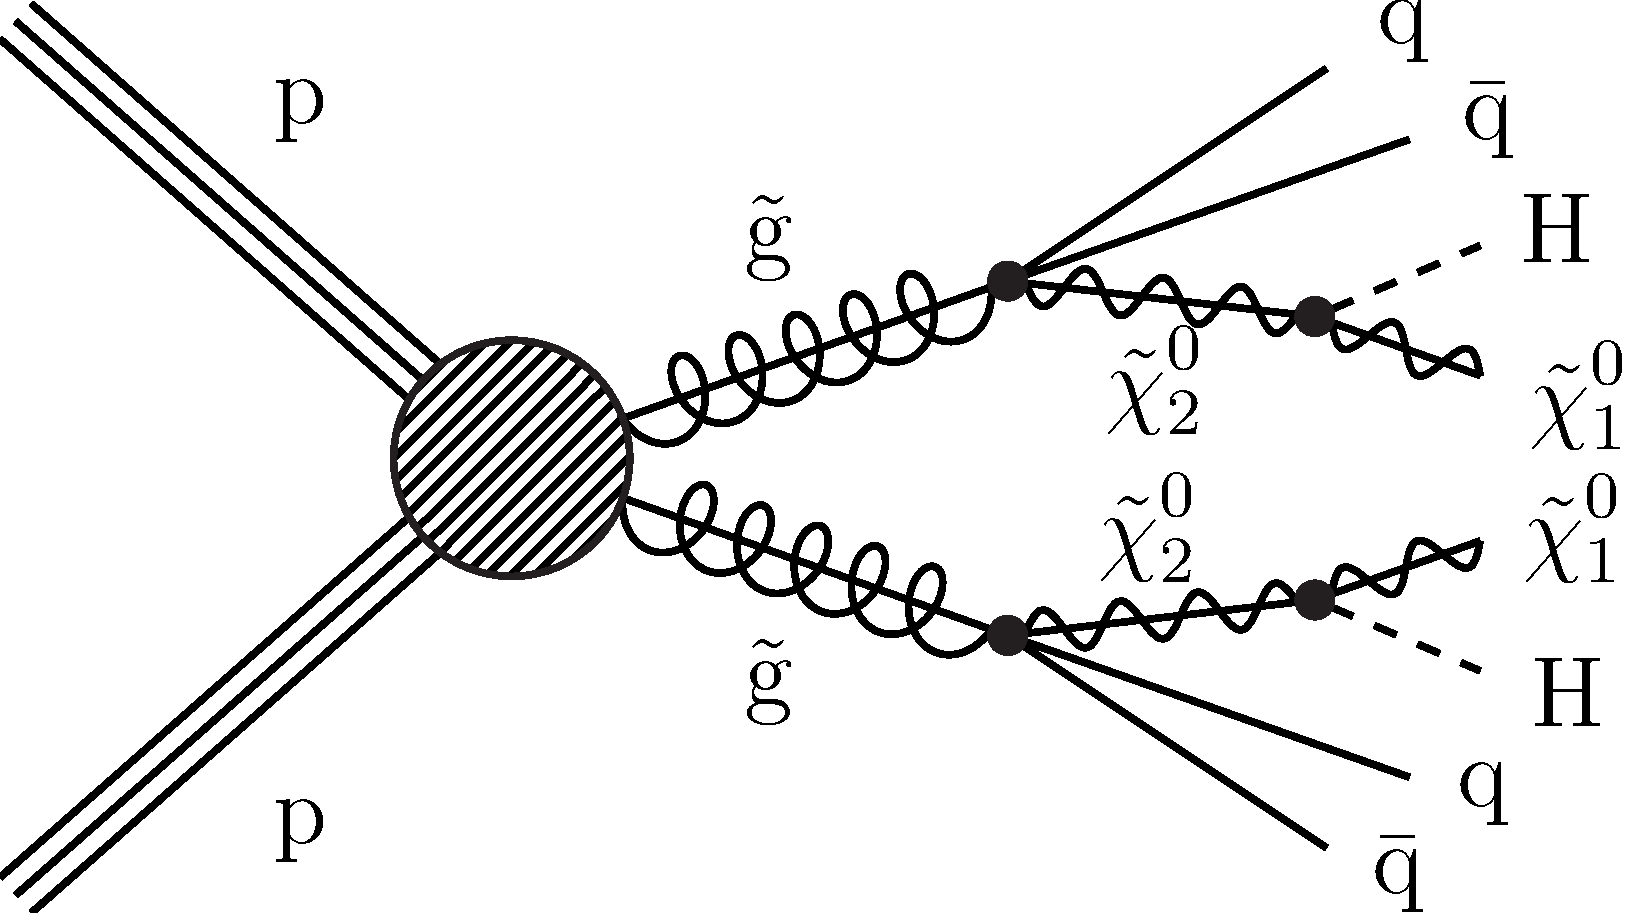
\includegraphics[width=0.95\textwidth]{figs/CMS-SUS-17-006_Figure_001.pdf}
\caption{The T5HH SMS model.}
\label{fig:t5hh}
\end{subfigure}
\begin{subfigure}[b]{0.425\textwidth}
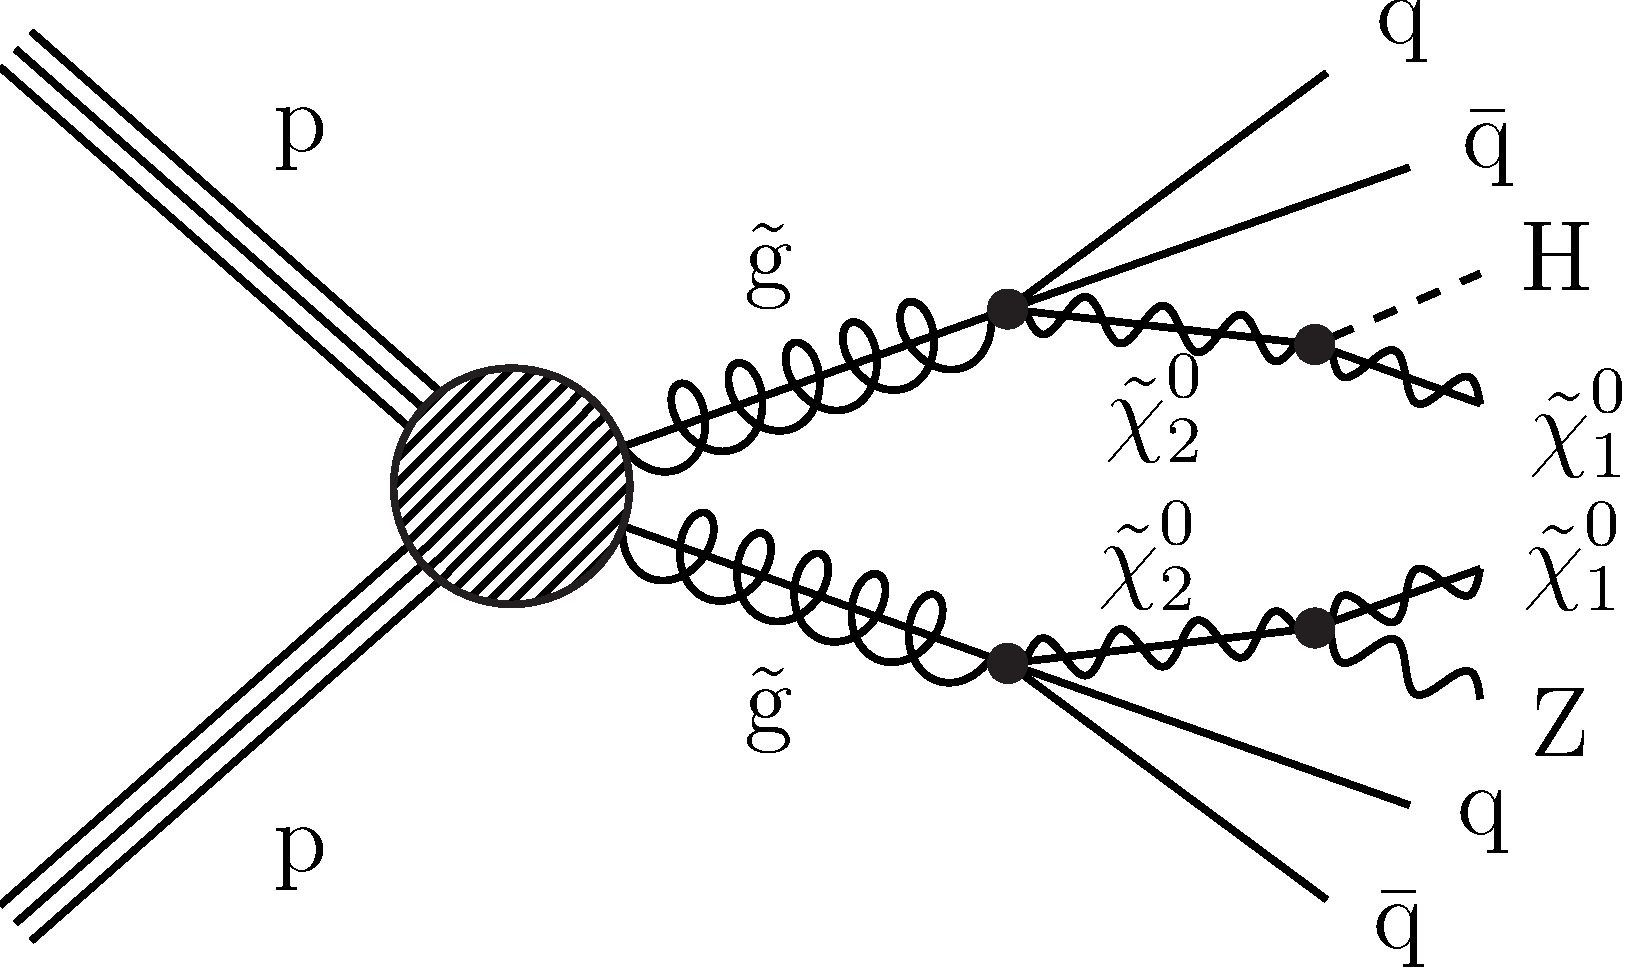
\includegraphics[width=0.95\textwidth]{figs/CMS-SUS-17-006_Figure-aux_001.pdf}
\caption{The T5ZH SMS model.}
\label{fig:t5zh}
\end{subfigure}
\caption{Diagrams of the benchmark models used for motivation of the targeted signal.}
\label{fig:sms}
\end{figure}

\section{Baseline Selection and Object Definition}
\label{sec:baseline}

The salient feature of our analysis is the presence of two high-\pt AK8 jets and large \ptmiss. Our most significant backgrounds are those that produce \ptmiss and can be divided into two categories depending on if it comes from a ``true'' or ``fake'' source. True \ptmiss arises from a neutrino or otherwise unobservable particle escaping our detector - a genuine imbalance in the detectable final-state momentum of the event. Fake \ptmiss arises from some sort of ``imperfection'' in our reconstruction process, for example the misidentification of a hadron. 

We approach our background as being constituted of three primary types. Two of them involve the production of neutrinos and the third is a result of jet resolution:

\begin{itemize}
\item $Z\rightarrow\nu\bar{\nu}$ in which the neutrinos from the Z decay results in true \ptmiss (`Z-invisible').
\item $W\rightarrow\ell\nu$ in which the lepton $\ell$ is not properly identified, resulting in the event not being vetoed, and the associated neutrino from the leptonic decay creating true \ptmiss (`lost-lepton'). The W boson can be produced through the decay of a top quark, either in single-top or \ttbar events; \ttbar events generate two W bosons, in which the other may decay into an AK8 jet. A W boson may additionally be produced directly in association with other jets.
\item Jet production via QCD in which the \pt of a jet is mis-measured, most commonly under-measured, creating a fake source of \ptmiss.
\end{itemize}

To mitigate these backgrounds, we establish a baseline selection choosing events with all-hadronic final states and missing transverse momentum (\ptmiss), as motivated by Figure~\ref{fig:sms}. The baseline selection is as follows:

\begin{itemize}
\item $\geq2$ AK8 jets, with $p_{T} > 300\,\mathrm{GeV}$ and $50 < \mathrm{mass} < 250\,\mathrm{GeV}$
\item $p_{T}^{\mathrm{miss}} > 300\,\mathrm{GeV}$;
\item no isolated electrons with $p_{T}>10\,\textrm{GeV}$:\newline
Isolation requires the $p_{T}$ sum of the particles within a cone of $\Delta R < 0.2$ to be less than 10\% of the electron $p_{T}$. (See \cite{miniiso} for details about ``mini-isolation''.)
\item no isolated muons with $p_{T}>10\,\textrm{GeV}$:\newline
The energy fraction for the isolation requirement is relaxed to 20\%.
\item no isolated tracks:\newline
To remove events with top or W production in which the W decays to a tau. As an isolated track is defined by looser criteria than that of an electron or muon, this cut also serves to increase the efficiency of the isolated electron and muon vetoes. Leptonic tracks must satisfy $p_{T}>5\,\textrm{GeV}$ and have 20\% isolation. Hadronic tracks must satisfy $p_{T}>10\,\textrm{GeV}$ and have 10\% isolation.
\item $\Delta\phi_{1, 2, 3, 4} > 0.5, 0.5, 0.3, 0.3$; $\Delta\phi_{i}\equiv \Delta\phi(\vec{p_{T}}^{\mathrm{miss}}, \mathrm{AK4\,jet}_{i})$\newline
This cut requires that the difference in $\phi$ between the \ptmiss vector and each of the four highest-p$_{T}$ jets is sufficiently large to remove events in which a jet has been under-measured giving rise to fake \ptmiss. If less than four AK4 jets are available the additional cuts are removed.
\end{itemize}

To tag jets from $H \rightarrow b\bar{b}$ a dedicated MVA algorithm has been developed by the CMS collaboration to discriminate these signal jets from those produced by QCD processes \cite{bbtagger}. The algorithm makes use of the kinematics expected by having secondary vertices arising from the b-quark decays. Discriminating variables include the number, mass, energy, and position of the secondary vertices in the jets. Additional variables include the distance of closest approach between the vertices and tracks (when projected backwards); tracks arising from displaced vertices are not expected to project back to the primary interaction point. The distribution of this discriminator for the two highest-p$_{T}$ AK8 jets are seen in the left and right panels of Figure~\ref{fig:ak8dists}; signal-like events peak towards larger values. To $b\bar{b}$ tag the AK8 jets we choose the loose working-point ($>$0.3) corresponding to an efficiency of approximately $70-80\%$ for $H \rightarrow b \bar{b}$ (see Figure~\ref{fig:effH}). The stacked histogram and solid lines shows the distribution after baseline selection for simulation and two representative signal points, respectively. Appendix~\ref{chap:bb} details the \bbbar-tagger in more depth.

Additionally, to tag H or Z bosons a requirement is made on the invariant mass of the jet. We use the mass of the so called ``pruned'' jet - a method involving removal of soft and wide-angle radiation inside the jet \cite{prunedmass}. The pruning is very powerful for discriminating QCD jets from those produced by heavy particle decay. Our tagging requires the jet mass to fall within a window [85, 135 GeV] to be consistent with that of the H boson. The distributions of the jet mass are seen in Figure~\ref{fig:ak8dists}. The same identification criteria are applied to tag an AK8 jet as either an H or Z boson (there is no distinction made).

\begin{figure}
\centering
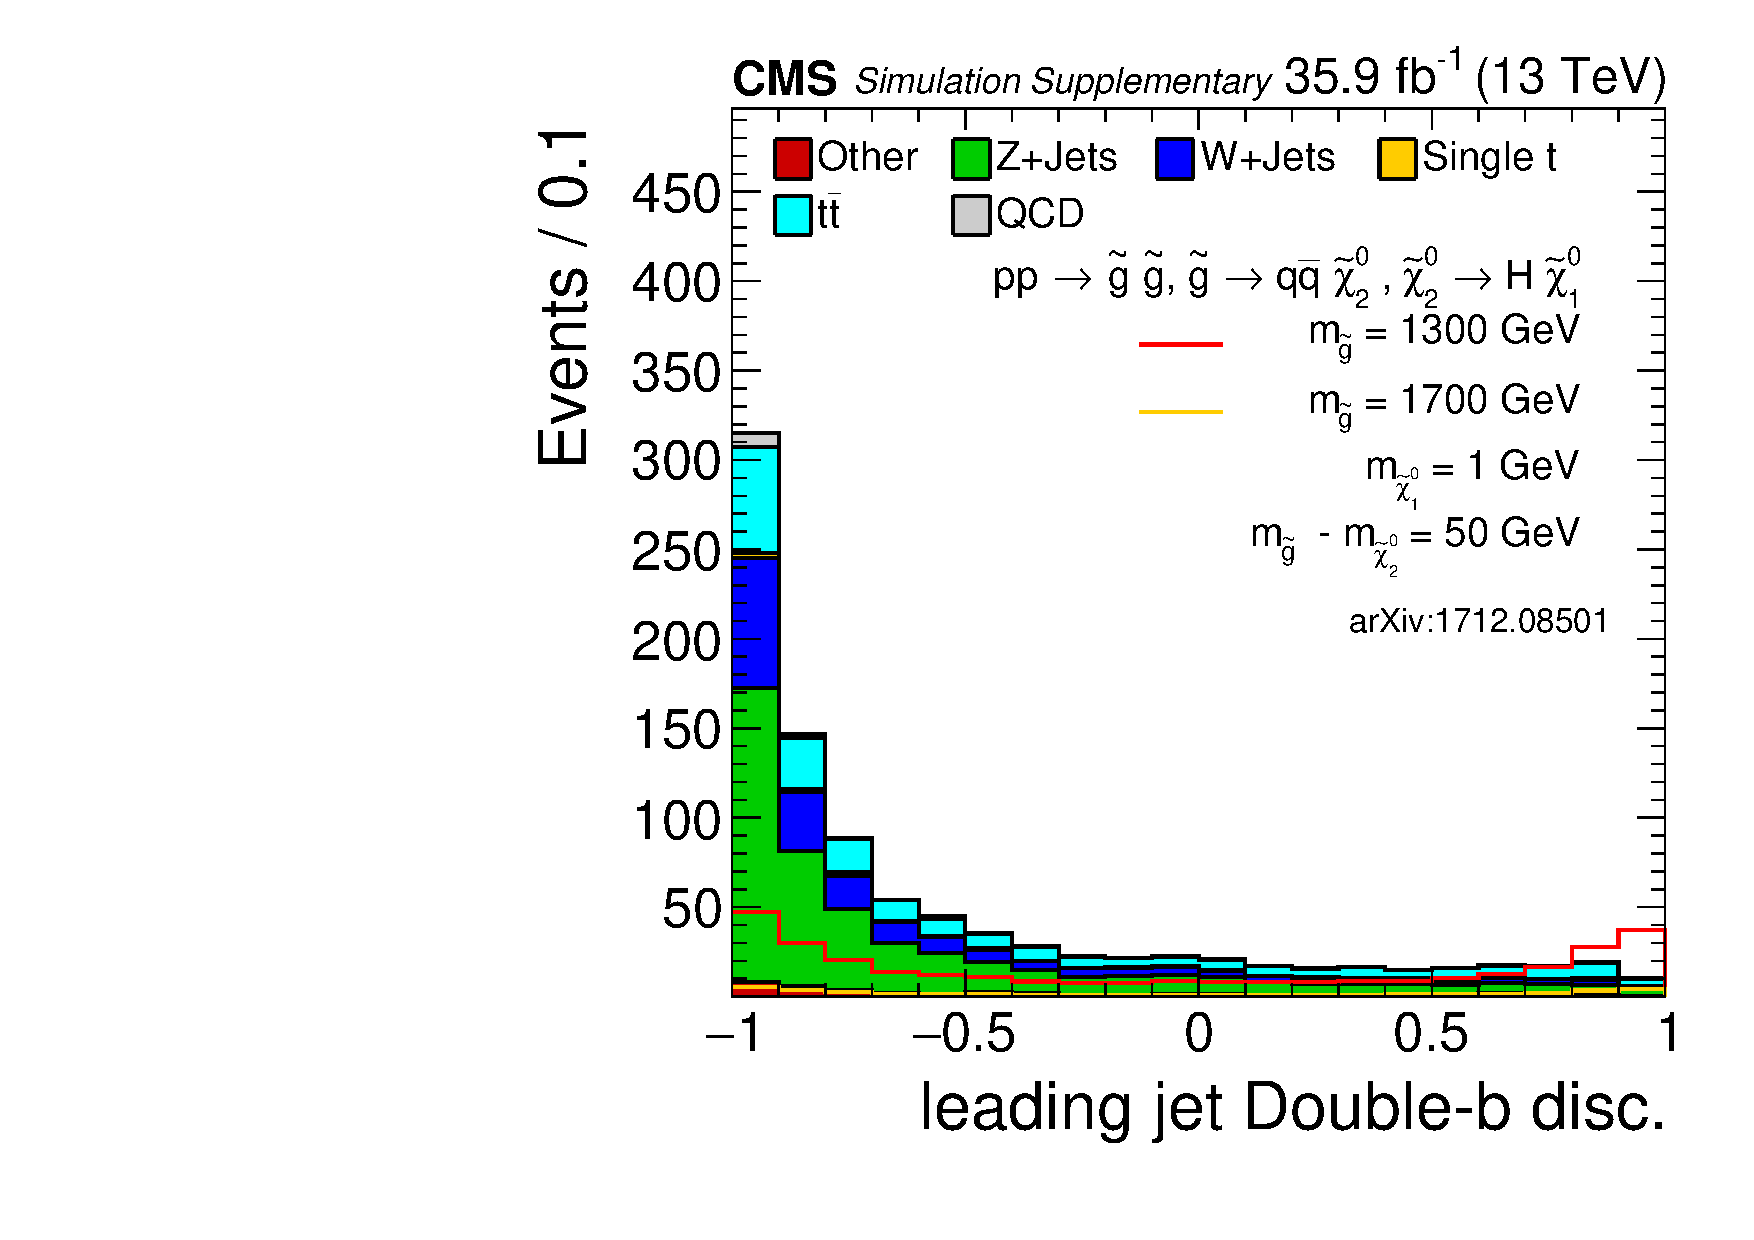
\includegraphics[width=0.425\linewidth]{figs/J1BB_LooseJetMass.pdf}
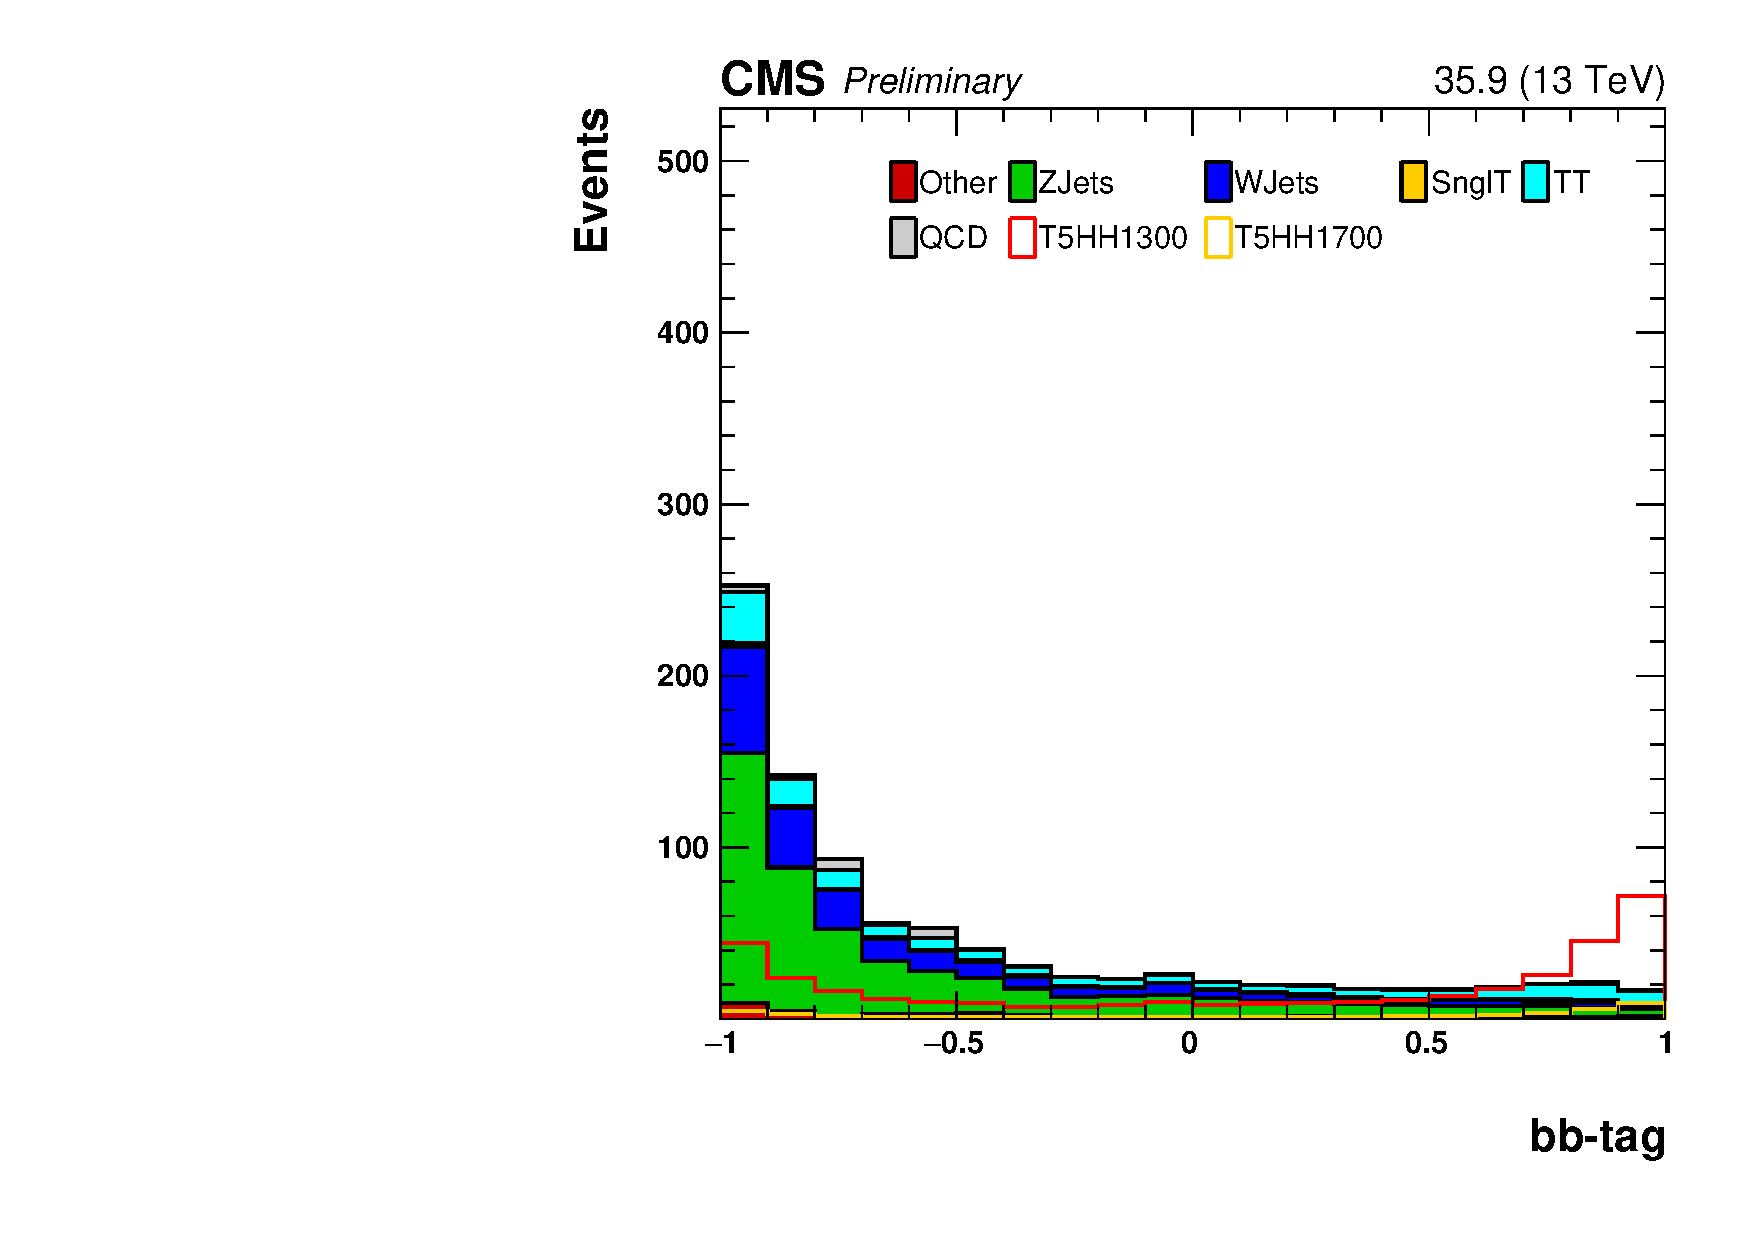
\includegraphics[width=0.425\linewidth]{figs/J2pt_BBtag_baseline.pdf}\\
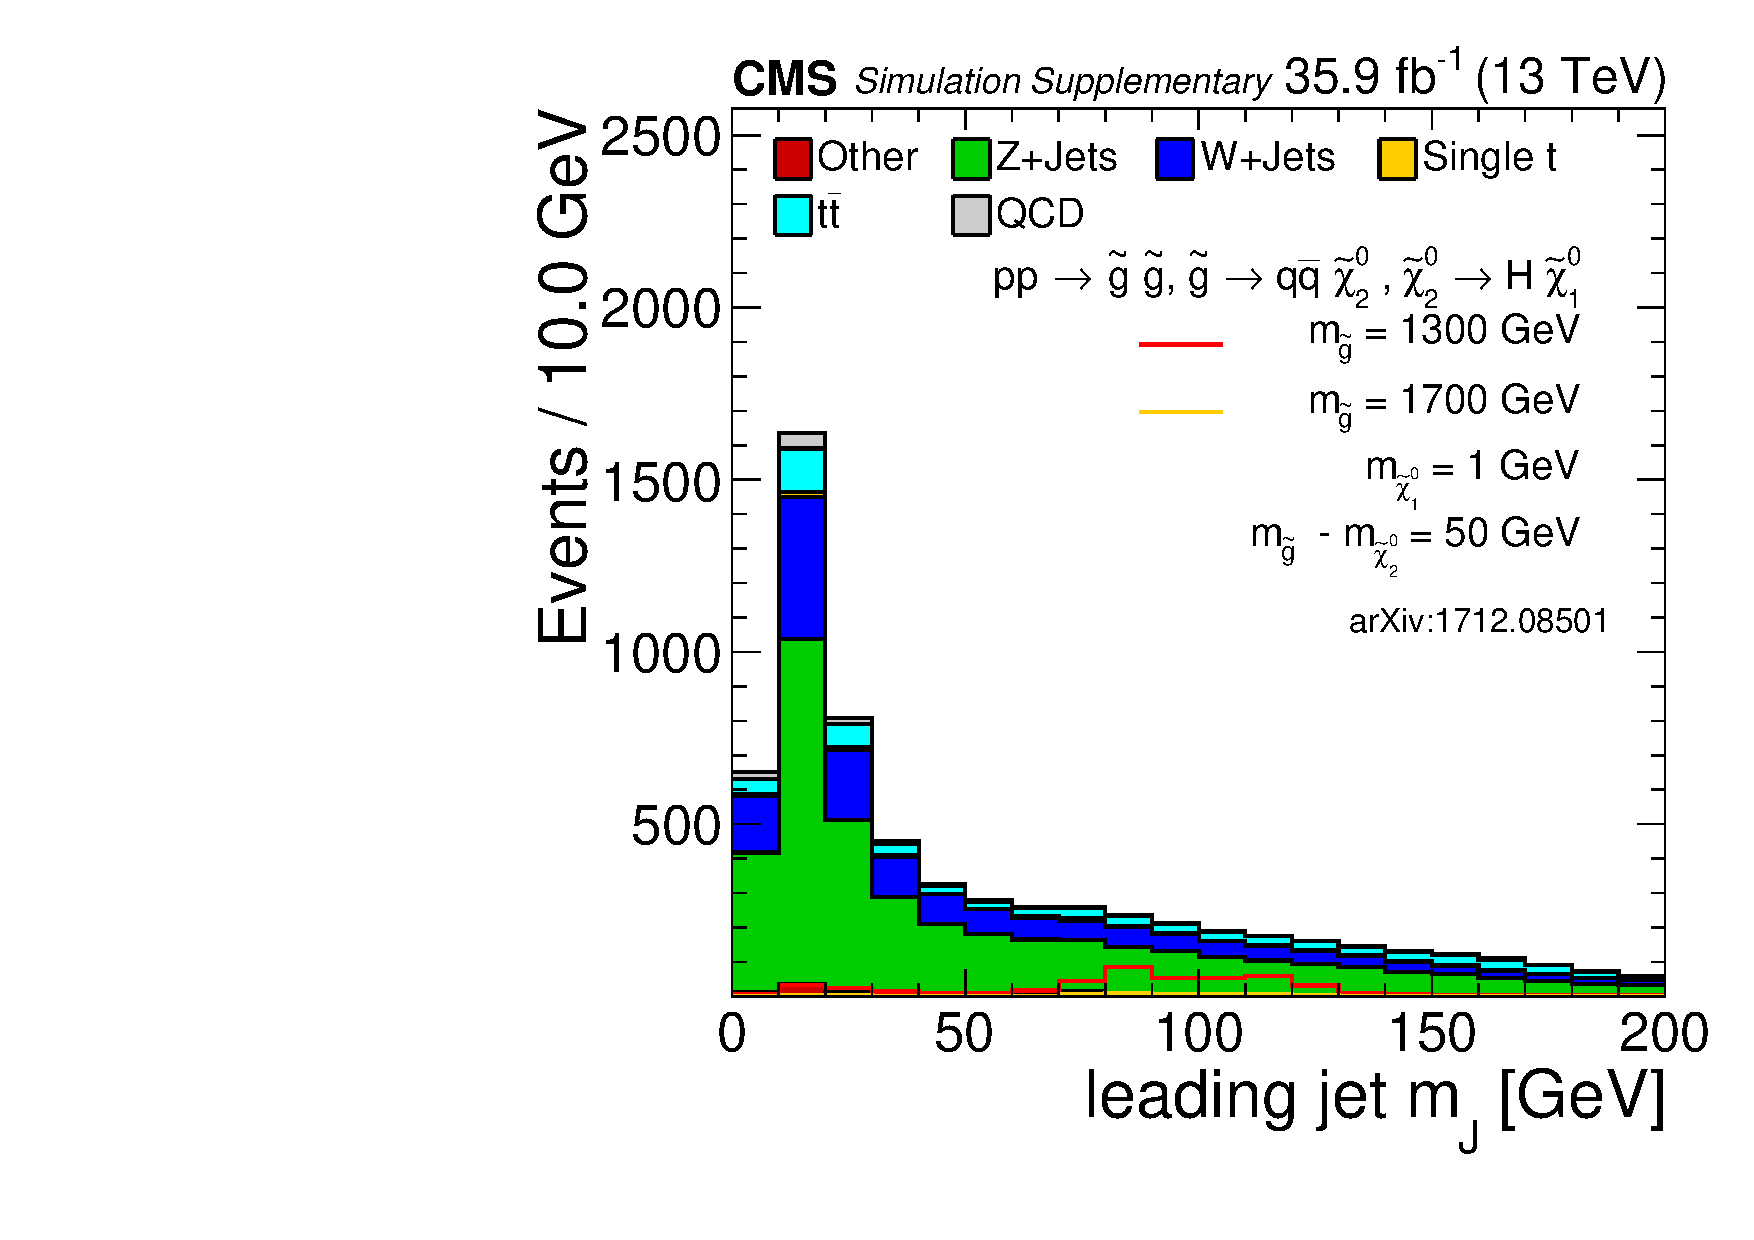
\includegraphics[width=0.425\linewidth]{figs/J1Mwide_JetPt.pdf}
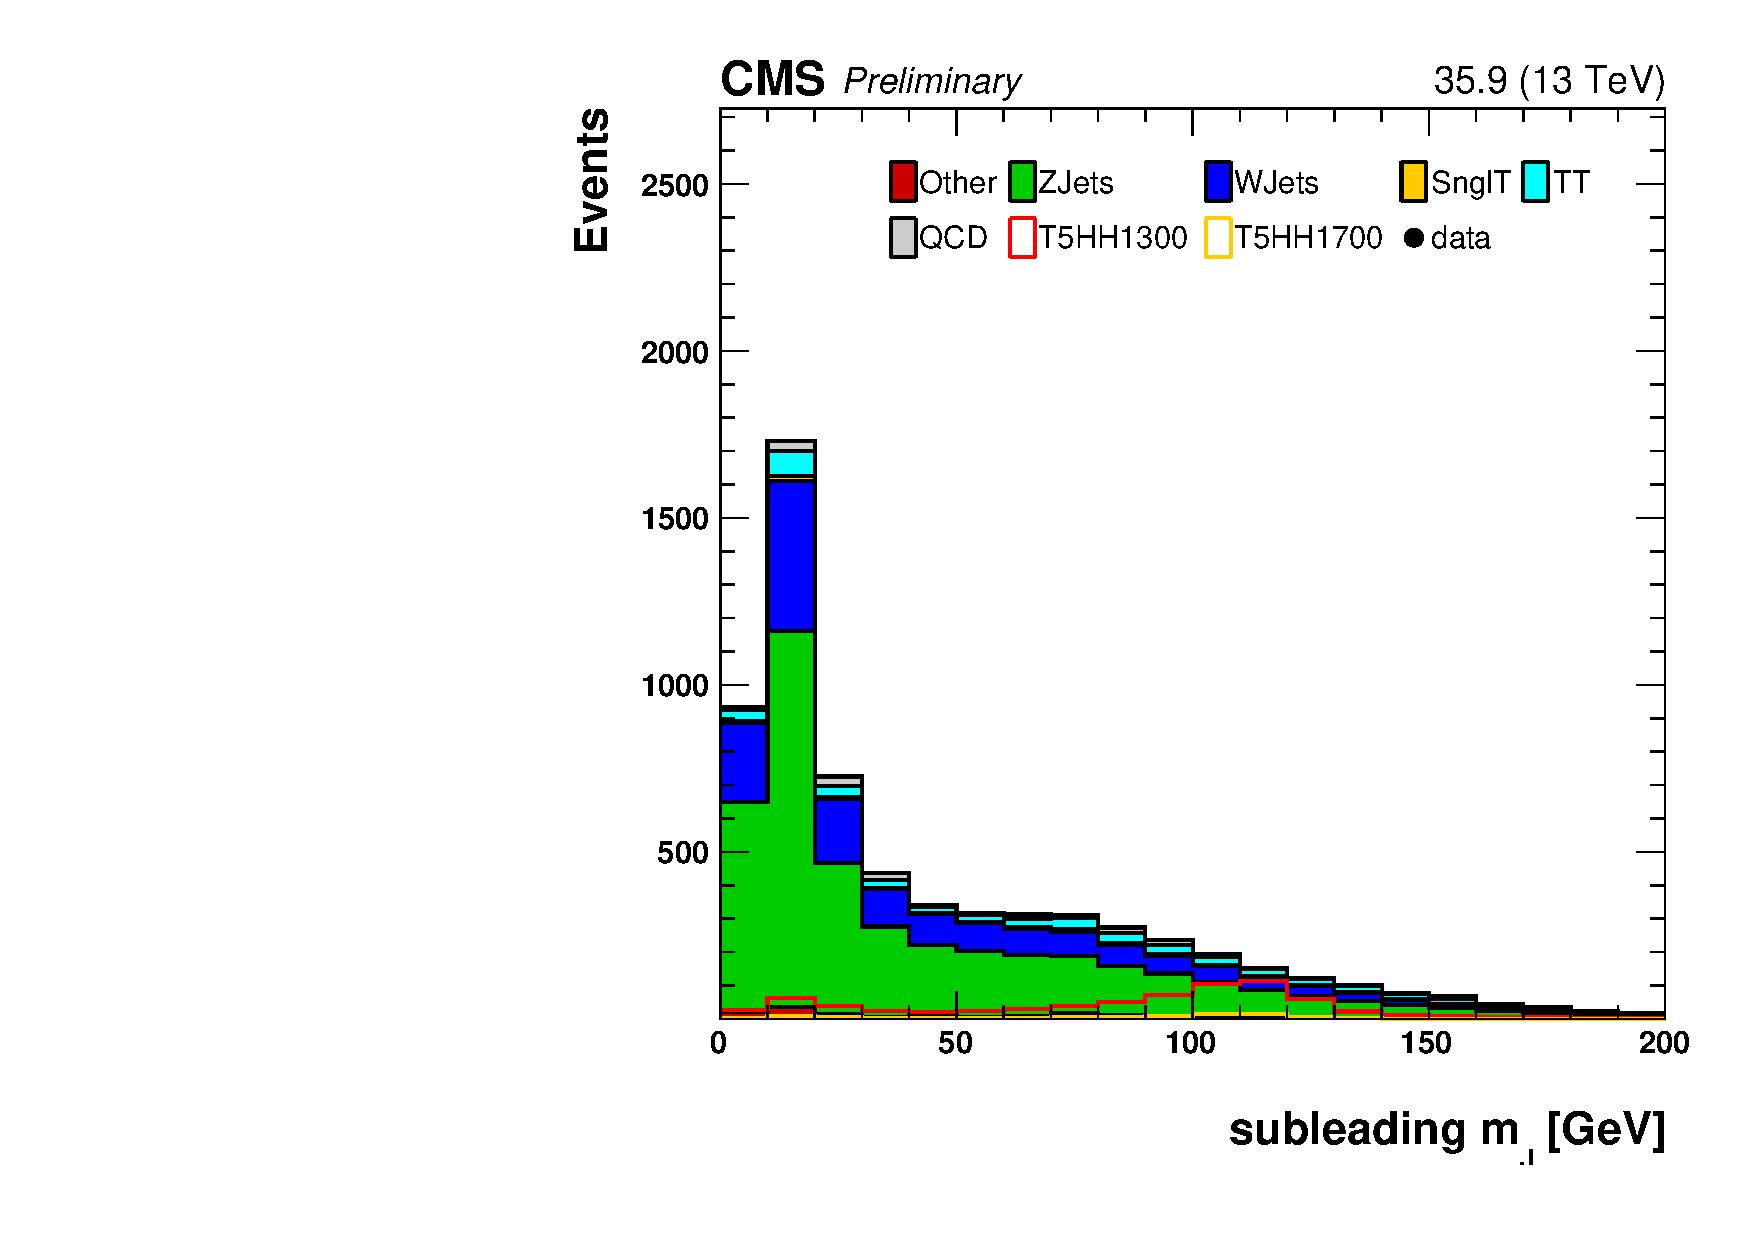
\includegraphics[width=0.425\linewidth]{figs/J2Mwide_JetPt.pdf}\\
\caption[Distributions of the bb-tagging discriminator and jet mass for AK8 jets.]
{Distributions of the bb-tagging discriminator (top row) and the jet mass (bottom row) for the highest (left column) and second highest (right column) $p_{T}$ AK8 jets. In the signal models, the H bosons are allowed to decay inclusively.}
\label{fig:ak8dists}
\end{figure}

\section{Dataset \& Trigger}

We use a total of 35.9 fb$^{-1}$ of data collected by the CMS experiment in 2016. Events are selected with the requirement of at least 100 GeV of \ptmiss calculated at high-level trigger (\texttt{HLT\_PFMET100\_PFMHT100\_IDTight}, HLT). To improve the trigger efficiency, the logical OR of similar triggers of thresholds 110, 120$\,$GeV are included.

The HLT is seeded at level-1 (L1) by the requirement of at least 100 GeV of missing transverse energy (\texttt{L1\_ETM100}). Missing transverse energy is calculated by the vectorial sums of the regional energy deposits in the calorimeters (and rotation by 180$^{\circ}$). This is additionally ORed with similar seeds of thresholds 90, 80, 70, 60, 50 GeV. Two additional ORed seeds require calorimeter jets with $p_{T}$ of at least 60 GeV (\texttt{L1\_ETM60\_Jet60\_dPhi\_Min0p4, L1\_DoubleJetC60\_ETM60}).

The trigger efficiency is defined as $\epsilon = N_{1}/N_{2}$, where $N_{2}$ is the total number of events passing baseline selection and $N_{1}$ is the total number of events selected by the trigger and passing baseline selection. In order to calculate this efficiency, we need to form an additional (hopefully independent) dataset by selecting events via a \textit{reference trigger}. Our reference trigger requires a single electron of $p_{T}>27\,\textrm{GeV}$, in addition to the baseline selection we require these events to contain at least three AK4 jets and exactly one reconstructed electron of $p_{T}>25\,\textrm{GeV}$. The signal region trigger is found to be greater than 98\% for events with \ptmiss$>$250 GeV and $H_{T}>300\,\textrm{GeV}$ \cite{CMS-SUS-16-033}. This is applied as a systematic error to the final results.

\section{Event Simulation}

Event simulation of the proton-proton collisions proceeds in several steps. MadGraph@NLO2.2.2 \cite{Alwall:2014hca} is a MC event generate used to simulate proton-proton events. Parton distribution functions, used to model the quark and gluon momenta distribution within the proton, are taken from NNPDF 3.0 \cite{Ball:2014uwa}. Parton showering, which models quark and gluon evolution into hadrons, or final/initial state radiation, is performed with Pythia \cite{pythiacite}. The final-state particles are traced through the detector using GEANT. For example, this includes the effect of the magnetic field, interactions with both the dead and sensitive detector material, and additional particle decay \cite{Agostinelli:2002hh}. This simulated data is processed in the same manner as that of the physical experiment.

\subsection{Standard Model Processes}
\label{sec:smp}

The SM samples which enter as the primary backgrounds are listed in Table~\ref{tab:MCsamples} (see Section~\ref{sec:smbkg} for a discussion of the background). All samples are generated with a pileup distribution with an average of 25 interactions per bunch crossing and a 25ns interval between bunches. For acceptable statistics over a wide range of parameter space, the  samples are often binned in $\mathrm{H_{T}} \equiv \sum_{AK4\,jets}p_{T}$. As our event selection requires at least two AK8 jets with $p_{T}>300\,\textrm{GeV}$ we roughly operate in the regime of $\mathrm{H_{T}}>600\,\textrm{GeV}$.

\begin{table}
\centering
\caption[SM samples used in the analysis.]{SM  samples used in the analysis. $\mathrm{H_{T}} \equiv \sum_{AK4\,jets}p_{T}$ is the total hadronic energy in the event. $\sigma$ is the cross section. $\int\mathcal{L} = N / \sigma$ is an alternative way to express the number of generated events.}
\label{tab:MCsamples}
\begin{tabular}{cclll}
\hline \hline
process & final state & $H_{T}$ (GeV) & $\sigma$ (pb) & $\int\mathcal{L}$ (fb$^{-1}$)\\
\hline
\ttbar & $t\rightarrow\ell\nu, \bar{t}\rightarrow2q$ & inclusive & 182.72 & 283.90\\
\ttbar & $\bar{t}\rightarrow\ell\nu, t\rightarrow2q$ & inclusive & 182.72 & 326.48\\
\ttbar & $2\ell$    & inclusive & 88.34 & 346.25\\
\ttbar & inclusive & [600, 800] & 2.734 & 5231.81\\
\ttbar & inclusive & [800, 1200] & 1.121 & 9416.61\\
\ttbar & inclusive & [1200, 2500]  & 0.198 & 14819.34\\
\ttbar & inclusive & [2500, $\infty$] & 0.002 & 221088.29\\
QCD & inclusive & [200, 300] & 1735000 & 0.03\\
QCD & inclusive & [300, 500] & 366800 & 0.16\\
QCD & inclusive & [500, 700] & 29370 & 1.95\\
QCD & inclusive & [700, 1000] & 6524 & 6.68\\
QCD & inclusive & [1000, 1500] & 1064 & 12.62\\
QCD & inclusive & [1500, 2000] & 121.5 & 32.63\\
QCD & inclusive & [2000, $\infty$] & 25.42 & 239.30\\
Z+jets & $\nu\bar{\nu}$ & [100, 200] & 344.8 & 54.13\\
Z+jets & $\nu\bar{\nu}$ & [200, 400] & 95.53 & 208.46\\
Z+jets & $\nu\bar{\nu}$ & [400, 600] & 13.20 & 77.30\\
Z+jets & $\nu\bar{\nu}$ & [600, 800] & 3.148 & 1795.26\\
Z+jets & $\nu\bar{\nu}$ & [800, 1200] & 1.451 & 1486.09\\
Z+jets & $\nu\bar{\nu}$ & [1200, 2500] & 0.355 & 1029.81\\
Z+jets & $\nu\bar{\nu}$ & [2500, $\infty$] & 0.0085 & 47498.87\\
W+jets & $\ell\nu$ & [100, 200] & 1627.45 & 18.16\\
W+jets & $\ell{\nu}$ & [200, 400] & 435.24 & 45.88\\
W+jets & $\ell{\nu}$ & [400, 600] & 59.18 & 123.64\\
W+jets & $\ell{\nu}$ & [600, 800] & 14.58 & 221.32\\
W+jets & $\ell{\nu}$ & [800, 1200] & 6.66 & 1123.13\\
W+jets & $\ell{\nu}$ & [1200, 2500] & 1.608 & 153.44\\
W+jets & $\ell{\nu}$ & [2500, $\infty$] & 0.039 & 6497.28\\
\hline \hline
\end{tabular}
\end{table}

\subsection{Signal Models}
\label{sec:signal-models}

For commissioning of the analysis technique (as well as the limit-setting procedure, see Section~\ref{sec:results}) Monte Carlo samples with our final-state signal topology were generated, based on the processes in Figure~\ref{fig:sms}. The signal sample follows the same processing chain as the SM samples. The mass splitting between the gluino $\tilde{g}$ and neutralino $\tilde{\chi}_{2}^{0}$ is fixed to 50 GeV, resulting in low $p_{T}$ SM quarks produced in the gluino $\tilde{g}$ decays. The mass of the neutralino $\chi^{0}_{1}$ (LSP) is fixed to 1 GeV. We have samples with a range of gluino $\tilde{g}$ masses from 750 to 2200 GeV. The $p_{T}$ distribution for the generated H bosons in these samples is seen in Figure~\ref{fig:GenHiggsBoost} for a number of gluino $\tilde{g}$ masses. Additionally the angular separation $\Delta R \equiv \sqrt{\Delta\phi^{2}+\Delta\eta^{2}}$ between the $b\bar{b}$ pair is shown. As the $p_{T}$ of a parent boson increases the $b\bar{b}$ pair from its decay tend to align, allowing complete reconstruction with a single AK8 jet. The distributions in Figure~\ref{fig:GenHiggsBoost} motivate our use of two such high-\pt AK8 jets.

\begin{figure}
\centering
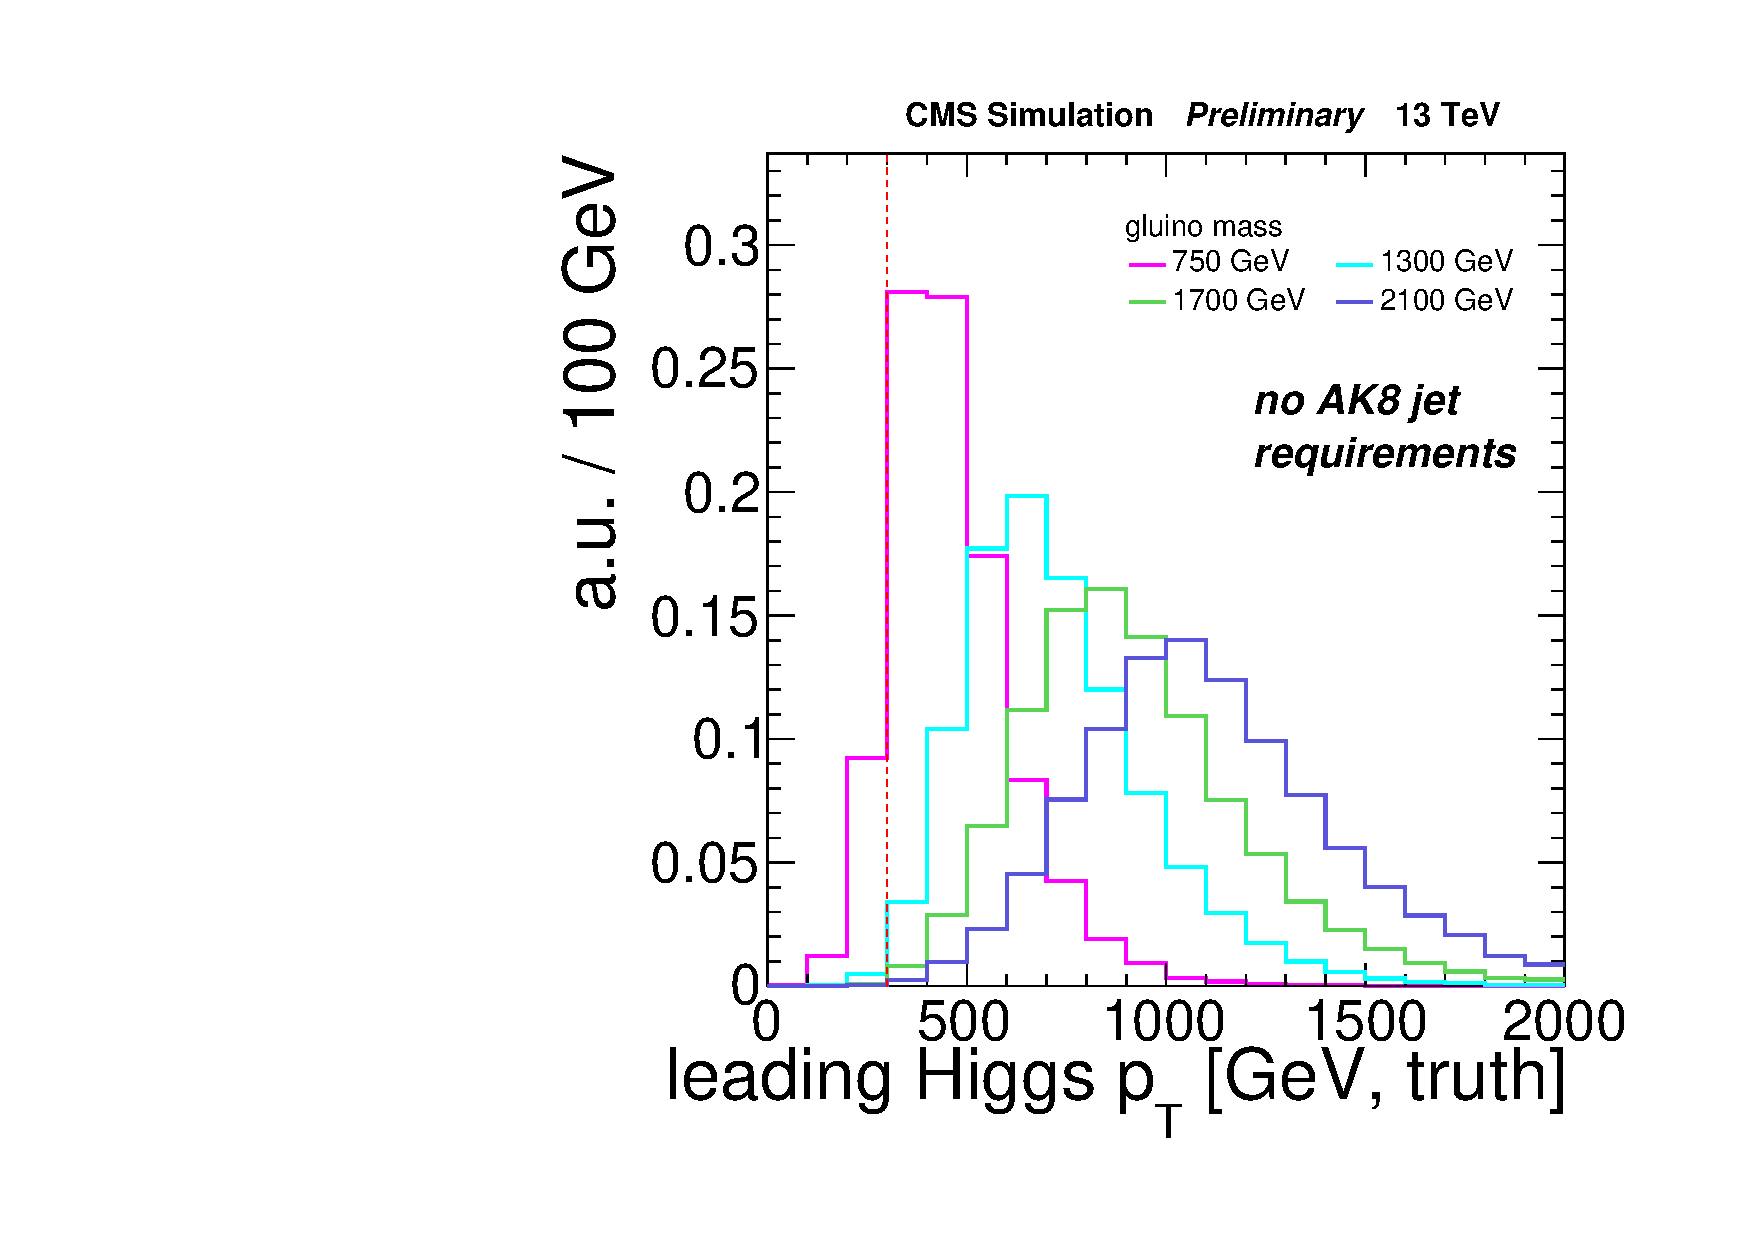
\includegraphics[width=0.425\linewidth]{figs/leadHiggsPt.pdf}
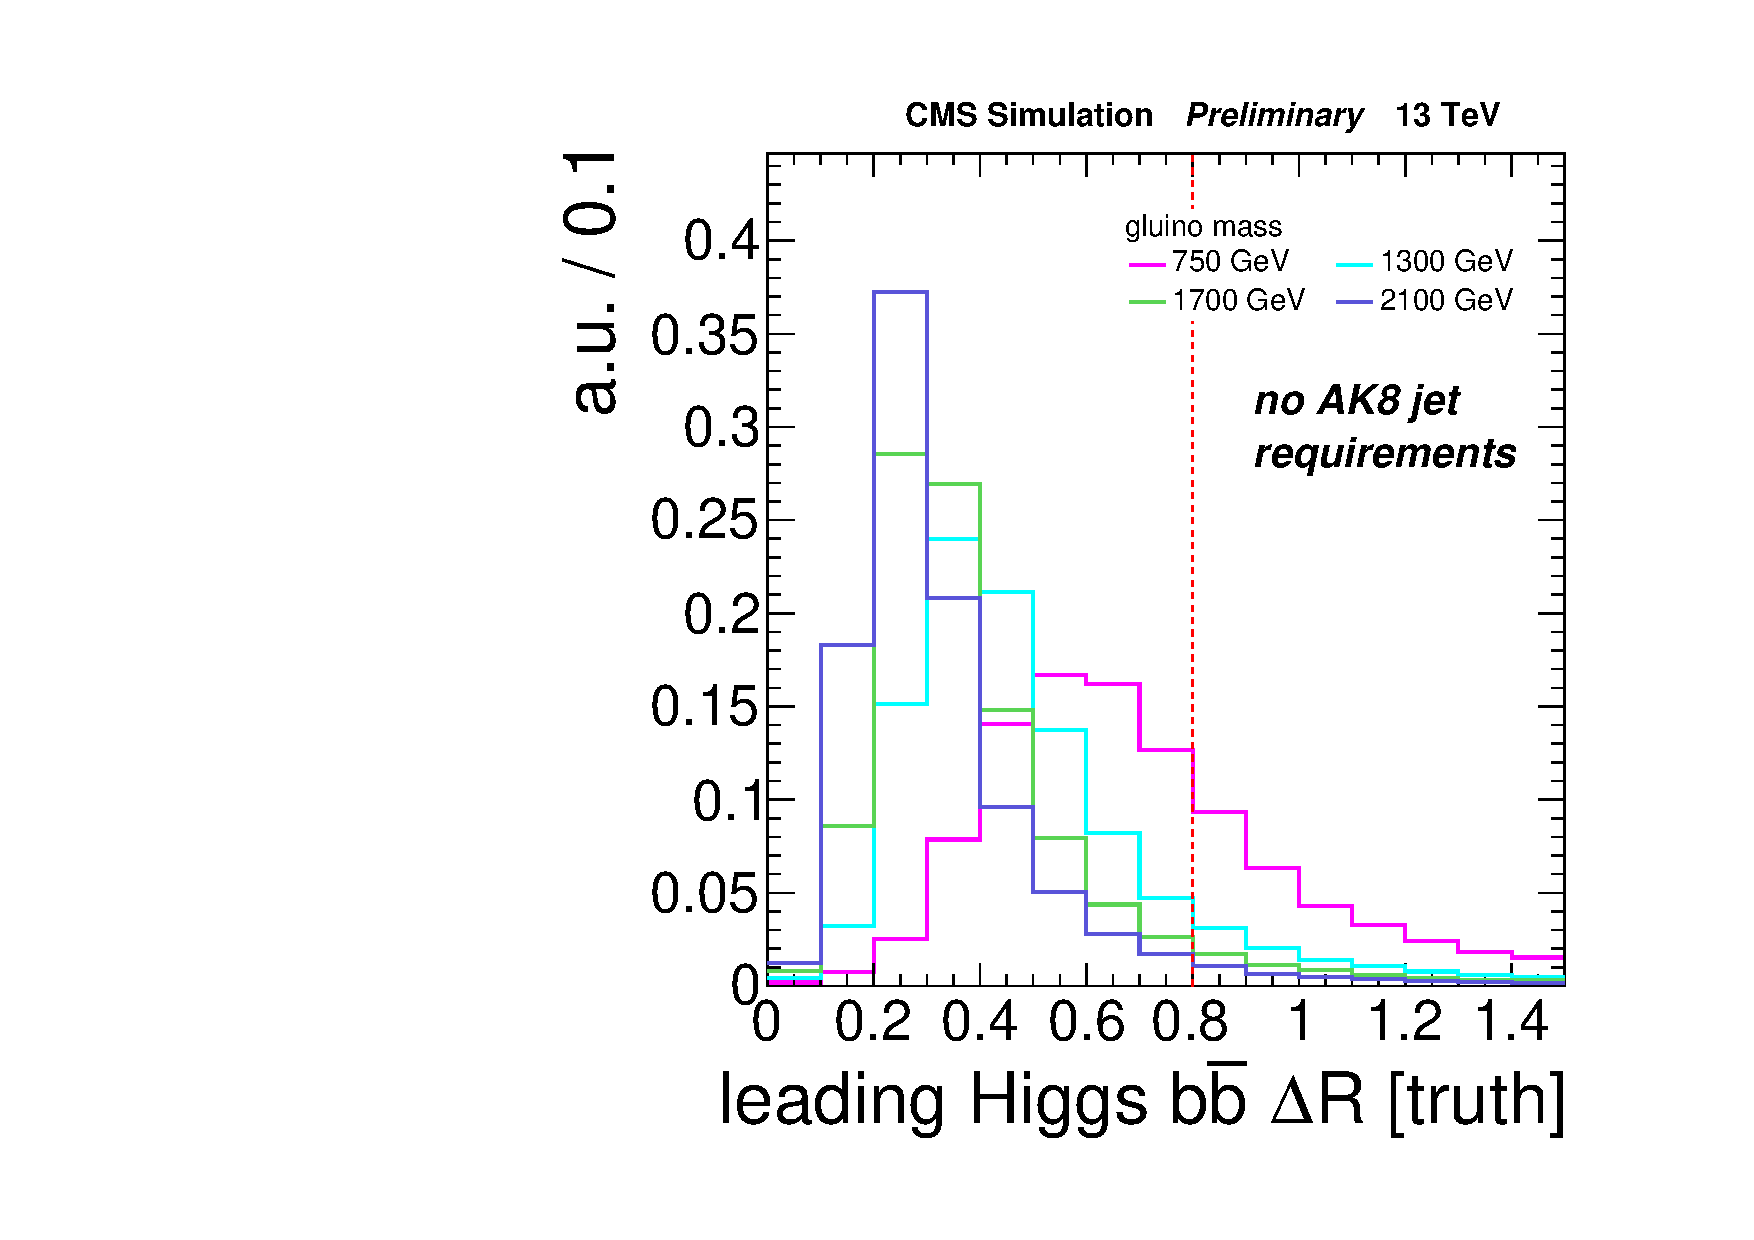
\includegraphics[width=0.425\linewidth]{figs/leadHiggsDr.pdf}\\
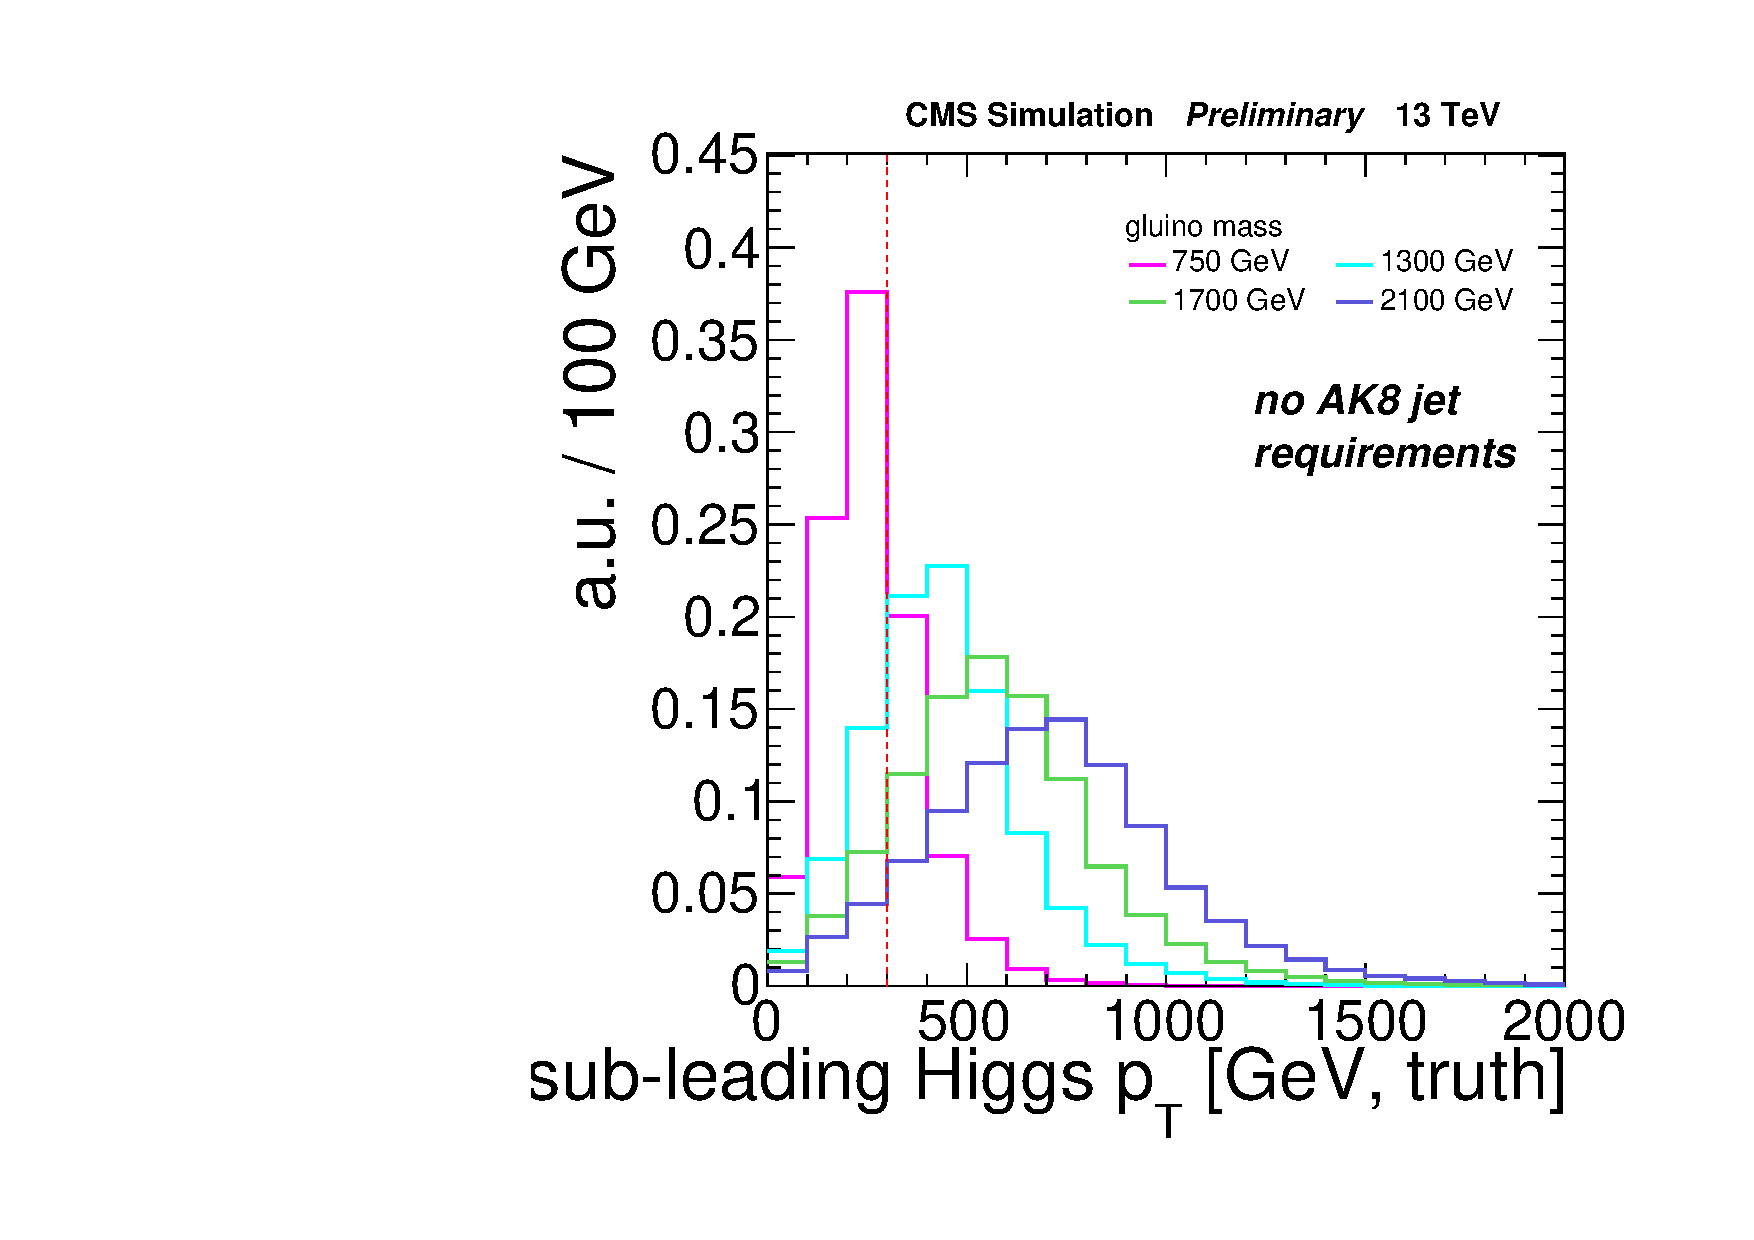
\includegraphics[width=0.425\linewidth]{figs/subleadHiggsPt.pdf}
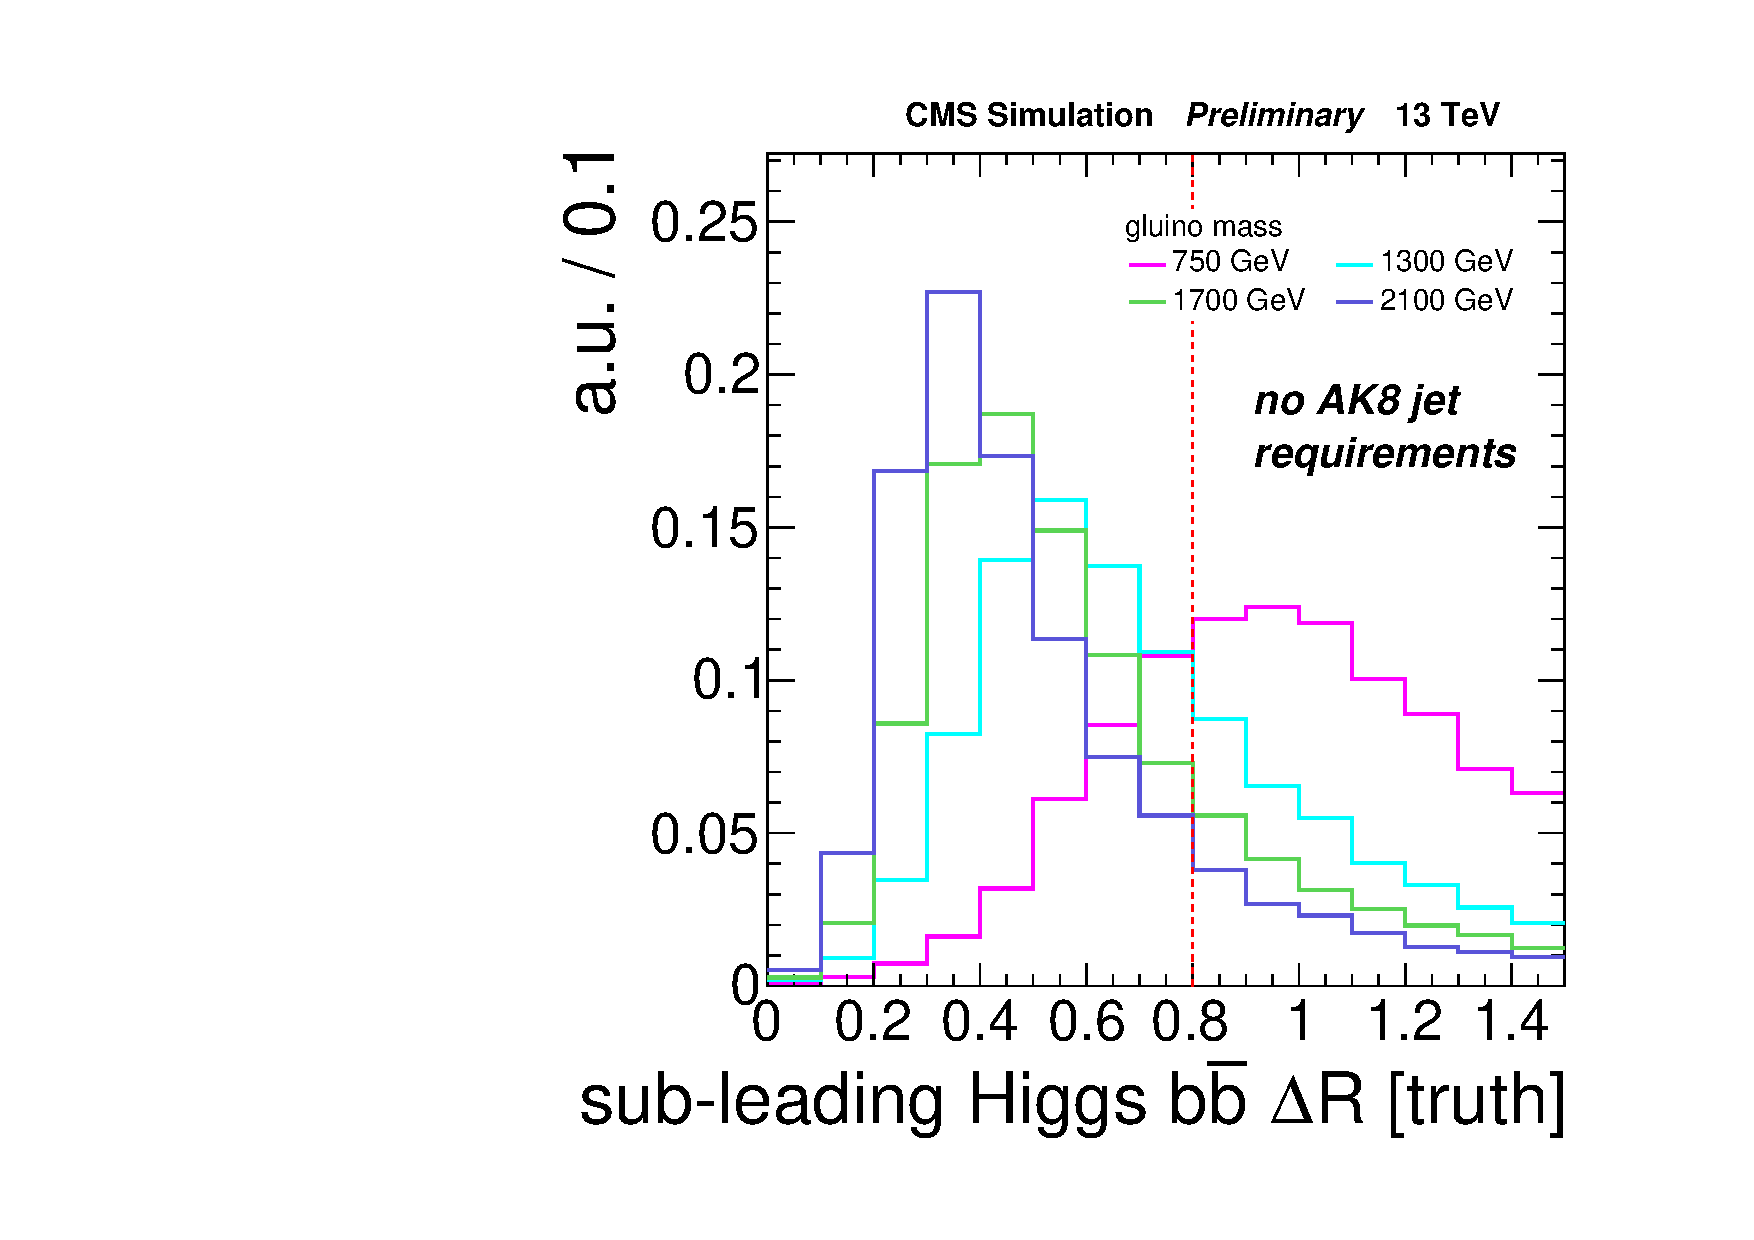
\includegraphics[width=0.425\linewidth]{figs/subleadHiggsDr.pdf}\\
\caption
[Generator level distributions for the H bosons in the T5HH model.]
{Generator level distributions for the highest (top row) and second highest (bottom row) \pt H boson in the T5HH model. The plot on the left shows the \pt of the H boson. The plot on right shows $\Delta R$ between the b-quark daughters - for large H \pt the daughters become collimated.}
\label{fig:GenHiggsBoost}
\end{figure}

\section{Event Binning \& Background Estimation}

The background estimation procedure makes use of what is known as an ``ABCD'' prediction in which the analysis phase space is divided into signal and sideband regions; scaling relations are applied to sideband yields to make predictions for the background in the signal regions. The events are categorized according to whether the two highest p$_{T}$ AK8 jets are a) in the signal or sideband mass region and b) have or have not been \bbbar tagged. A diagram of this partitioning is seen in Figure~\ref{fig:abcd}. An additional dimension is added by binning in \ptmiss: [300, 500 GeV], [500, 700 GeV], [700, $\infty$ GeV]. This additional binning, motivated by the \ptmiss distributions of Figure \ref{fig:met}, allows us to maximize sensitivity for both low and high \ptmiss signal. This gives a total of 2x3=6 signal and 4x3=12 sideband bins. The two signal regions A$_{1}$ and A$_{2}$ contain events with exactly one and exactly two jets being consistent with H/Z boson decay, respectively.

\begin{figure}
\centering
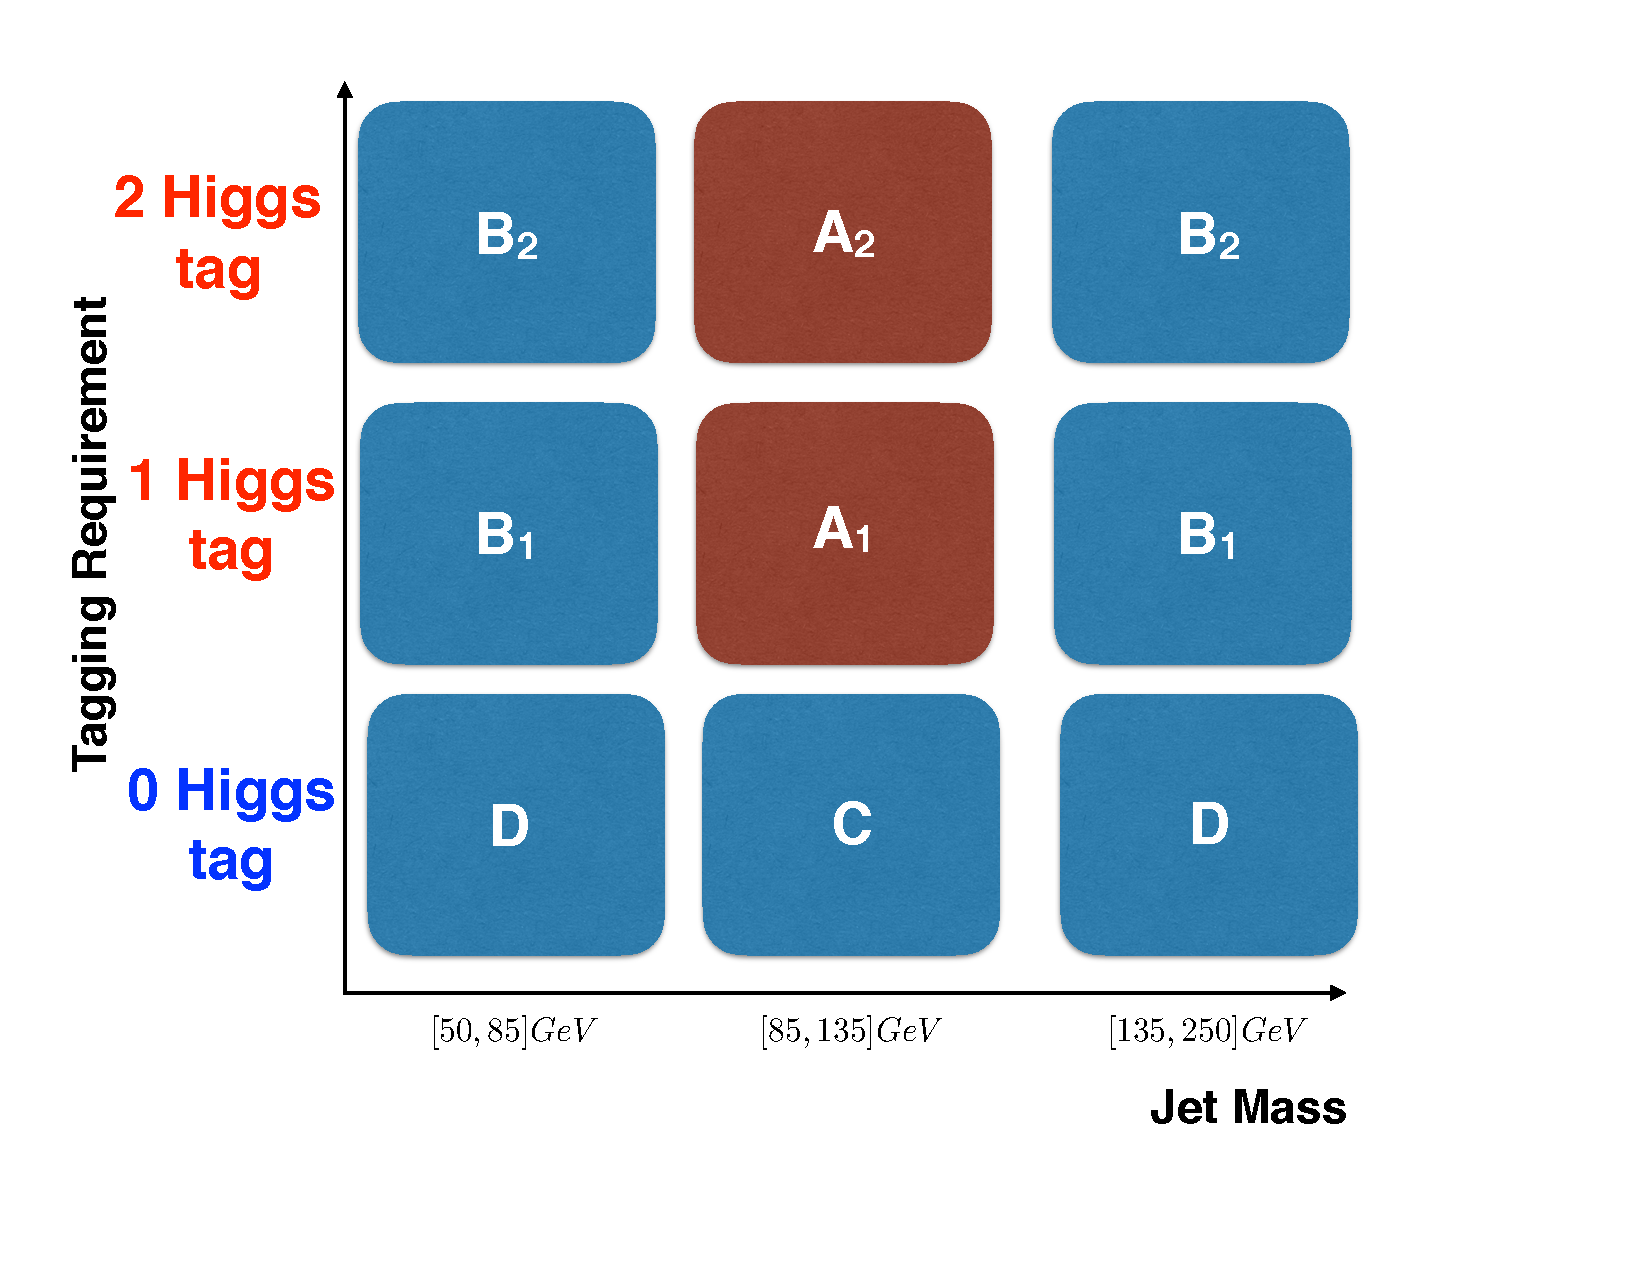
\includegraphics[width=0.6\textwidth]{figs/CMS-SUS-17-006_Figure-aux_002.pdf}
\caption[Partitioning of the signal and sideband regions for event binning.]{Partitioning of the signal and sideband regions for event binning. Additional binning in \ptmiss brings the total to 6x3=18.}
\label{fig:abcd}
\end{figure}

\begin{figure}
\centering
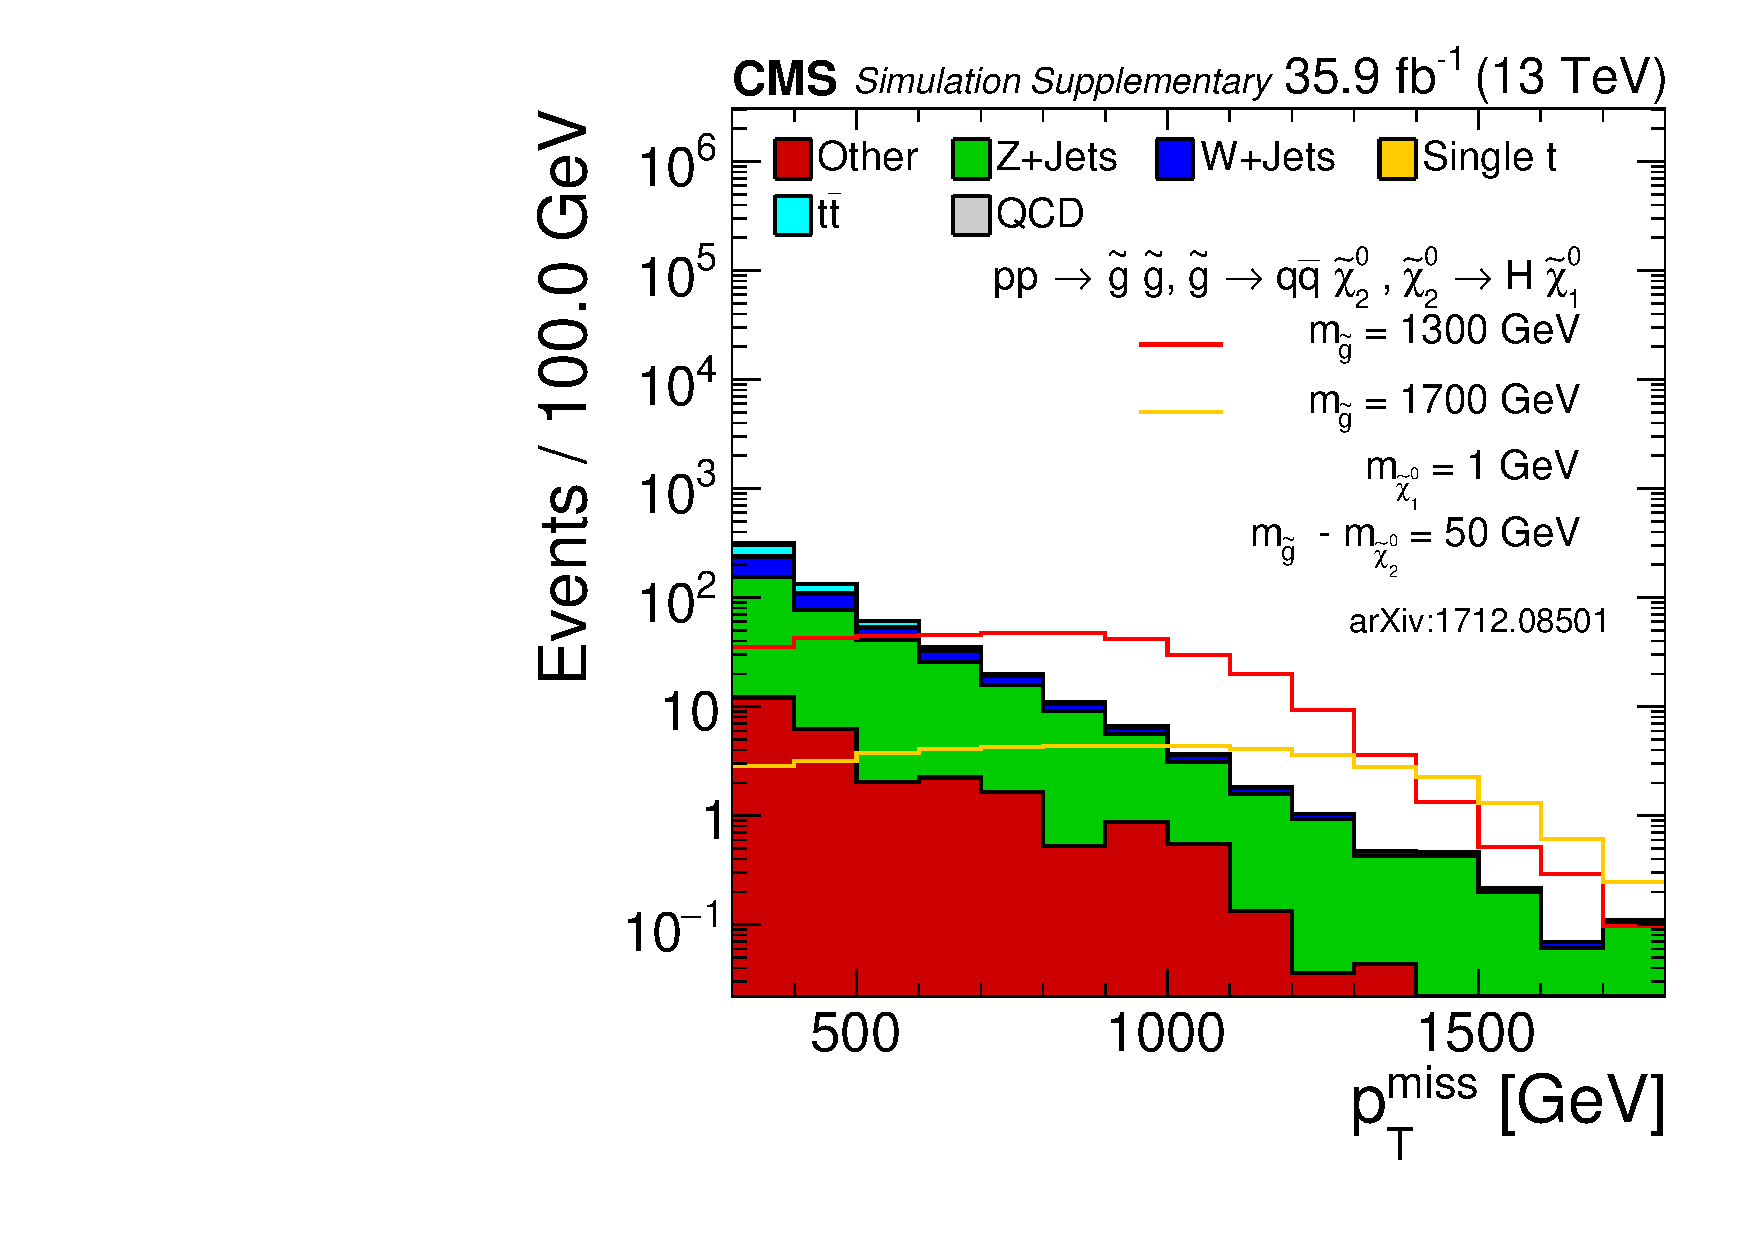
\includegraphics[width=0.425\textwidth]{figs/MET_baseline_LogY.pdf}
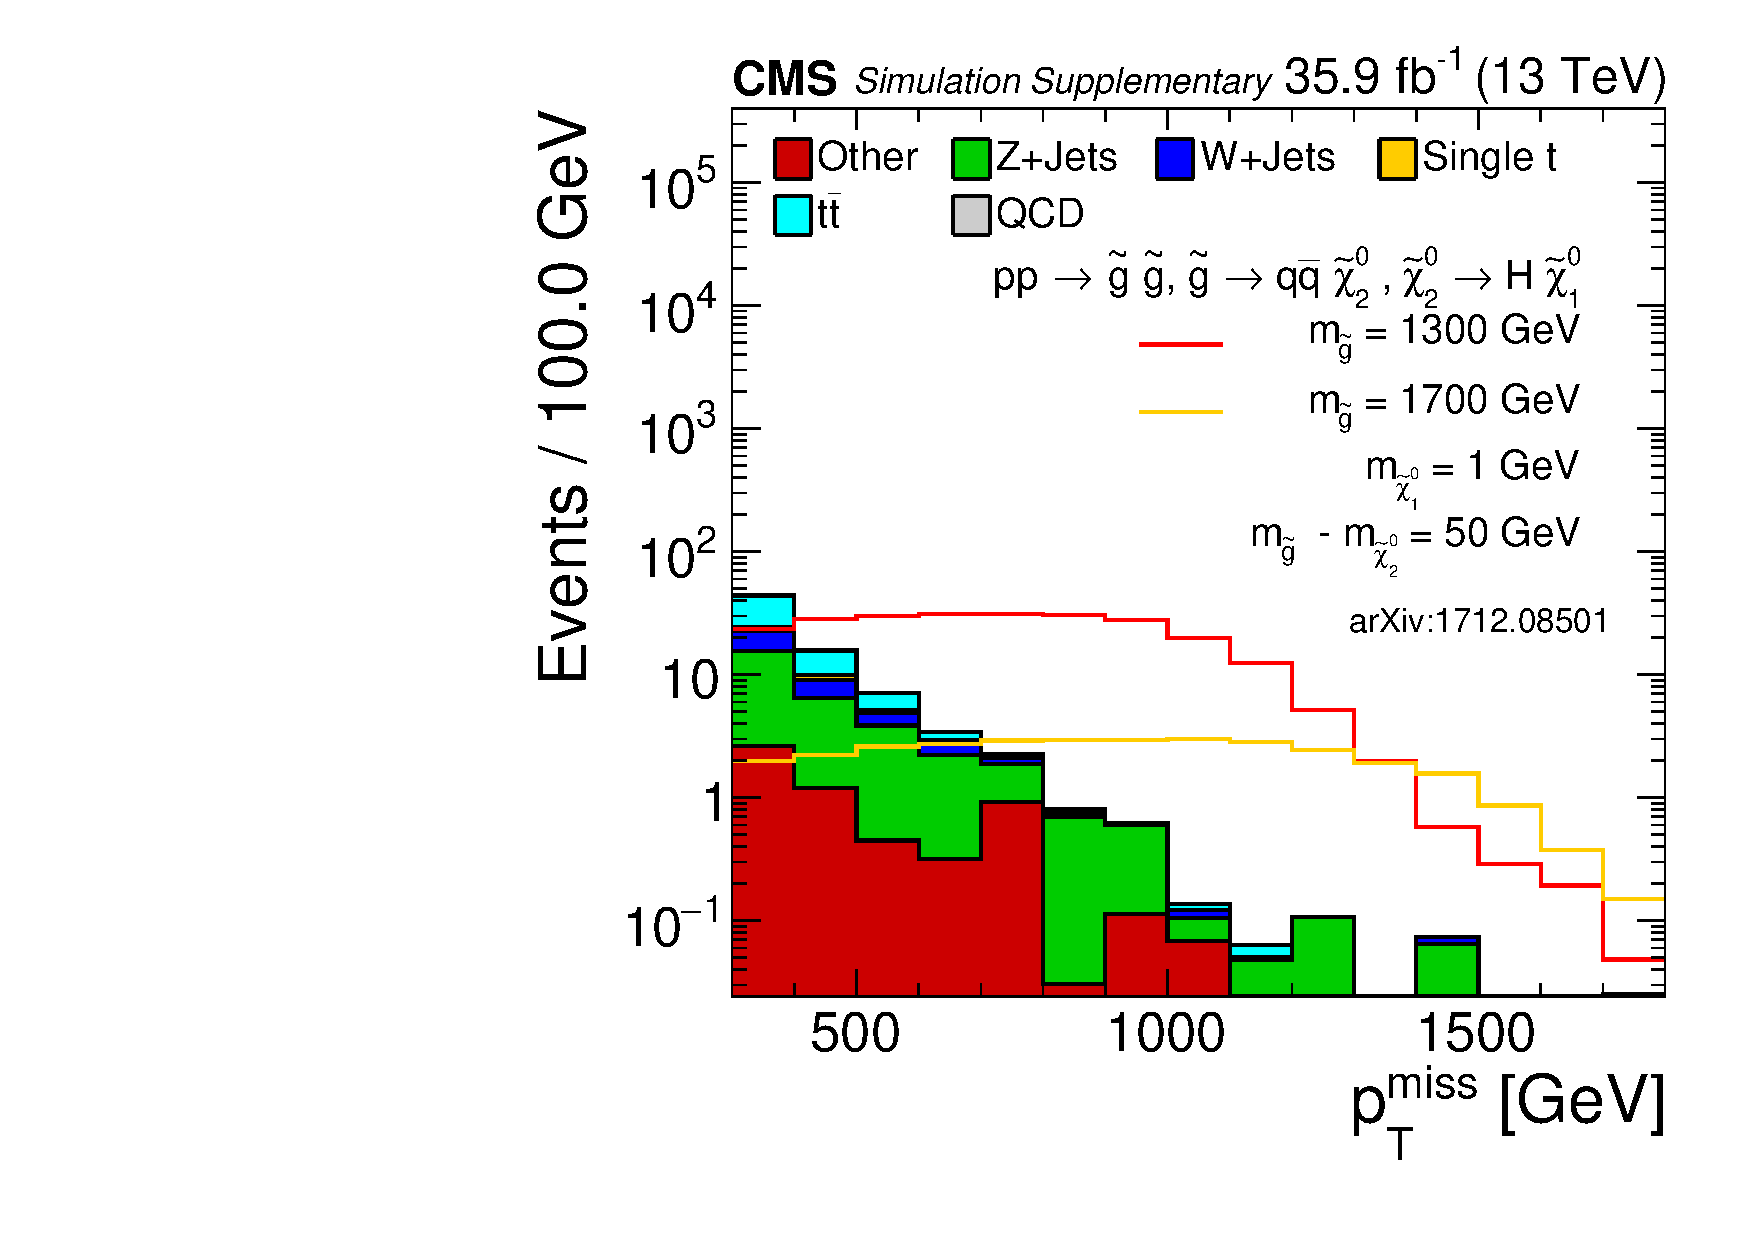
\includegraphics[width=0.425\textwidth]{figs/MET_singleHiggsTag_LogY.pdf}
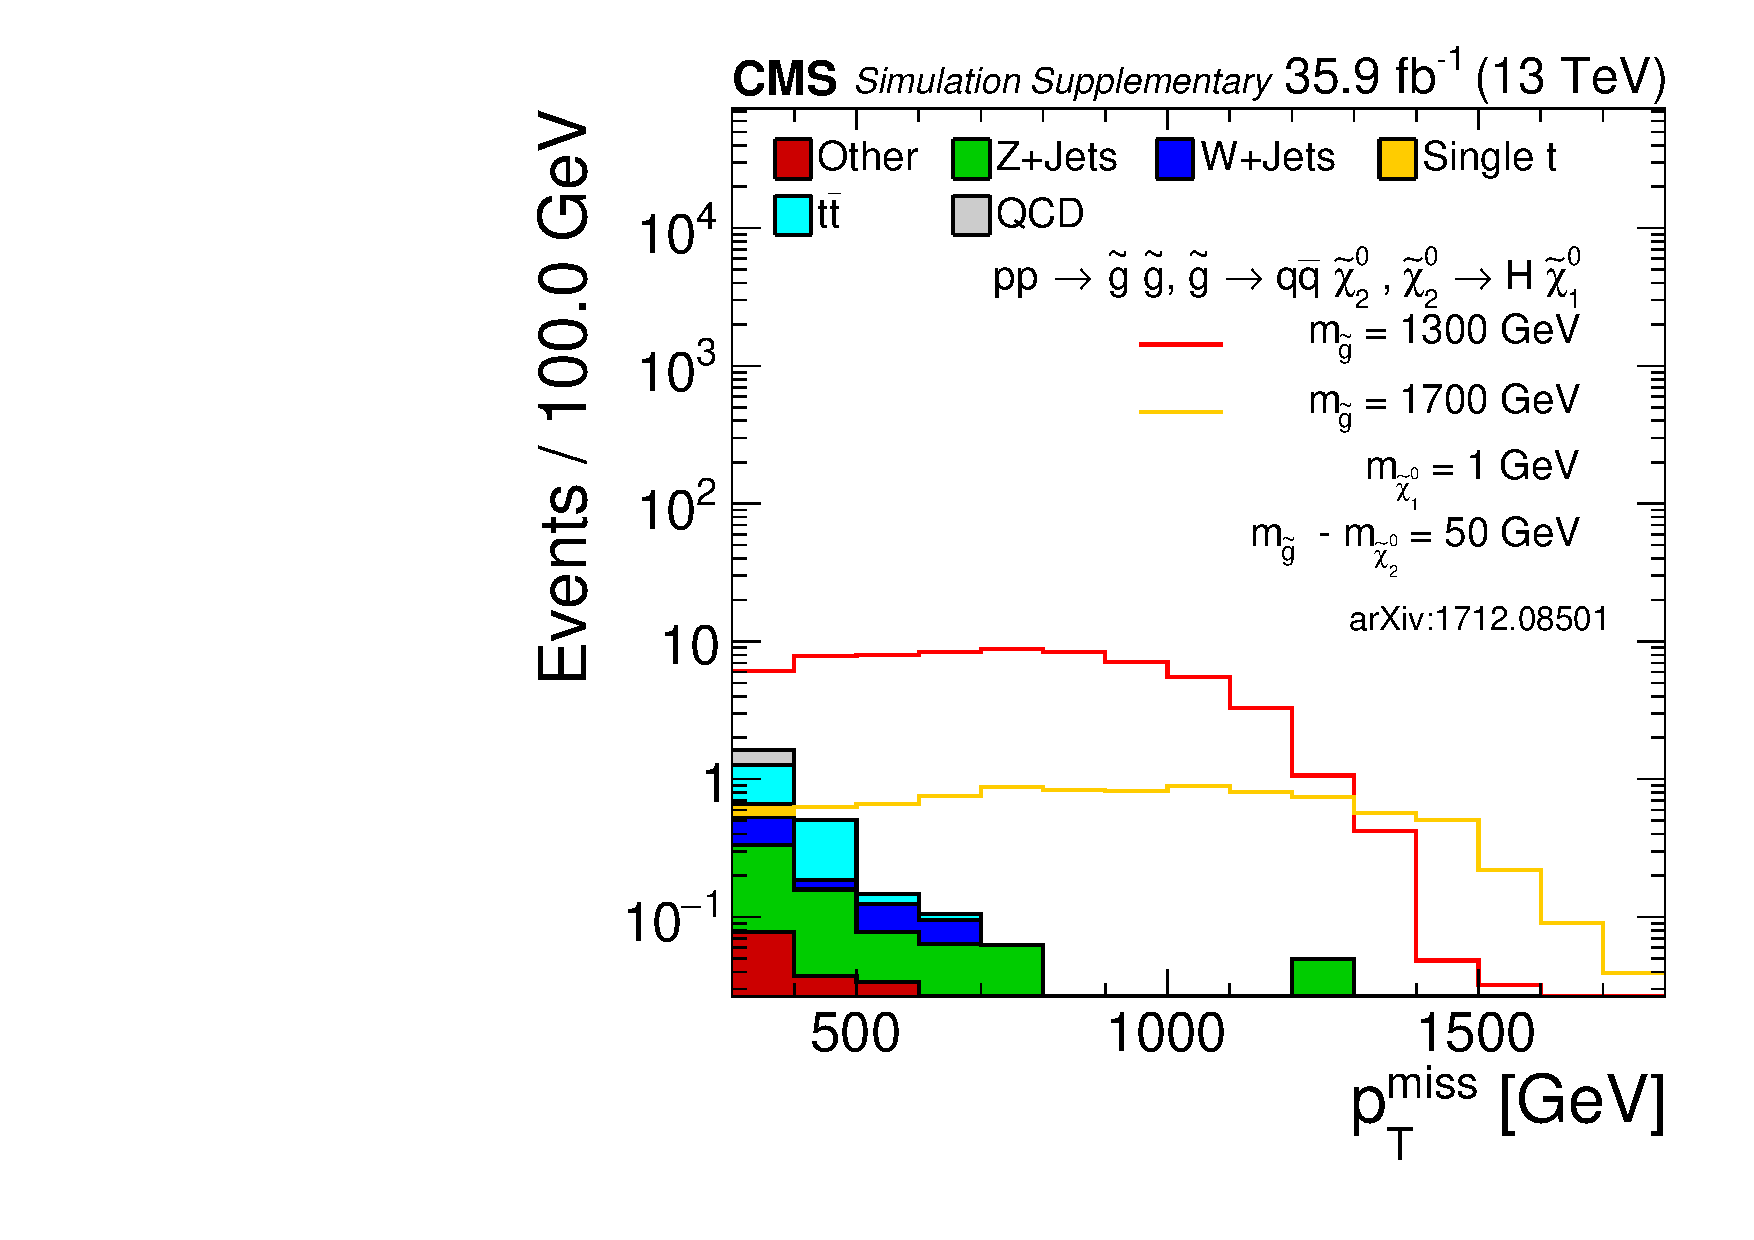
\includegraphics[width=0.425\textwidth]{figs/MET_doubleHiggsTag_LogY.pdf}

\includegraphics[width=0.425\textwidth]{figs/blankcanvas.pdf}
\caption[MC distributions of \ptmiss after baseline selection.]{MC distributions of \ptmiss after baseline selection. The top right plot shows the single H-tagged region $A_{1}$, the bottom left plot shows the double H-tagged region $A_{2}$.}
\label{fig:met}
\end{figure}

Assuming that there is no correlation between the jet mass and the \bbbar-tagging one would expect that:

\begin{equation}
\frac{A_{1}}{B_{1}} = \frac{A_{2}}{B_{2}} = \frac{C}{D}
\end{equation}

Rearranging this gives a prediction for the events in the signal regions

\begin{equation}
\mathrm{A}_{1, 2}^{\mathrm{predicted}} = \left( \mathrm{B}_{1, 2} \cdot \frac{\mathrm{C}}{\mathrm{D}}\right)^{\mathrm{observed}}
\end{equation}

The expected \ptmiss distribution from simulation is seen in the stacked histograms of Figure~\ref{fig:MCclosure}. The prediction using the ABCD method on the same simulated samples is seen in the red hash. The performance of the method within simulation can be determined by dividing the true content in the signal region with the prediction. This ratio, denoted $\kappa$, is seen in the bottom panel of Figure~\ref{fig:MCclosure}. $\kappa=1$ represents perfect modeling. As will be discussed in Section~\ref{sec:kappa}, $\kappa$ is used as a correction in the background estimation procedure.

\begin{figure}
\centering
\begin{subfigure}[b]{0.425\textwidth}
\centering
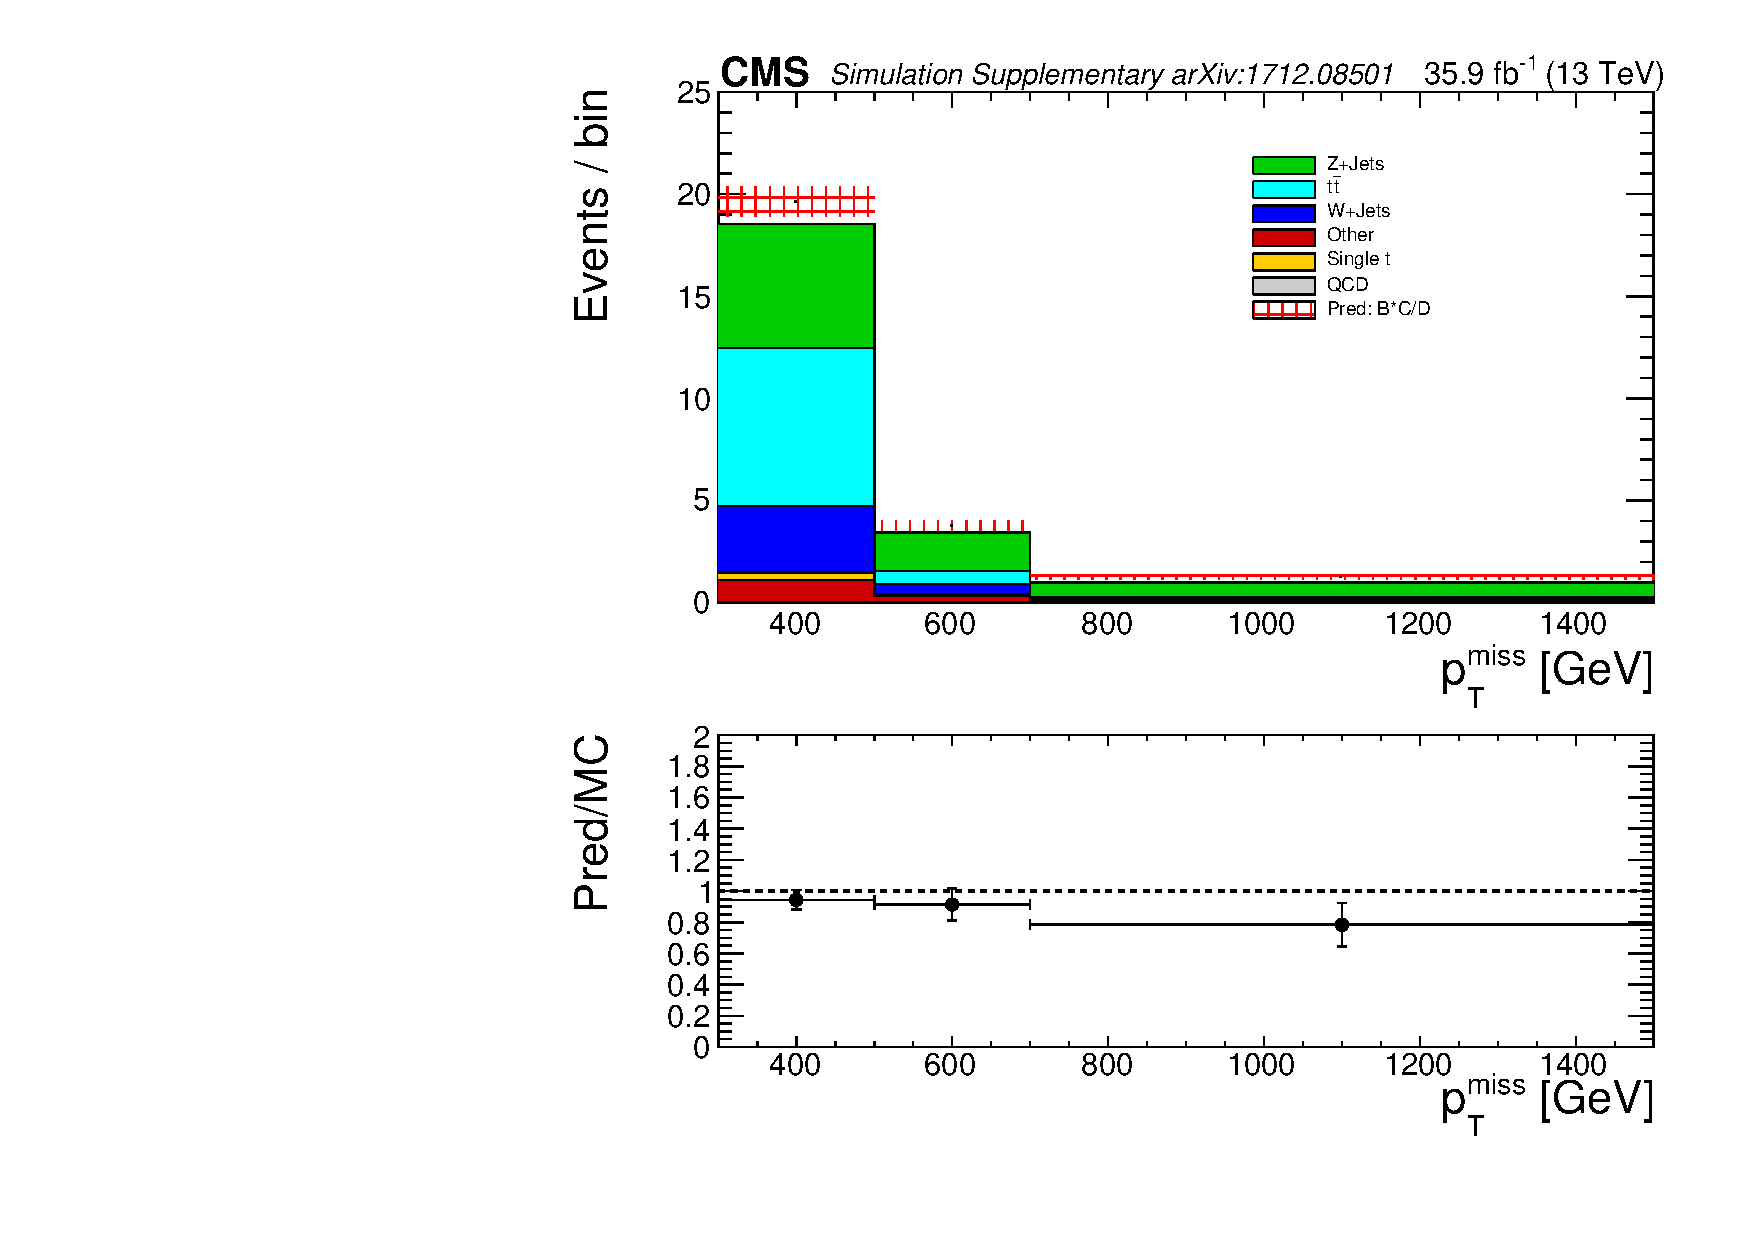
\includegraphics[trim={5px 5px 5px 5px},clip,width=0.95\textwidth]{figs/MCclosure_singleHiggsRegionTotal.pdf}
\caption{The single Higgs tag region (A$_{1}$).}
\end{subfigure}
\begin{subfigure}[b]{0.425\textwidth}
\centering
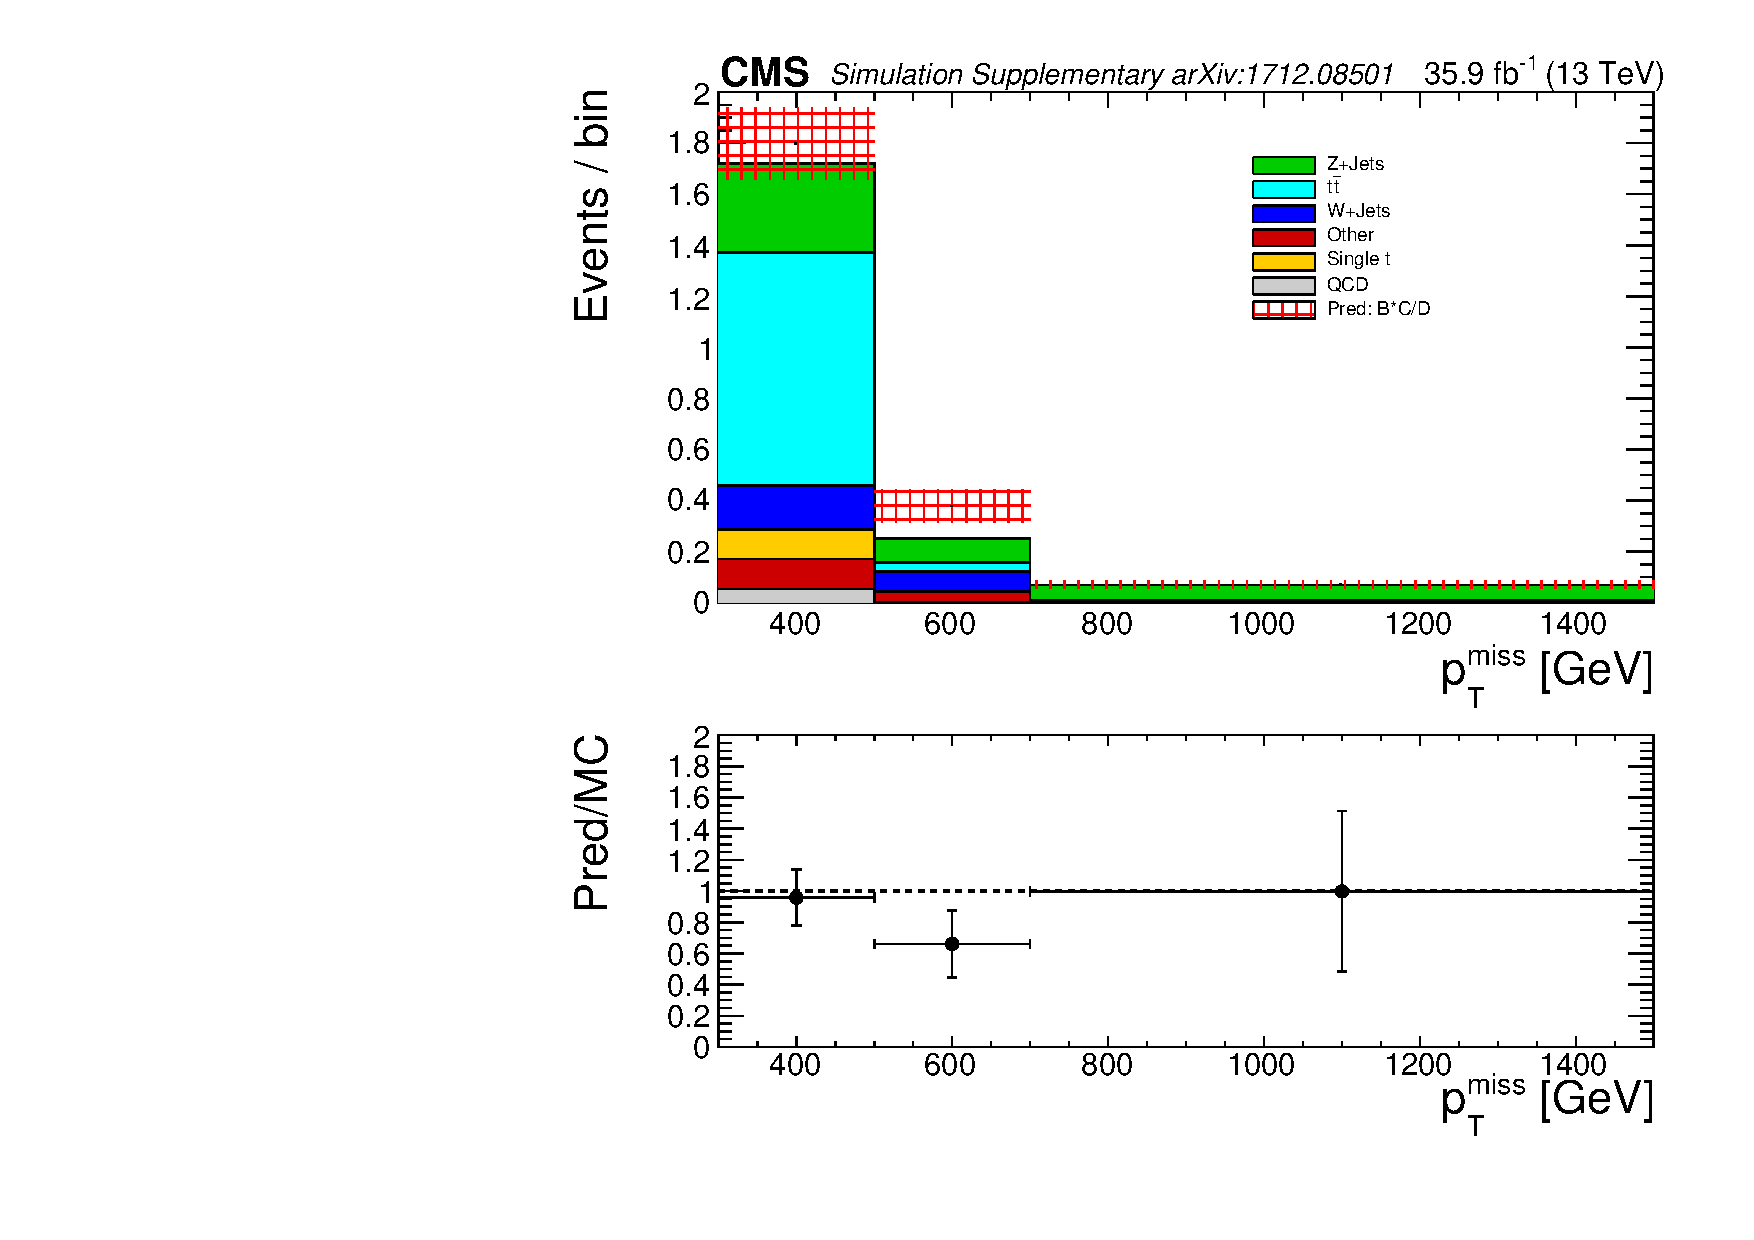
\includegraphics[trim={5px 5px 5px 5px},clip,width=0.95\textwidth]{figs/MCclosure_doubleHiggsRegionTotal.pdf} 
\caption{The double Higgs tag region (A$_{2}$).}
\end{subfigure}
\caption{\ptmiss distributions and predictions in the signal regions using simulation only.}
\label{fig:MCclosure}
\end{figure}

\subsection{Control Regions within Data}
\label{sec:smbkg}

%\begin{figure}
%\centering
%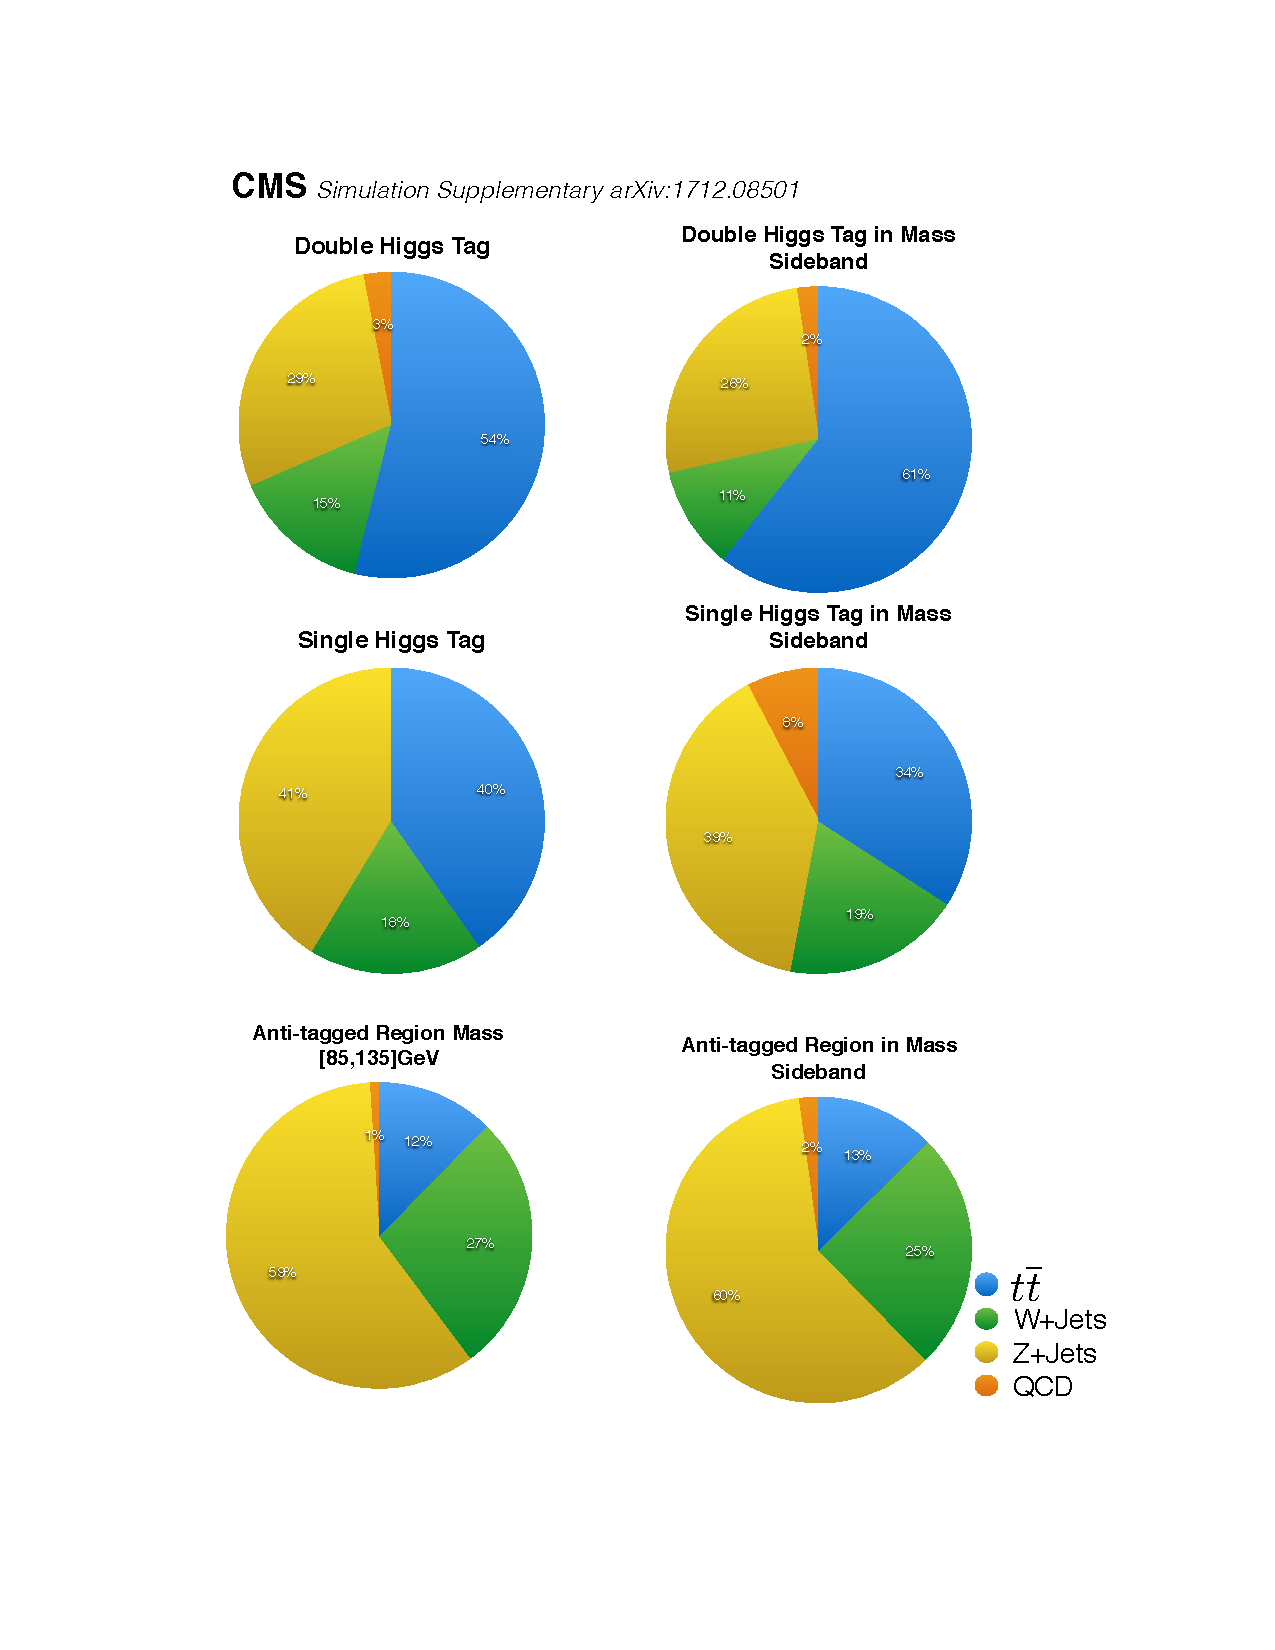
\includegraphics[width=0.5\textwidth]{figs/CMS-SUS-17-006_Figure-aux_003.pdf}
%\caption{The fractional composition of expected SM backgrounds in the 6 analysis regions.}
%\label{fig:bkgfrac}
%\end{figure}

In order to study the expected backgrounds in data ($Z\rightarrow\nu\bar{\nu}$, $\mathrm{t}\bar{\mathrm{t}} \rightarrow \ell \nu q q'$ $W\rightarrow\ell\nu$, QCD), we define three control regions which are enhanced in processes representative to the background. The event selection is the same as applied to the nominal signal and sideband regions, but with some defining orthogonal condition:

\begin{itemize}

\item A control region with a single photon. For high-$p_{T}$, photons and Z bosons are both massless, neutral, gauge bosons and therefore their kinematics are expected to be similar.  ``Artificial'' removal of the photon from the reconstruction (i.e. ignore its calorimeter deposit) results in event topologies phenomenologically similar to $Z\rightarrow\nu\bar{\nu}$.

\item A control region with a single lepton. The topology of events from direct W or top quark production is the same regardless if the electron or muon is identified as such. 

\item A control region defined by the logical inversion of the low-$\Delta\phi$ cut. This explicitly selects events in which the AK4 jet momentum was likely under-measured, resulting in close alignment with \ptmiss.

\end{itemize}

As they are orthogonal to the analysis region, we are able to test the validity of the background estimation technique independently \textbf{within} each of the three control regions. By comparing the prediction of the yields using the ABCD method with those observed, the validity of the technique can be verified for that particular background category. The comparisons for the single-photon, single-lepton and low-$\Delta\phi$ control regions can be seen in Figure~\ref{fig:closure}. $\kappa$ in the bottom panel is defined as the ratio of the true event yield to the prediction. $\kappa=1$ represents the case in which the prediction perfectly matches the observation. These comparisons are used for commissioning of the background estimation technique only.

\begin{figure}
\centering
\begin{subfigure}[b]{0.425\textwidth}
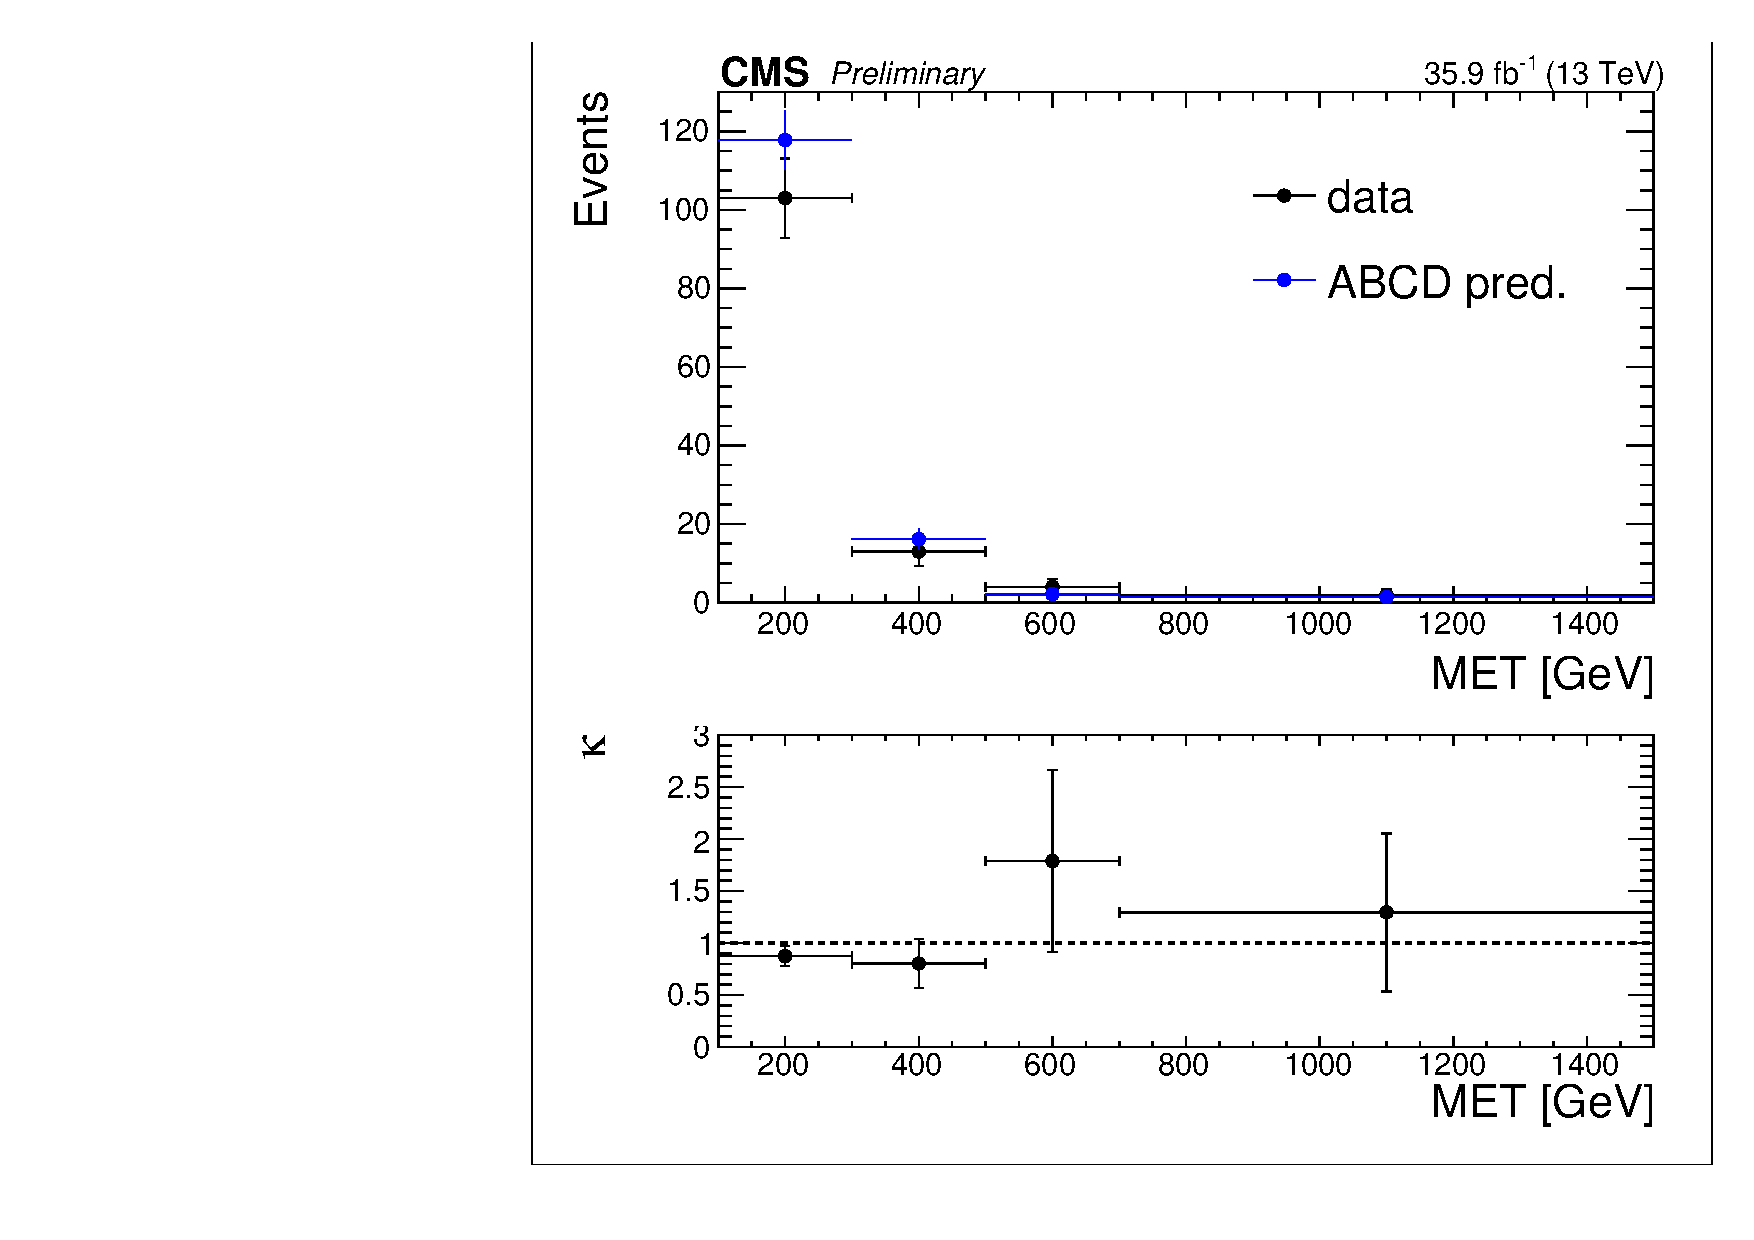
\includegraphics[trim={5px 5px 5px 5px},clip,width=0.95\textwidth]{figs/dataClosure_single-tagSR_photon.pdf}
\caption{single photon A$_{1}$}
\end{subfigure}
\begin{subfigure}[b]{0.425\textwidth}
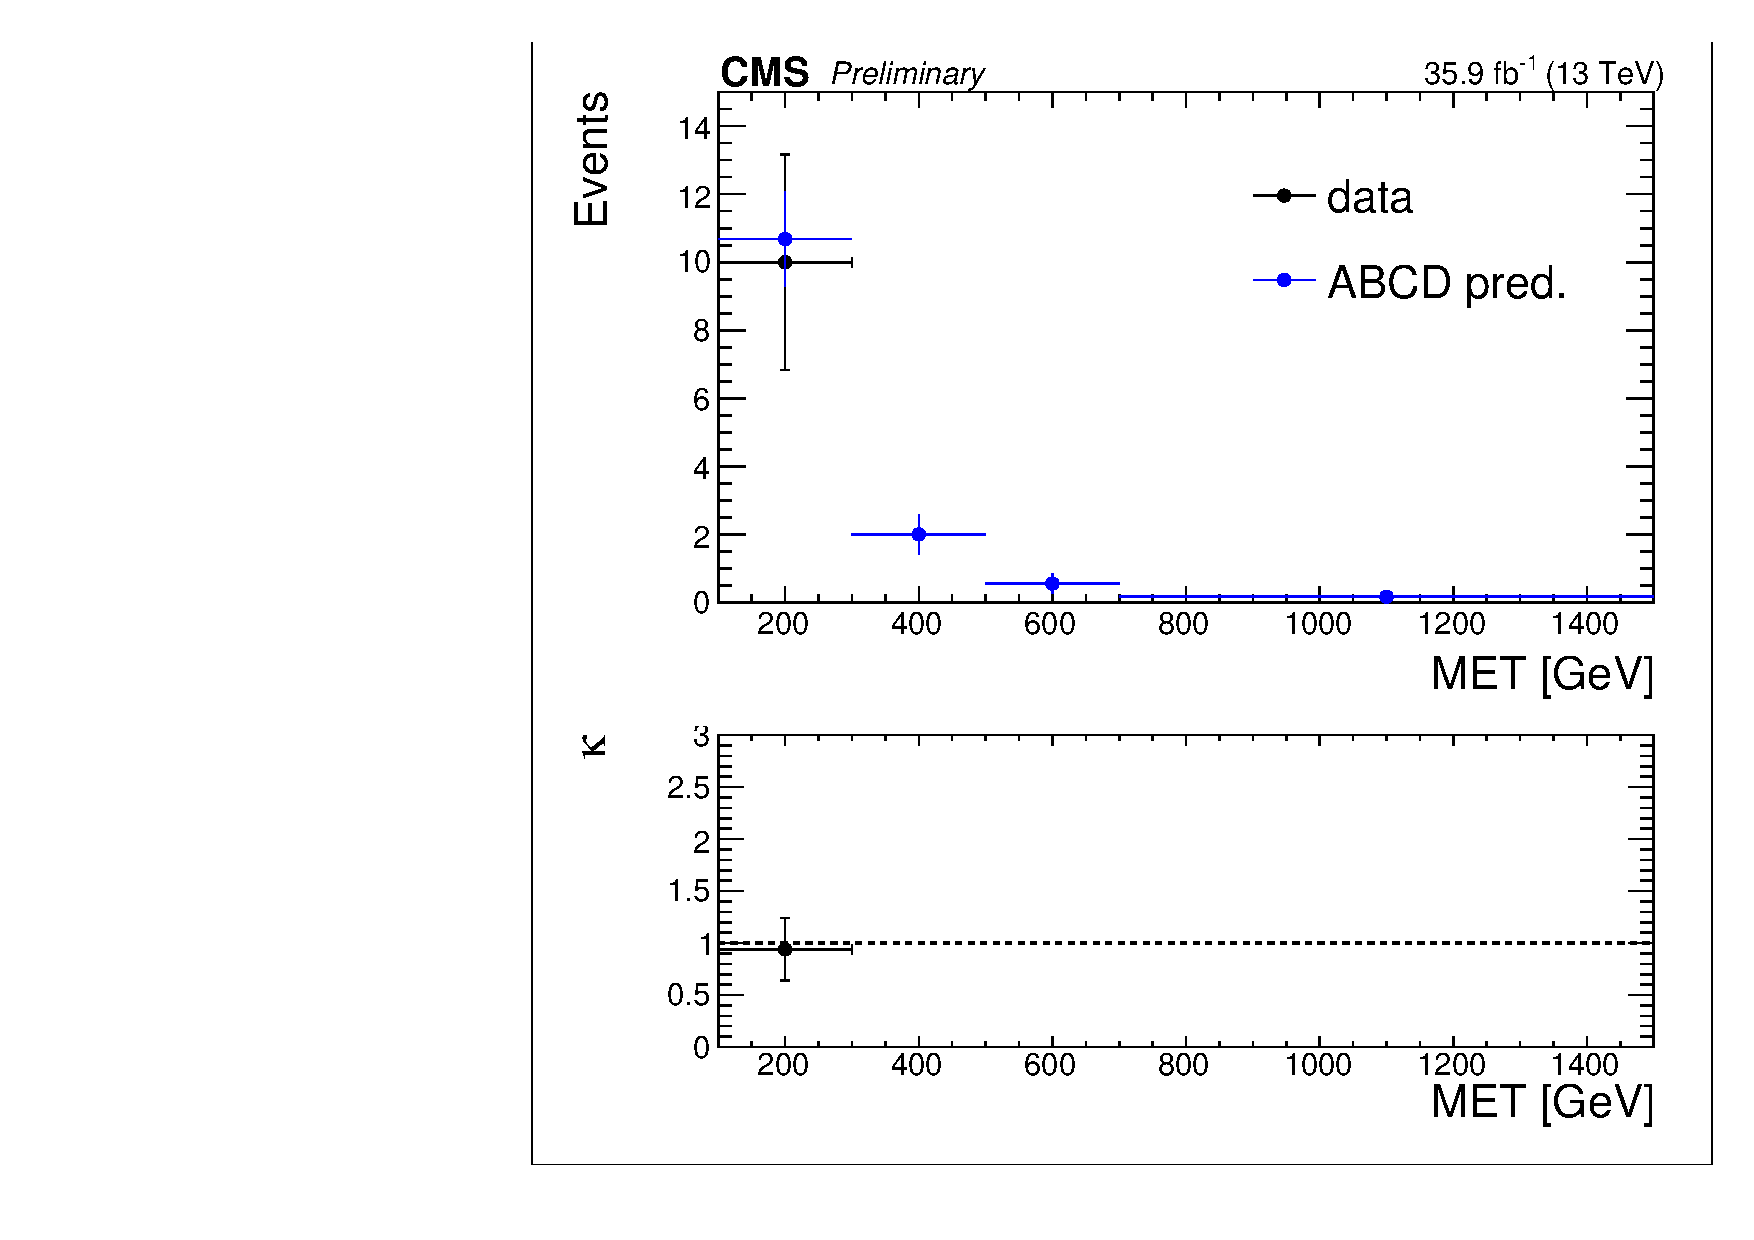
\includegraphics[trim={5px 5px 5px 5px},clip,width=0.95\textwidth]{figs/dataClosure_double-tagSR_photon.pdf} 
\caption{single photon A$_{2}$}
\end{subfigure}
\vspace{5mm}
\\
\begin{subfigure}[b]{0.425\textwidth}
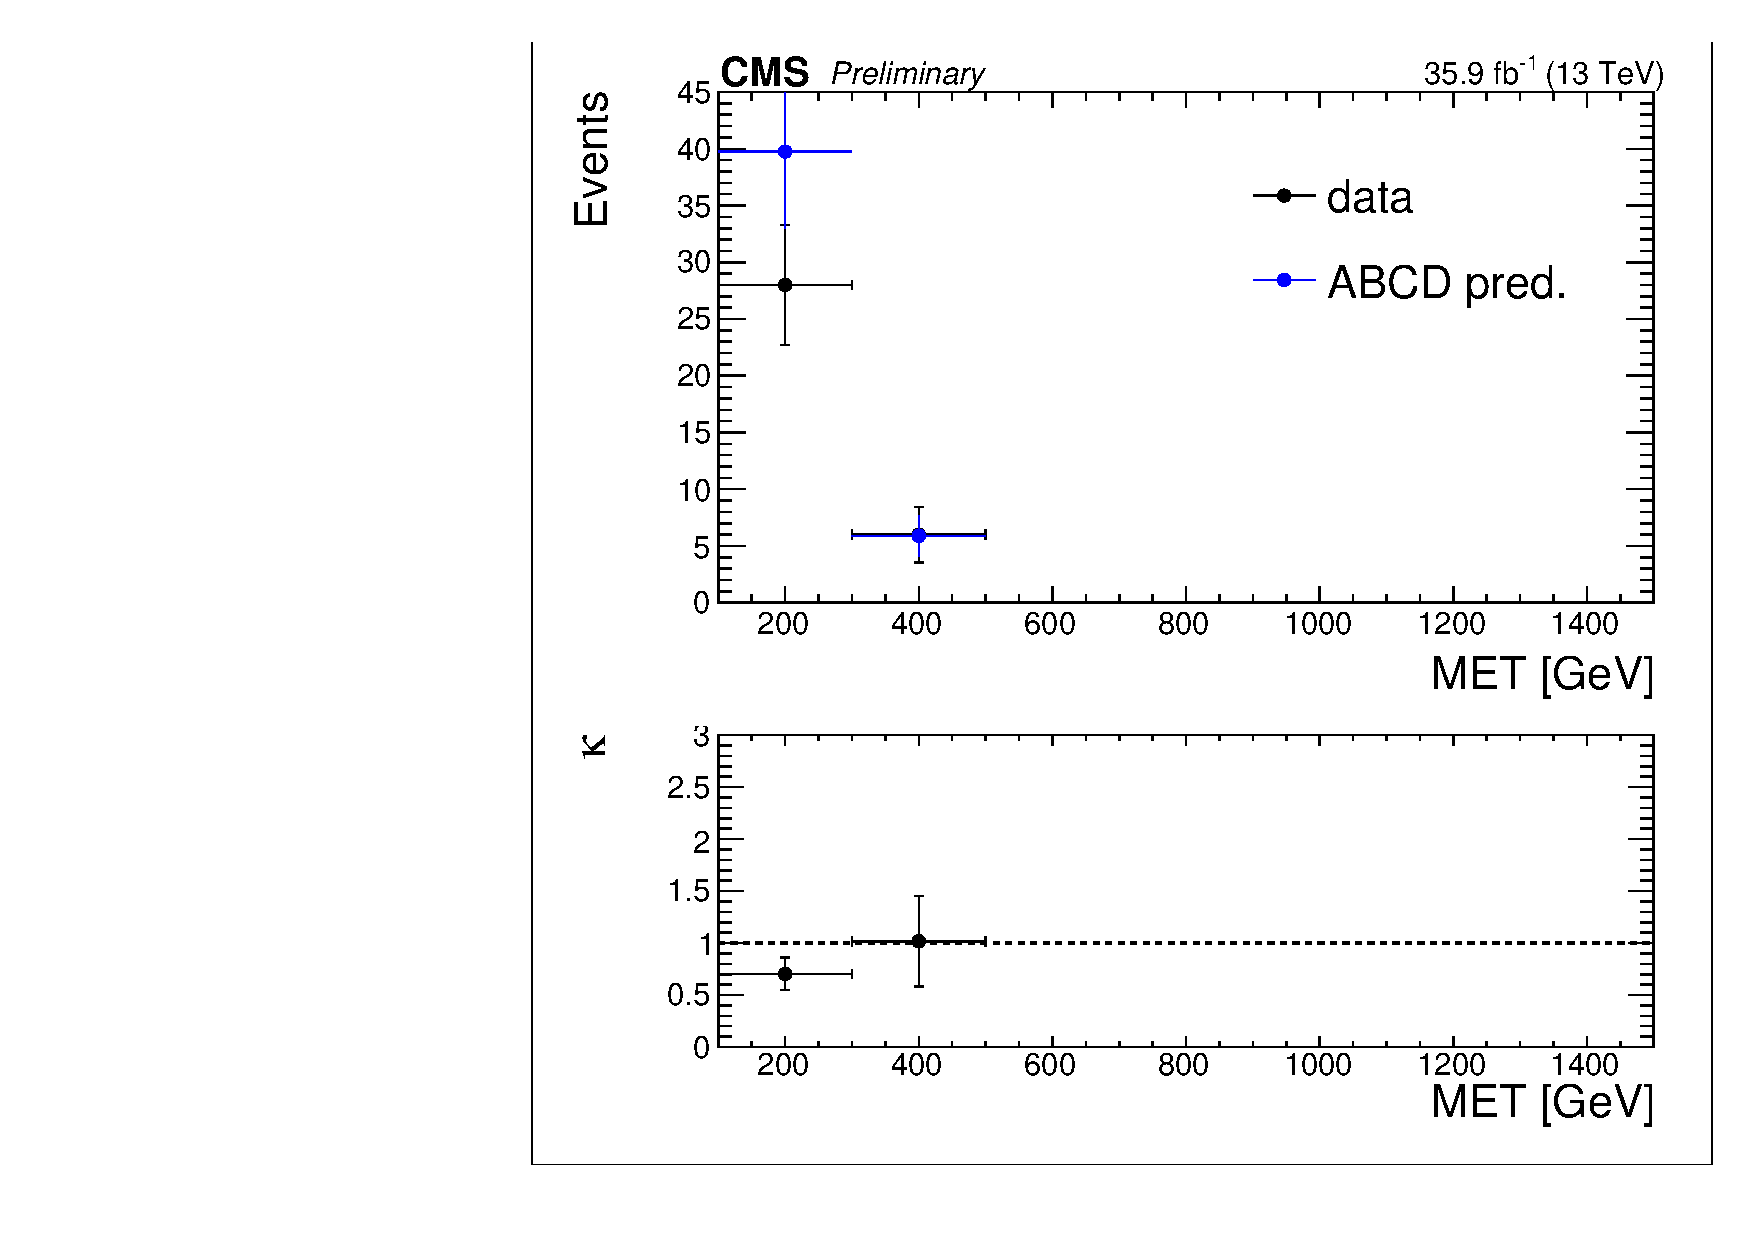
\includegraphics[trim={5px 5px 5px 5px},clip,width=0.95\textwidth]{figs/dataClosure_single-tagSR_singleLep.pdf} 
\caption{single lepton A$_{1}$}
\end{subfigure}
\begin{subfigure}[b]{0.425\textwidth}
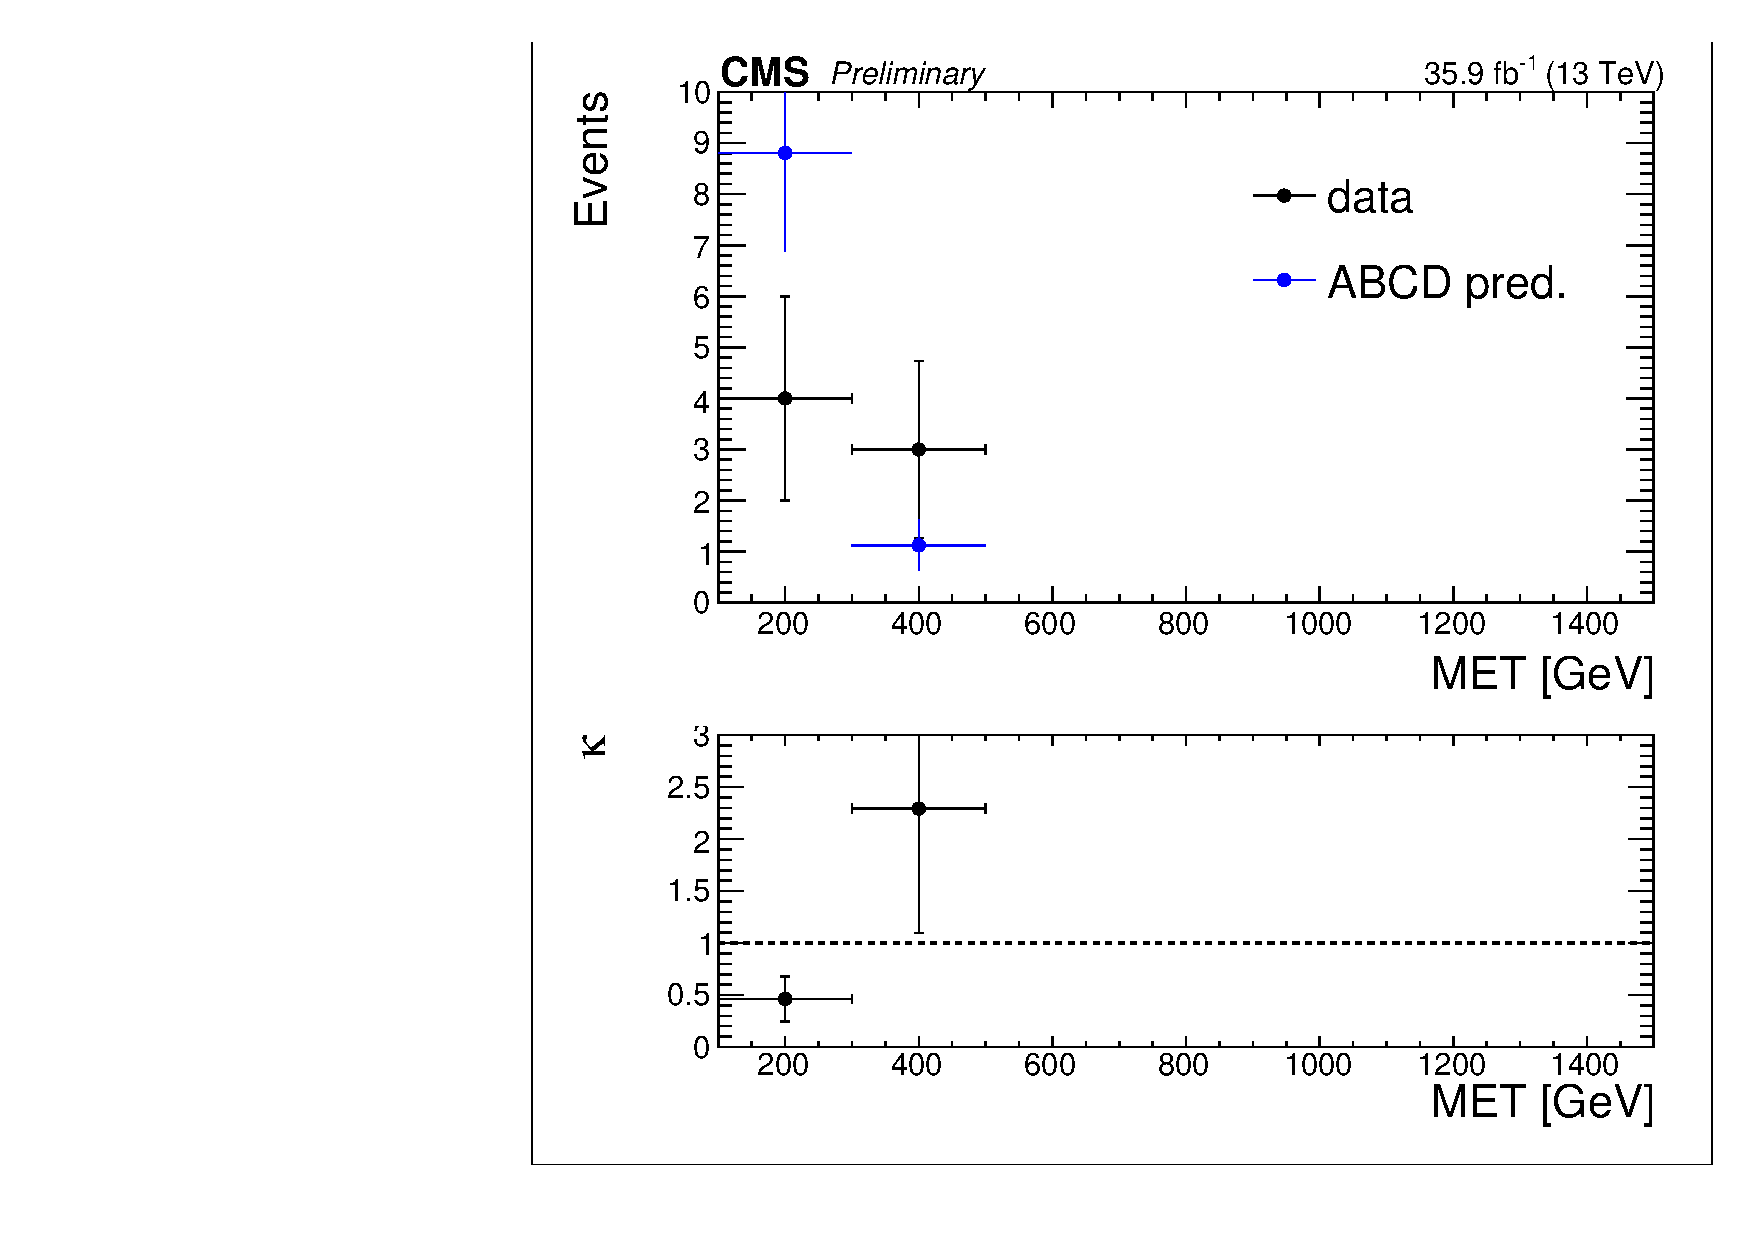
\includegraphics[trim={5px 5px 5px 5px},clip,width=0.95\textwidth]{figs/dataClosure_double-tagSR_singleLep.pdf} 
\caption{single lepton A$_{2}$}
\end{subfigure}
\vspace{5mm}
\\
\begin{subfigure}[b]{0.42\textwidth}
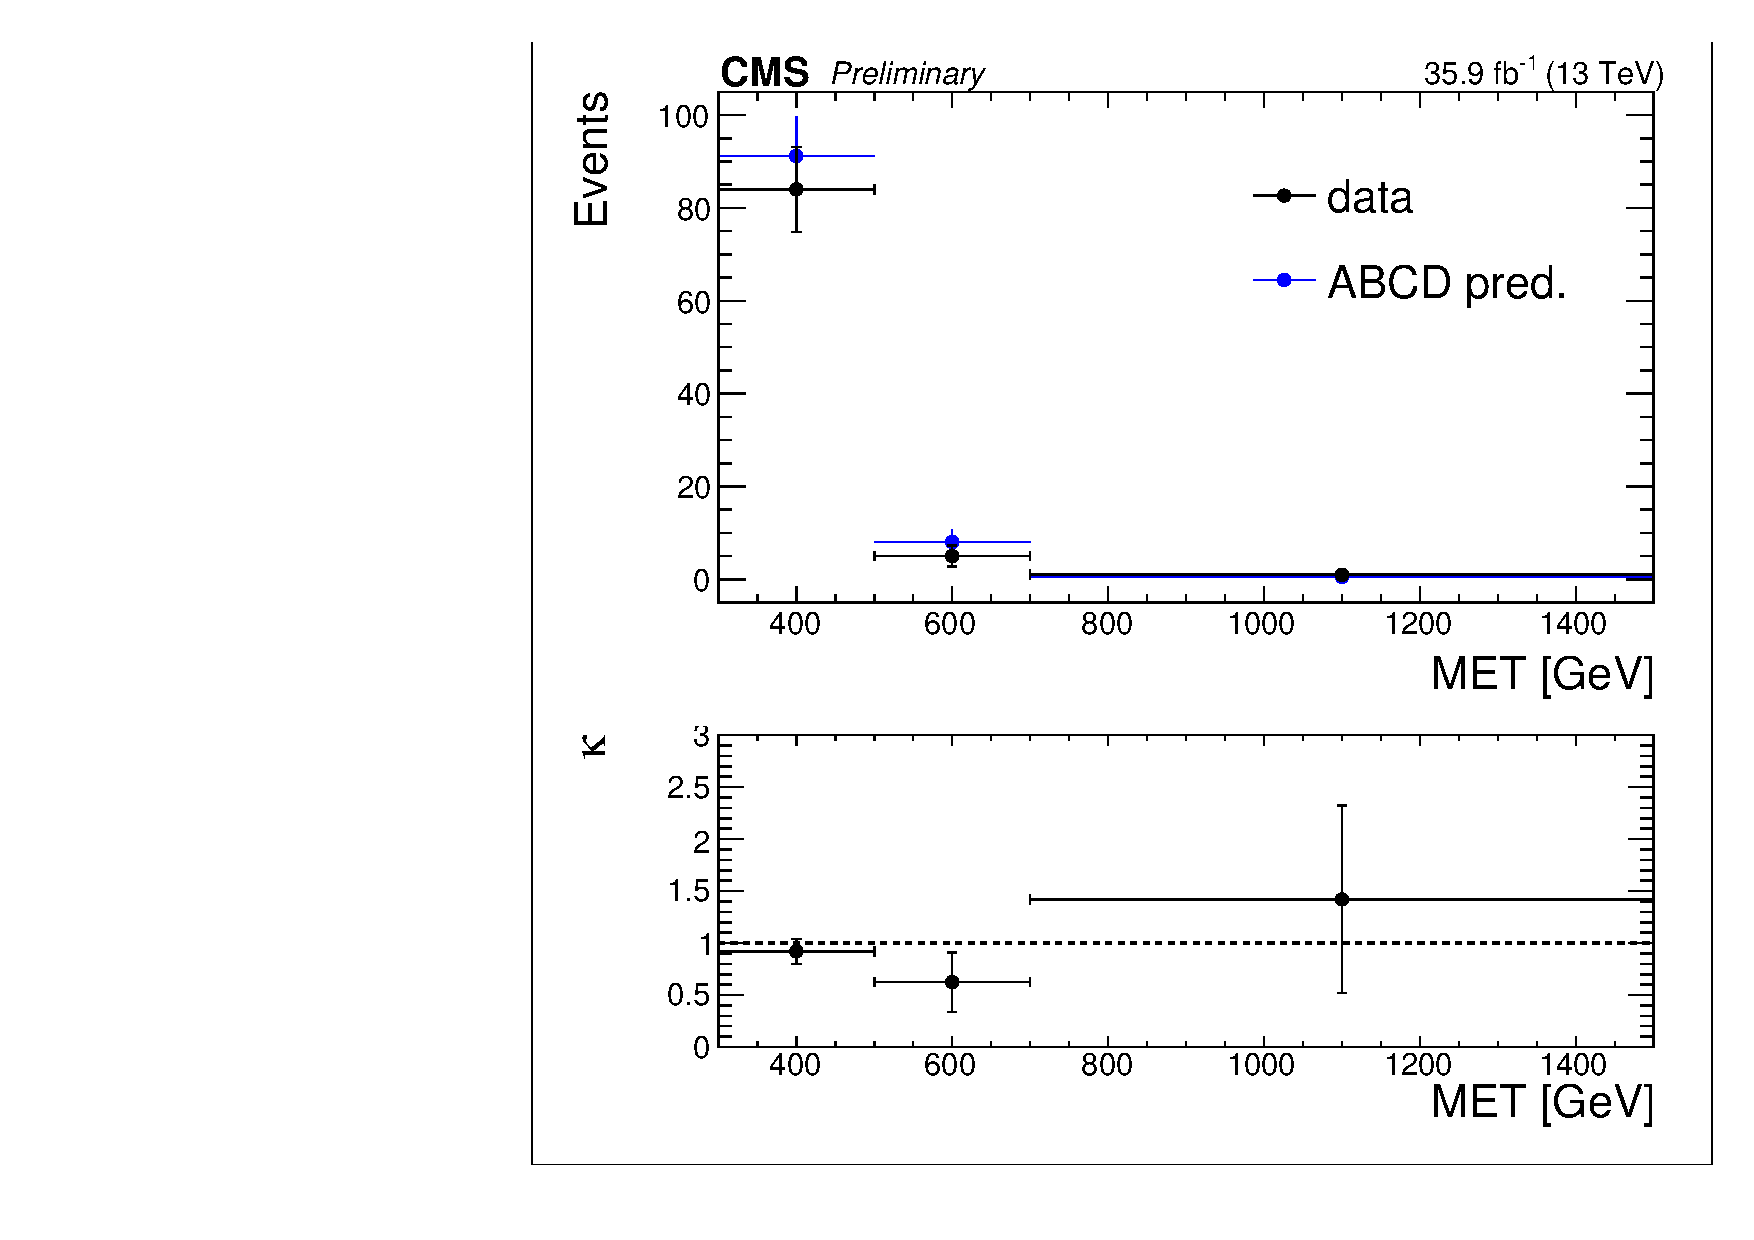
\includegraphics[trim={5px 5px 5px 5px},clip,width=0.95\textwidth]{figs/dataClosure_single-tagSR_lowDphi.pdf} 
\caption{low-$\Delta\phi$ A$_{1}$}
\end{subfigure}
\begin{subfigure}[b]{0.42\textwidth}
\centering
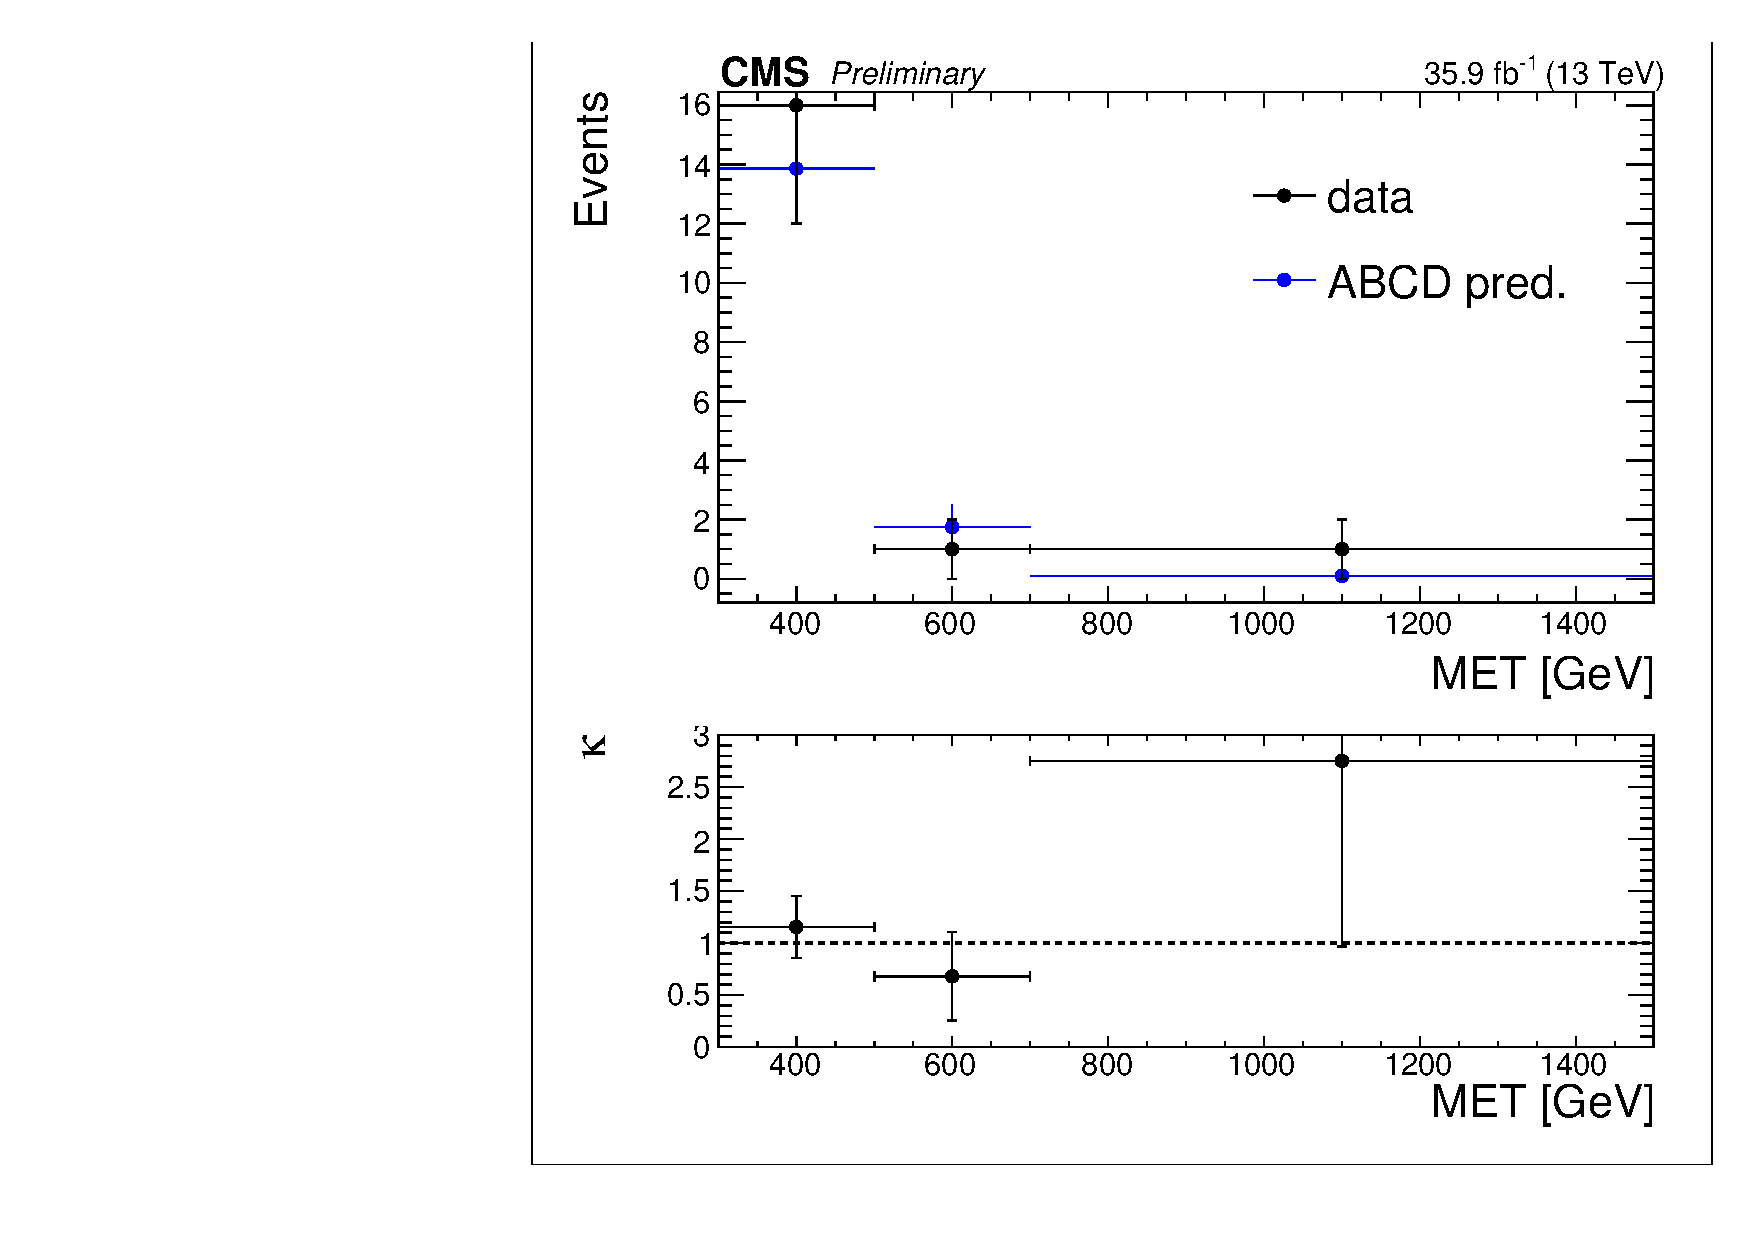
\includegraphics[trim={5px 5px 5px 5px},clip,width=0.95\textwidth]{figs/dataClosure_double-tagSR_lowDphi.pdf} 
\caption{low-$\Delta\phi$ A$_{2}$}
\end{subfigure}
\caption{Comparisons of the predicted and observed yields within the data control regions.}
\label{fig:closure}
\end{figure}

\subsection{$\kappa$ as a Correction to the Estimation}
\label{sec:kappa}

A correction factor $\kappa$ is applied to the prediction to account for the under-prediction of the background estimation procedure as observed in Figure~\ref{fig:MCclosure}. $\kappa$ is obtained by dividing the yields for the signal region by that predicted:

\begin{equation}
\kappa  \equiv A^{MC} \,/  \ \left(B \cdot \frac{C} {D} \ \right)^{MC}
\label{eq:kappa}
\end{equation}

There are 2x3=6 values of $\kappa$, one for each signal bin. $\kappa=1$ represents the case of a perfect prediction. The corrections are then applied as follows:

\begin{equation}
A_{1, 2}^{\mathrm{predicted}} = \kappa \cdot \left(B_{1, 2} \cdot \ \frac{C}{D}\right)^{\textrm{observed}}
\end{equation}

These values of $\kappa$ are those which we have already seen in Figure~\ref{fig:MCclosure}.

The value of $\kappa$ is dependent on the yields of each analysis bin and is therefore sensitive to the accuracy of the modeling of  in each of the 18 analysis bins. To improve the determination of $\kappa$, scale factors are derived using the data control regions to correct the normalization of  in each of these bins. Different scale factors are assigned separately to the Z-invisible, lost-lepton, and QCD background  samples. Rare processes (e.g. diboson) are taken directly from MC

First consider how the yield N predicted by  in an arbitrary bin (of 18) is the sum of the yields in the different  datasets ($t\bar{t}$ and $W\rightarrow\ell\nu$ are grouped as they together represent the lost-lepton background):

\begin{equation}
N^{MC} = N_{Z\rightarrow\nu\bar{\nu}}^{MC} + N_{t\bar{t},\,W\rightarrow\ell\nu}^{MC} + N_{QCD}^{MC} + N_{rare}
\end{equation}

Scale factors are defined for this bin using the corresponding control regions in data and forming the ratio of events in simulation to that observed. They are then applied as follows:

\begin{equation}
N_{corrected}^{MC} = \left(\frac{N_{single-\gamma}^{data}}{N_{single-\gamma}^{MC}}\right) \cdot N_{Z\rightarrow\nu\bar{\nu}}^{MC} + \left(\frac{N^{data}_{single-\ell}}{N^{MC}_{single-\ell}}\right) \cdot N^{MC}_{t\bar{t},\,W\rightarrow\ell\nu} + \left(\frac{N^{data}_{low-\Delta\phi}}{N^{MC}_{low-\Delta\phi}}\right) \cdot N_{QCD}^{MC} + N_{rare}
\end{equation}

The \ptmiss distribution within the control regions is shown for both data and  in Figures~\ref{fig:closurephoton},~\ref{fig:closuresinglelep},~\ref{fig:closurelowdphi} for the single photon, single lepton, and low-$\Delta\phi$ control regions, respectively. The ratio in the bottom panel of each plot represents the scale factor for that \ptmiss bin. The dotted horizontal line shows the average scale factor inclusive in \ptmiss. The scale factors for the single-photon and low-$\Delta\phi$ control regions show no \ptmiss dependence and are determined integrated over \ptmiss$>300\,\textrm{GeV}$. The values of the scale factors are summarized in Table~\ref{tab:ScaleFactorVR}. The Single-lepton region, shown in Figure~\ref{fig:closuresinglelep}, does show \ptmiss dependence and are summarized in Tables~\ref{tab:ScaleFactorVR}~and~\ref{tab:ScaleFactorMET}.  In order to improve statistics for the single-lepton region, the low-$\Delta\phi$ requirement has been removed.

\begin{figure}
 \centering
 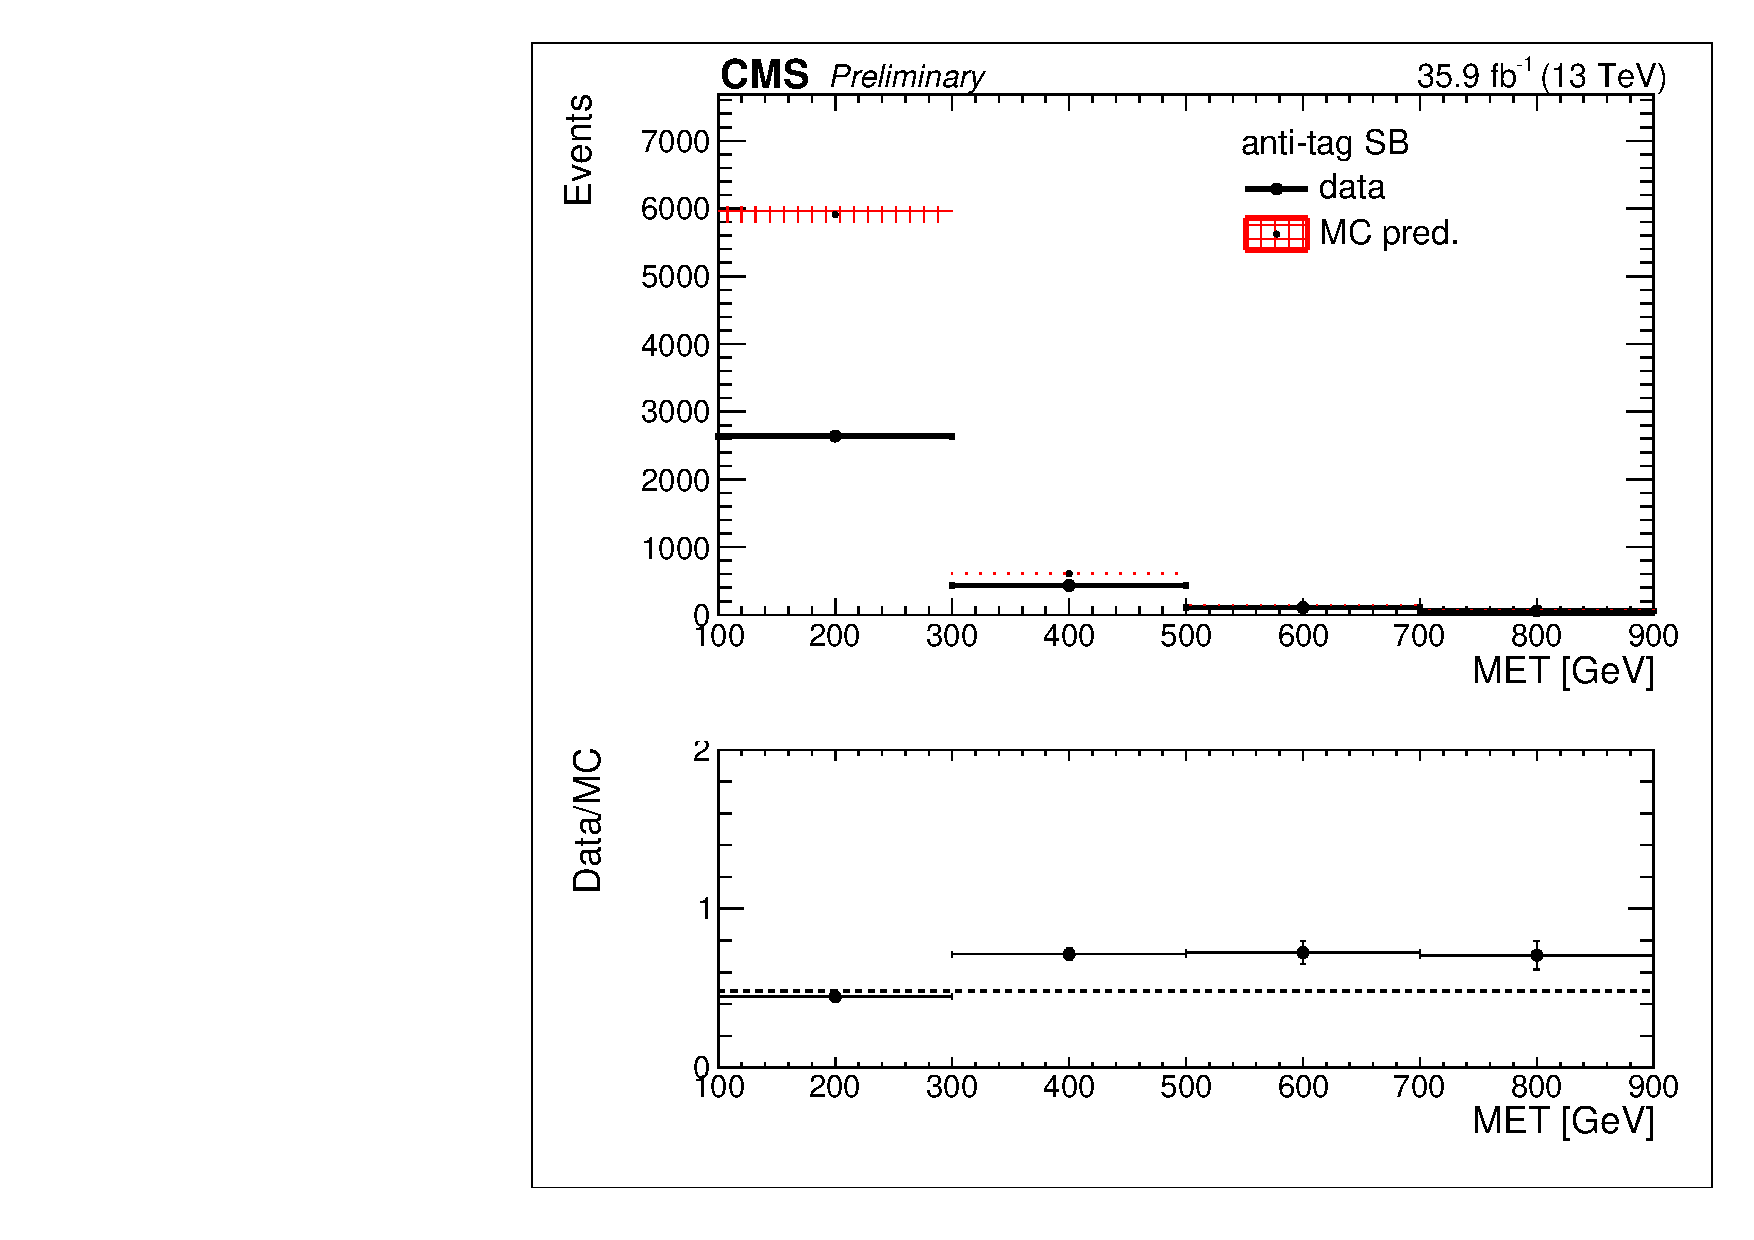
\includegraphics[trim={5px 5px 5px 5px},clip,width=0.425\linewidth]{figs/ABCDscaleFactors_MET_antitagSB_photon.pdf}
 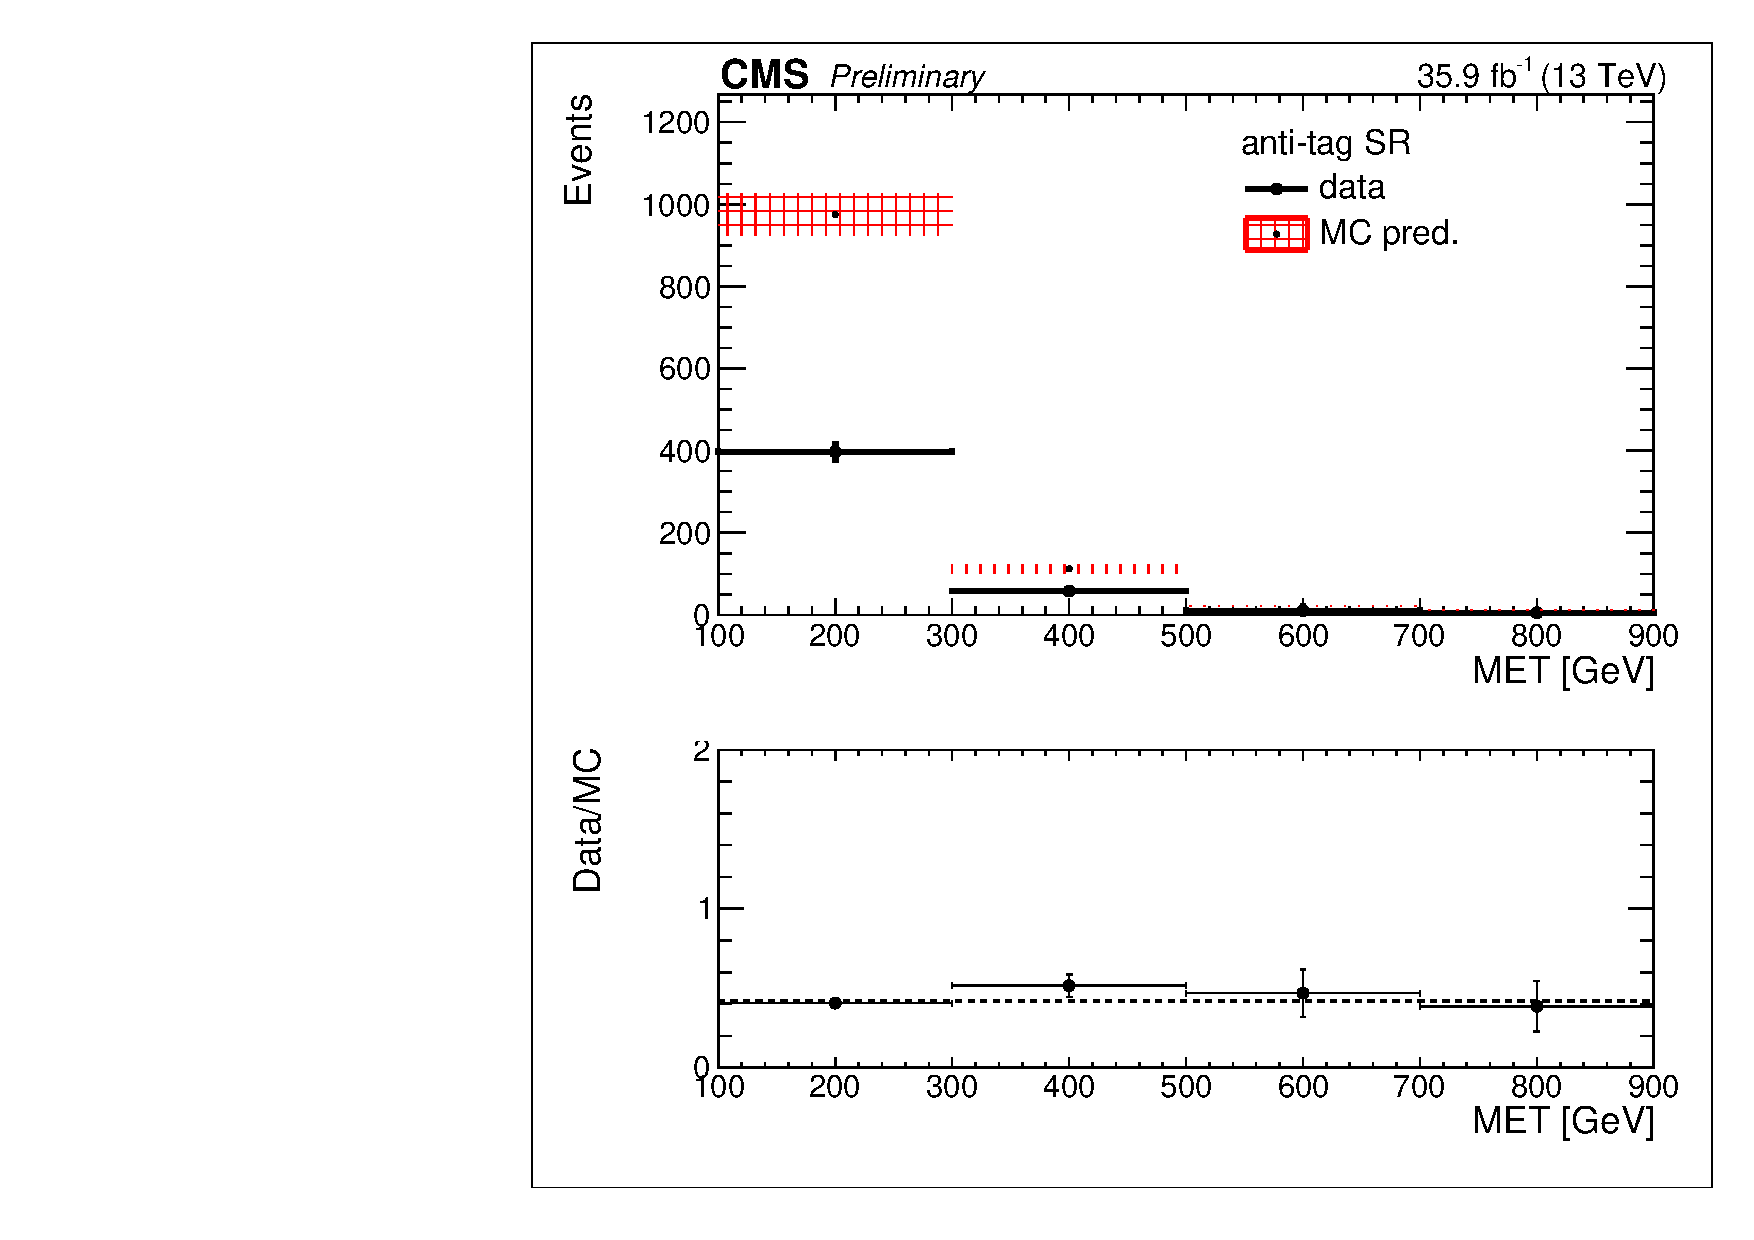
\includegraphics[trim={5px 5px 5px 5px},clip,width=0.425\linewidth]{figs/ABCDscaleFactors_MET_antitagSR_photon.pdf}\\
 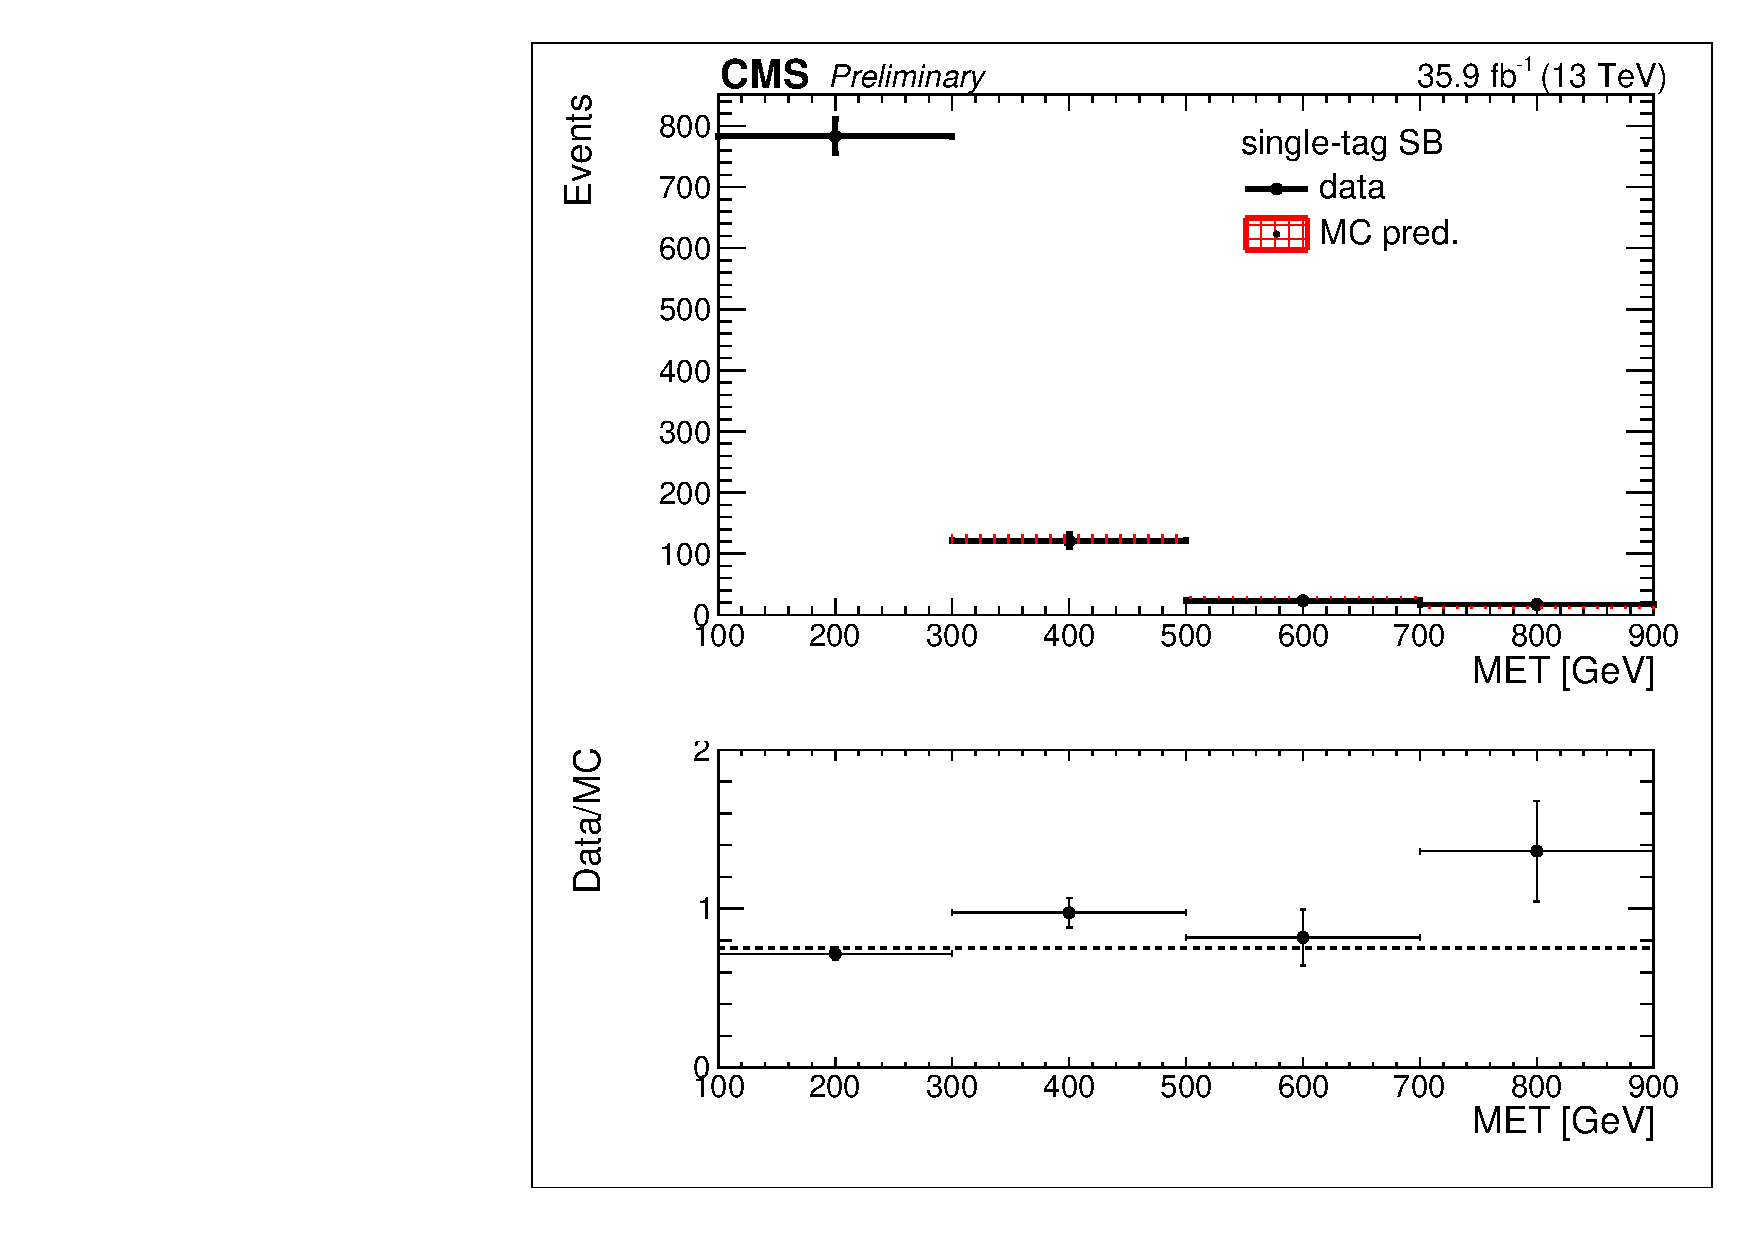
\includegraphics[trim={5px 5px 5px 5px},clip,width=0.425\linewidth]{figs/ABCDscaleFactors_MET_single-tagSB_photon.pdf}
 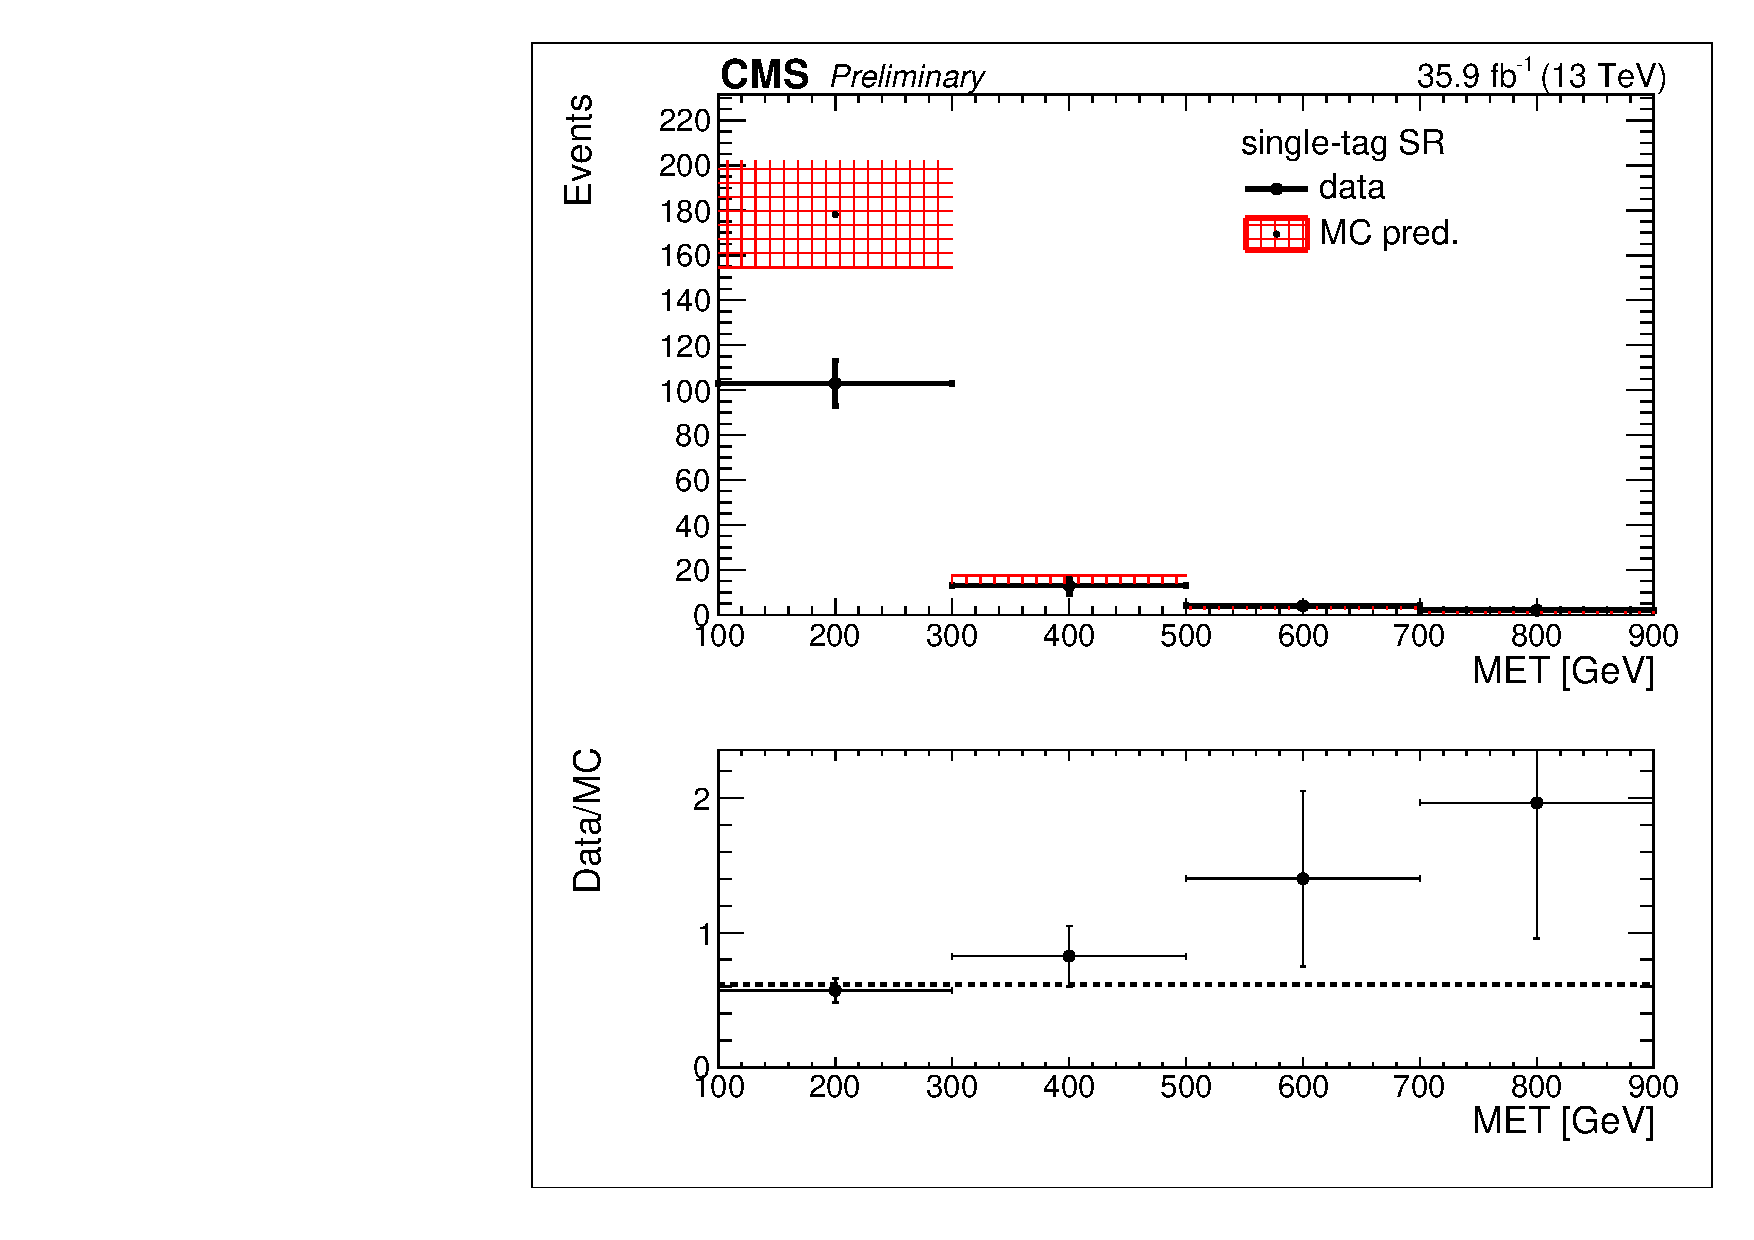
\includegraphics[trim={5px 5px 5px 5px},clip,width=0.425\linewidth]{figs/ABCDscaleFactors_MET_single-tagSR_photon.pdf}\\
 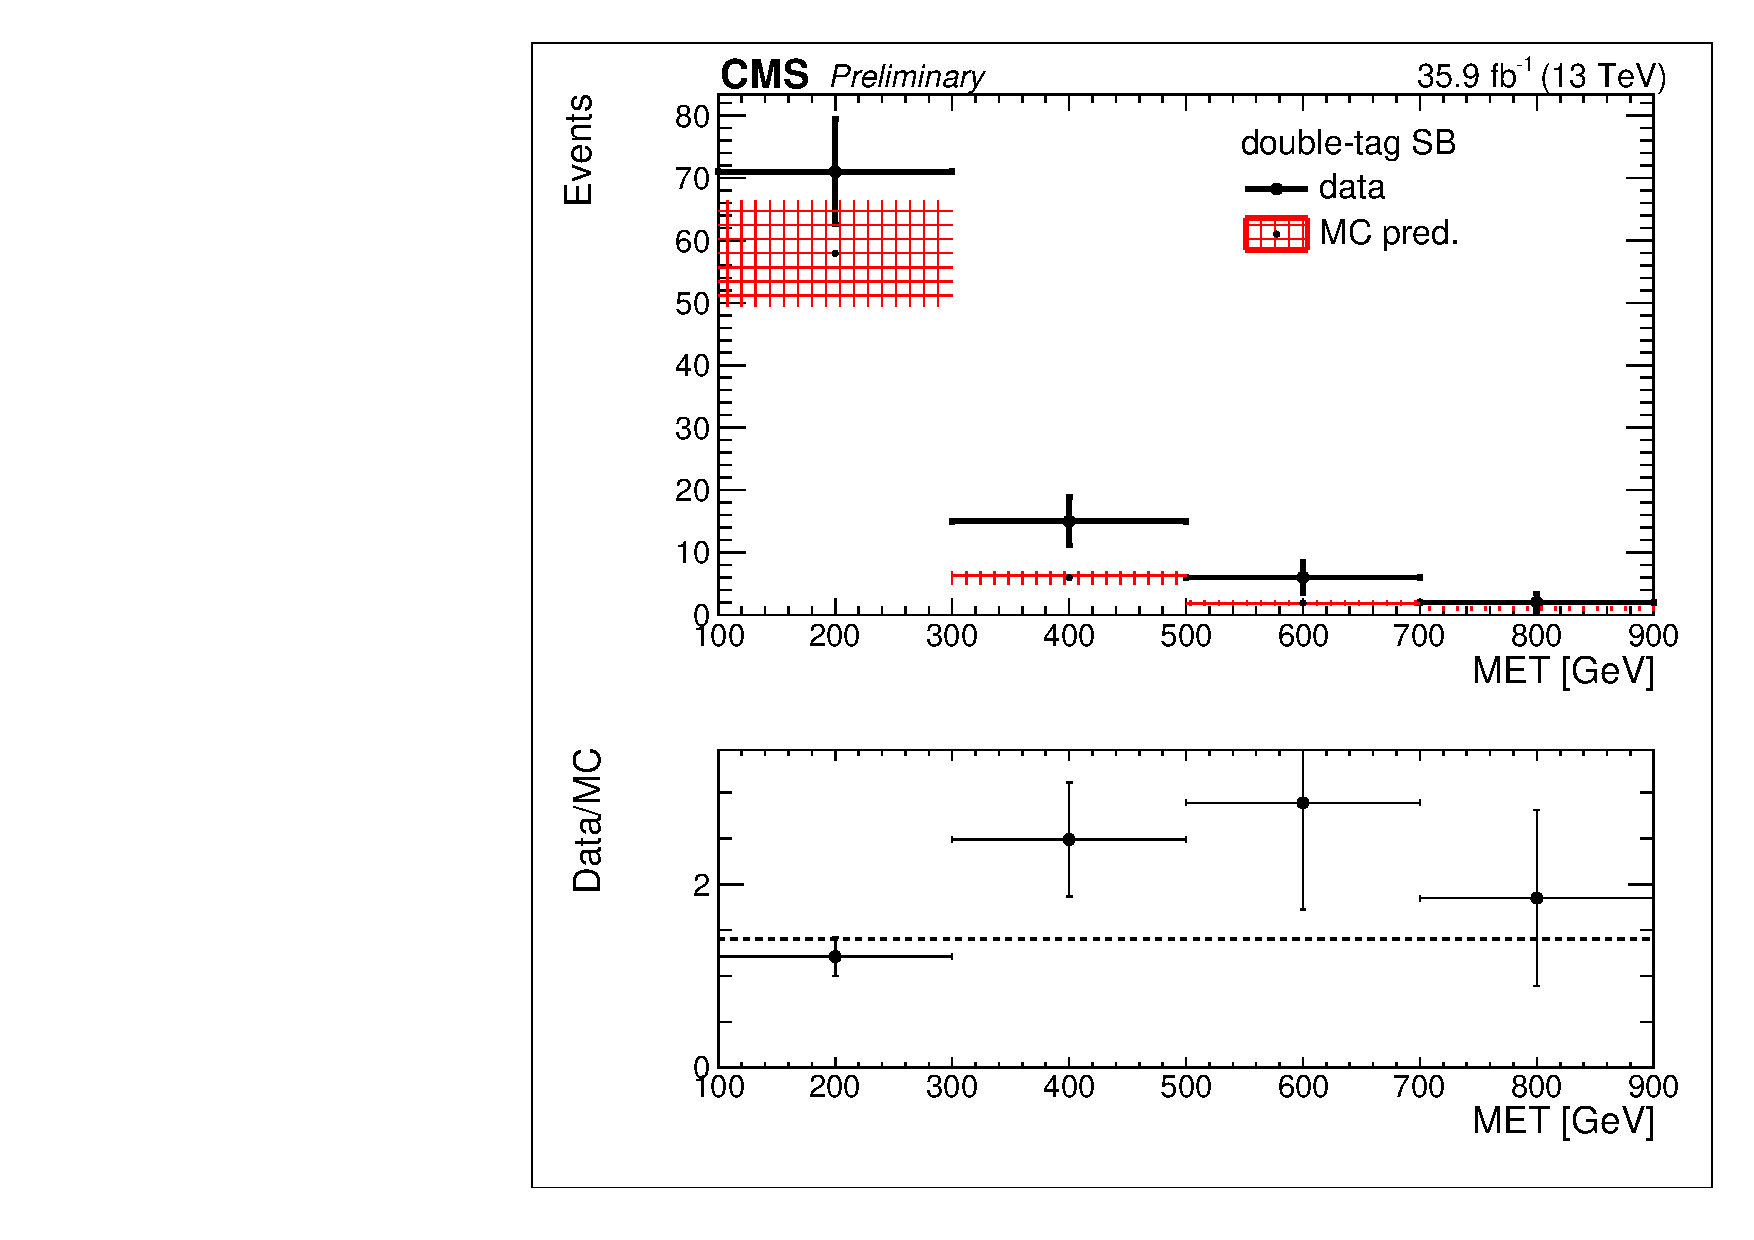
\includegraphics[trim={5px 5px 5px 5px},clip,width=0.425\linewidth]{figs/ABCDscaleFactors_MET_double-tagSB_photon.pdf}
 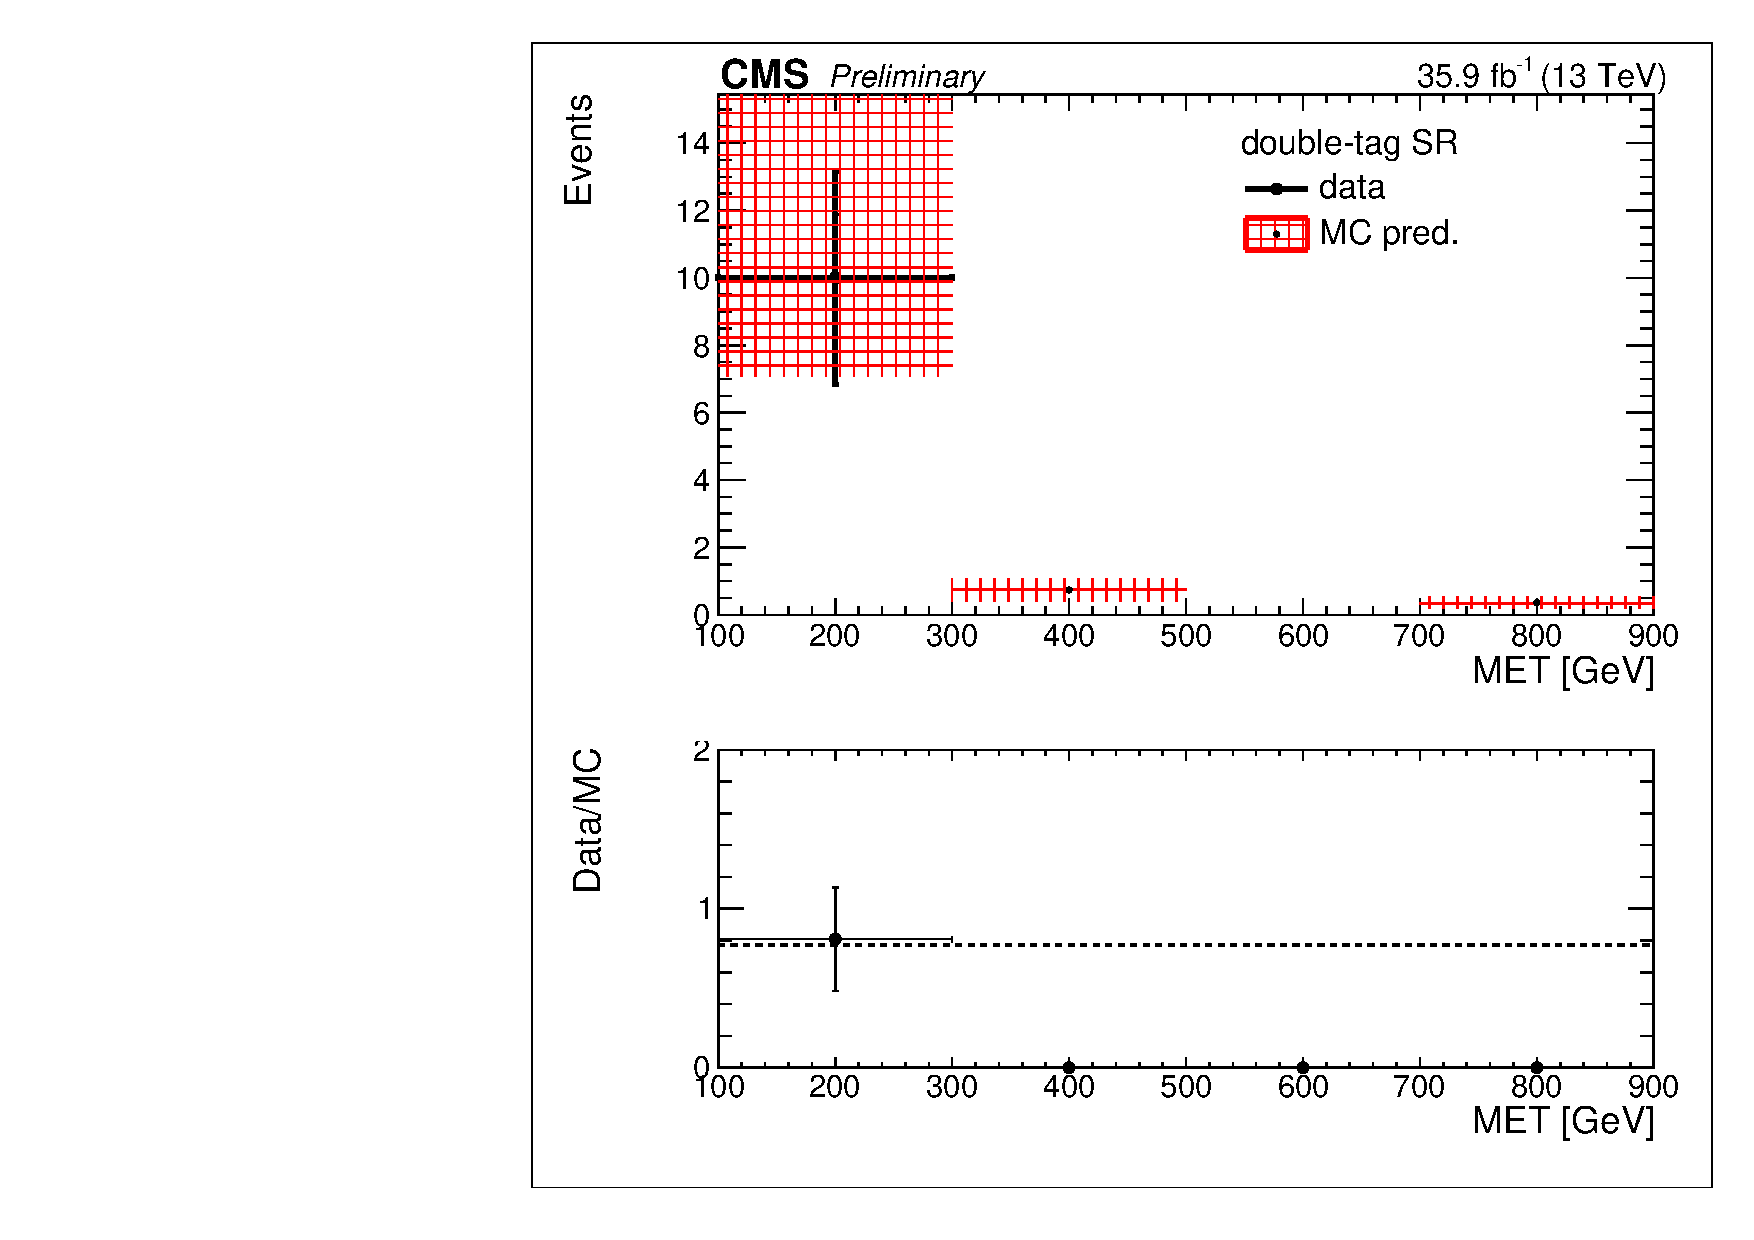
\includegraphics[trim={5px 5px 5px 5px},clip,width=0.425\linewidth]{figs/ABCDscaleFactors_MET_double-tagSR_photon.pdf}\\
 \caption
 [Signal and sideband yields in the single photon control region.]
 {Signal and sideband yields in the single photon control region. The hashed red band denotes the prediction from simulation; the solid black points denote the observed yields in data. The Data/ ratio in the lower panel of each plot represents the scale factor for that bin. }
\label{fig:closurephoton}
\end{figure}

\begin{figure}
\centering
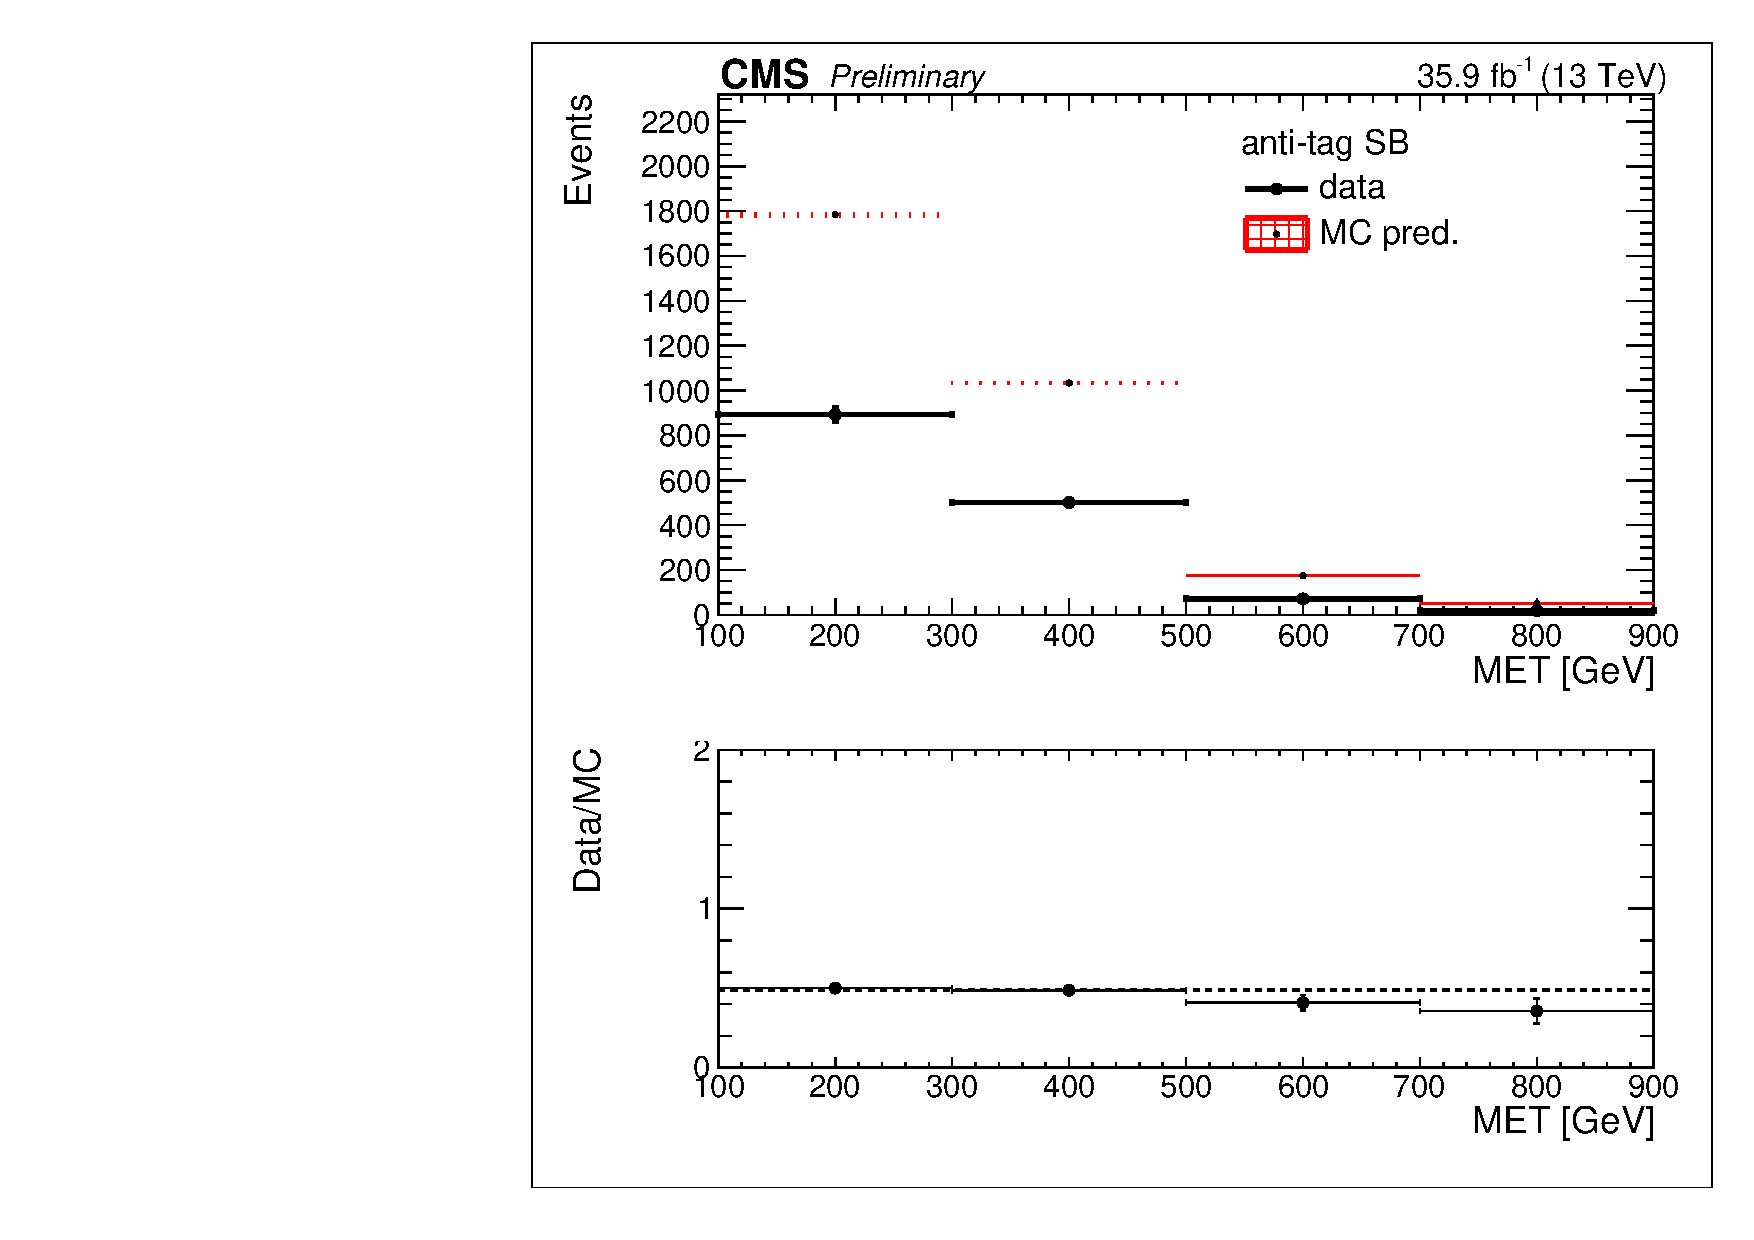
\includegraphics[trim={5px 5px 5px 5px},clip,width=0.425\linewidth]{figs/ABCDscaleFactors_MET_antitagSB_lowDeltaPhi_singleLep.pdf}
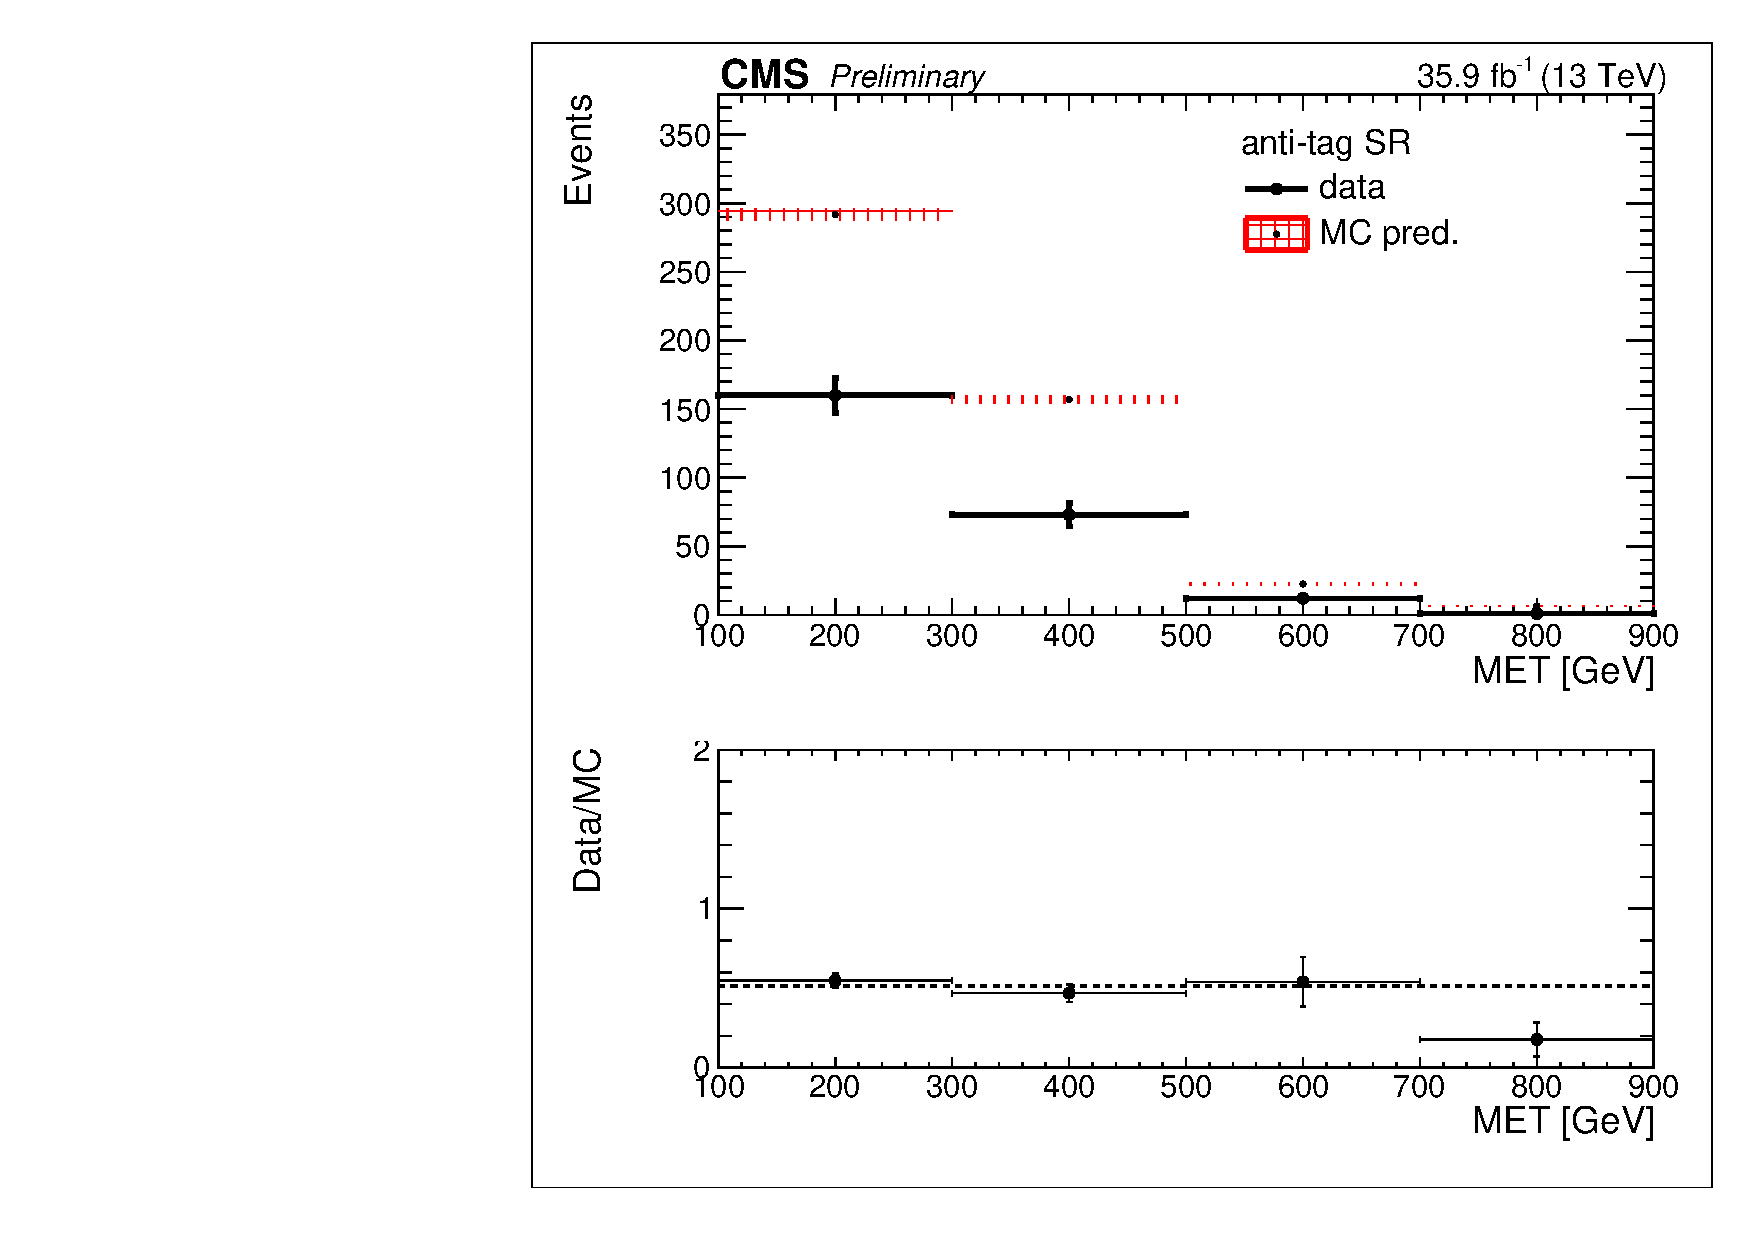
\includegraphics[trim={5px 5px 5px 5px},clip,width=0.425\linewidth]{figs/ABCDscaleFactors_MET_antitagSR_lowDeltaPhi_singleLep.pdf}\\
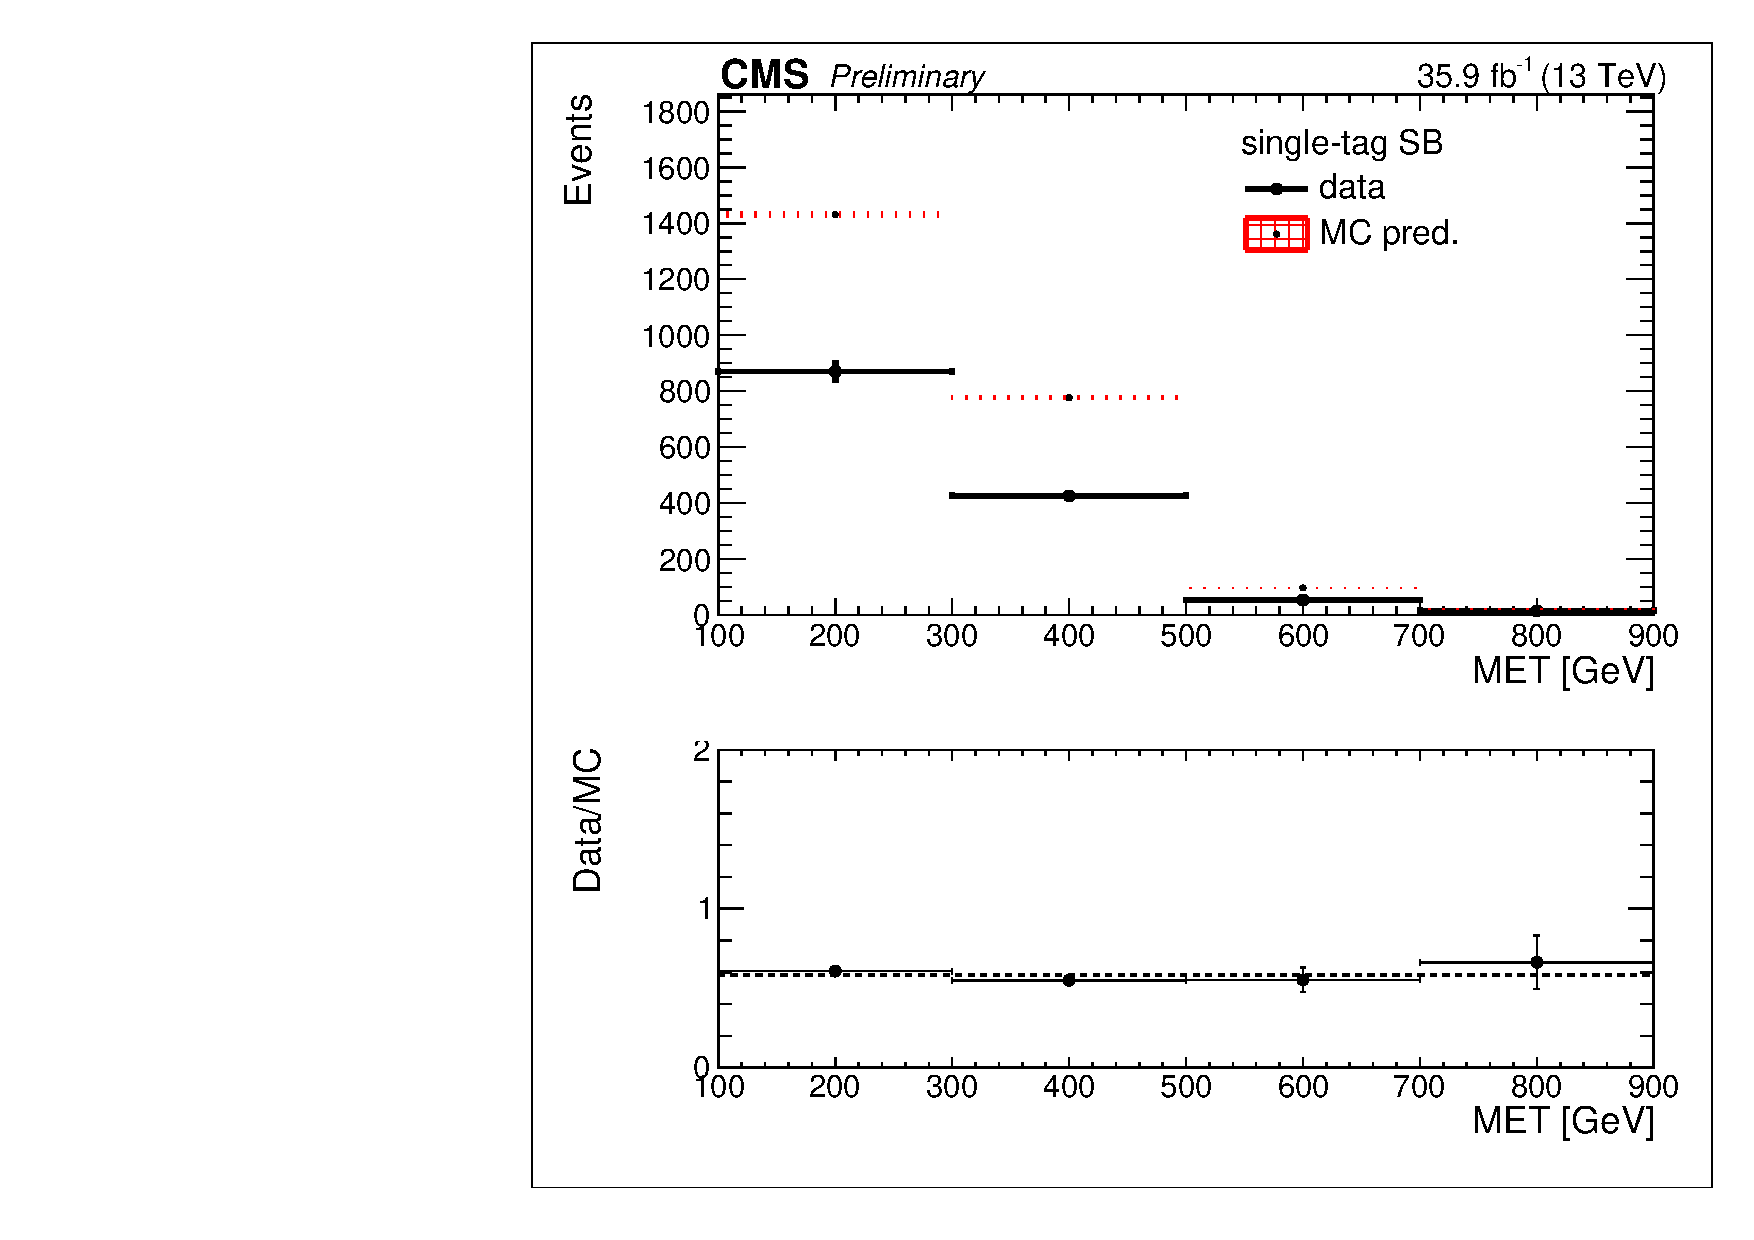
\includegraphics[trim={5px 5px 5px 5px},clip,width=0.425\linewidth]{figs/ABCDscaleFactors_MET_tagSB_lowDeltaPhi_singleLep.pdf}
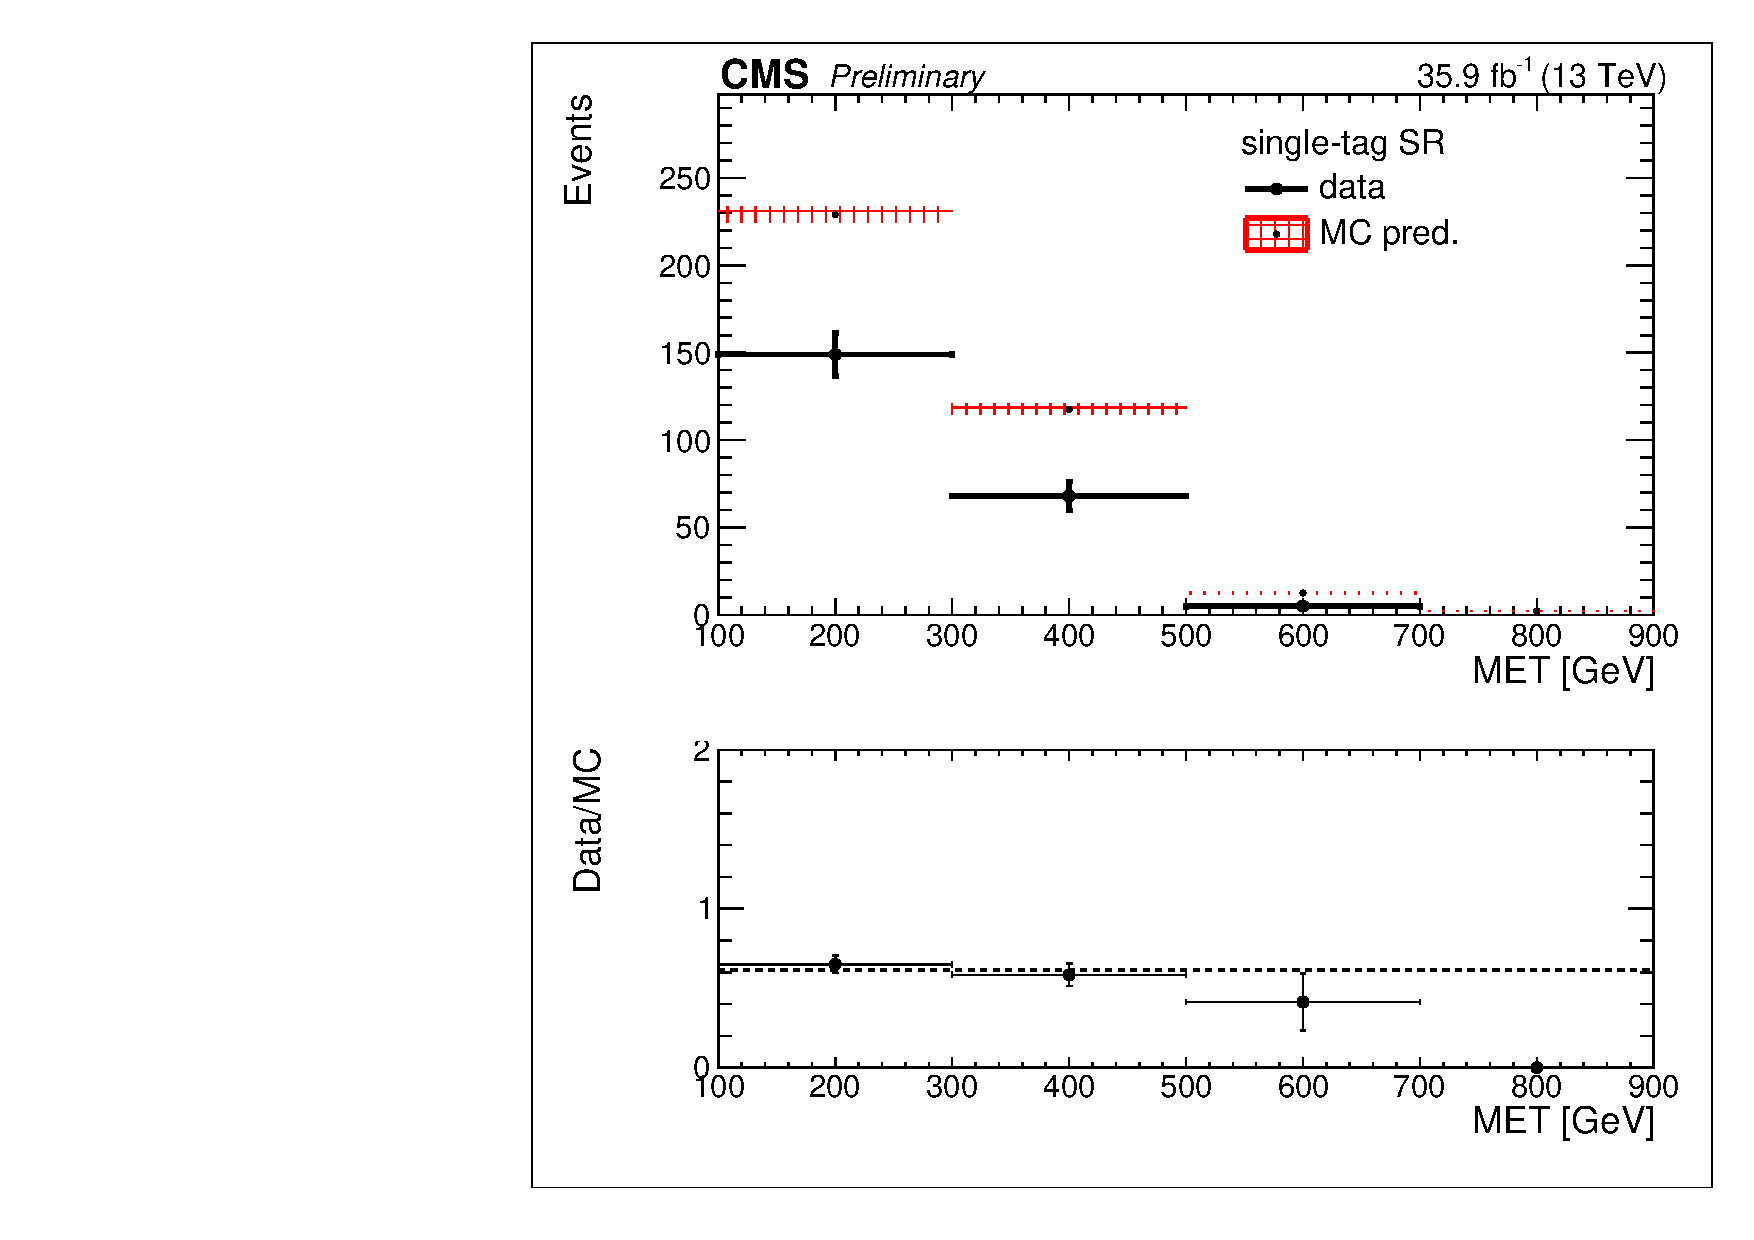
\includegraphics[trim={5px 5px 5px 5px},clip,width=0.425\linewidth]{figs/ABCDscaleFactors_MET_tagSR_lowDeltaPhi_singleLep.pdf}\\
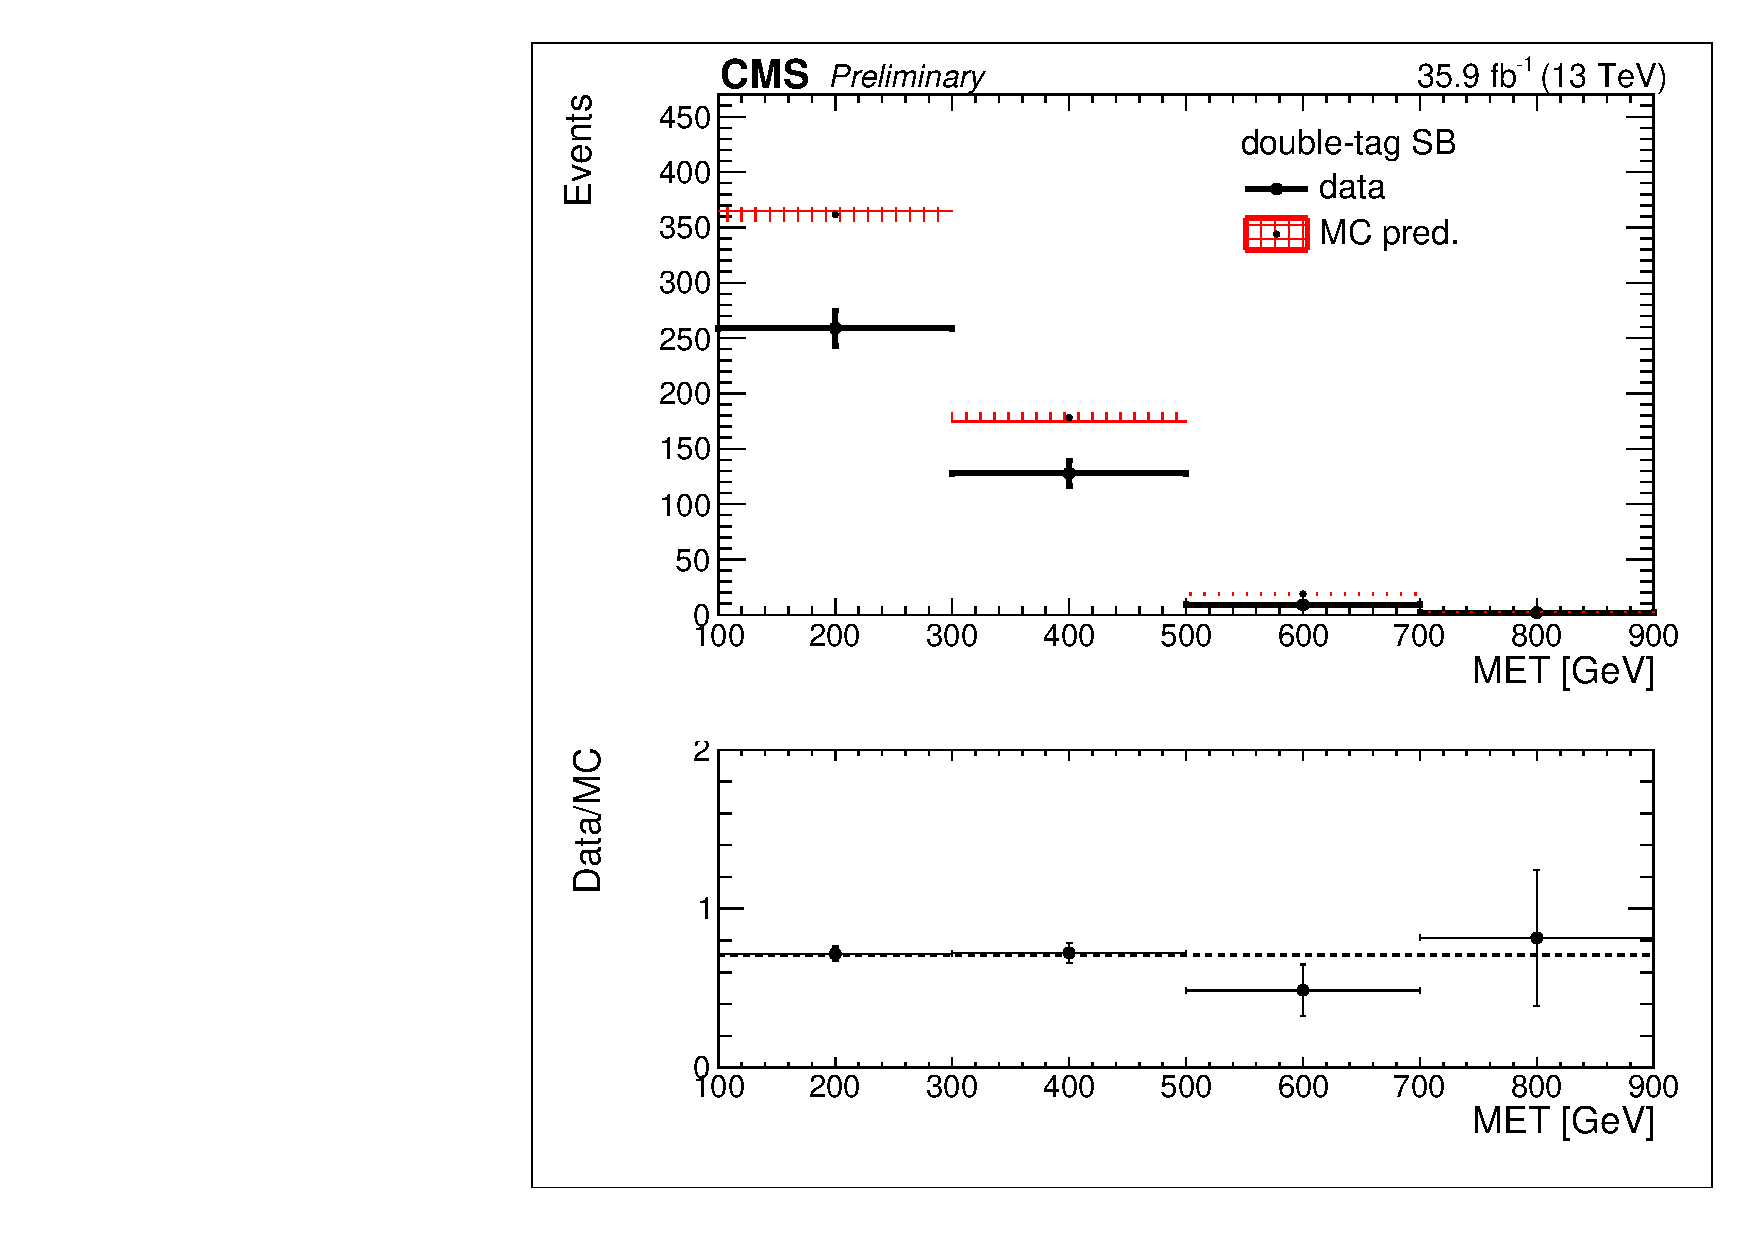
\includegraphics[trim={5px 5px 5px 5px},clip,width=0.425\linewidth]{figs/ABCDscaleFactors_MET_double-tagSB_lowDeltaPhi_singleLep.pdf}
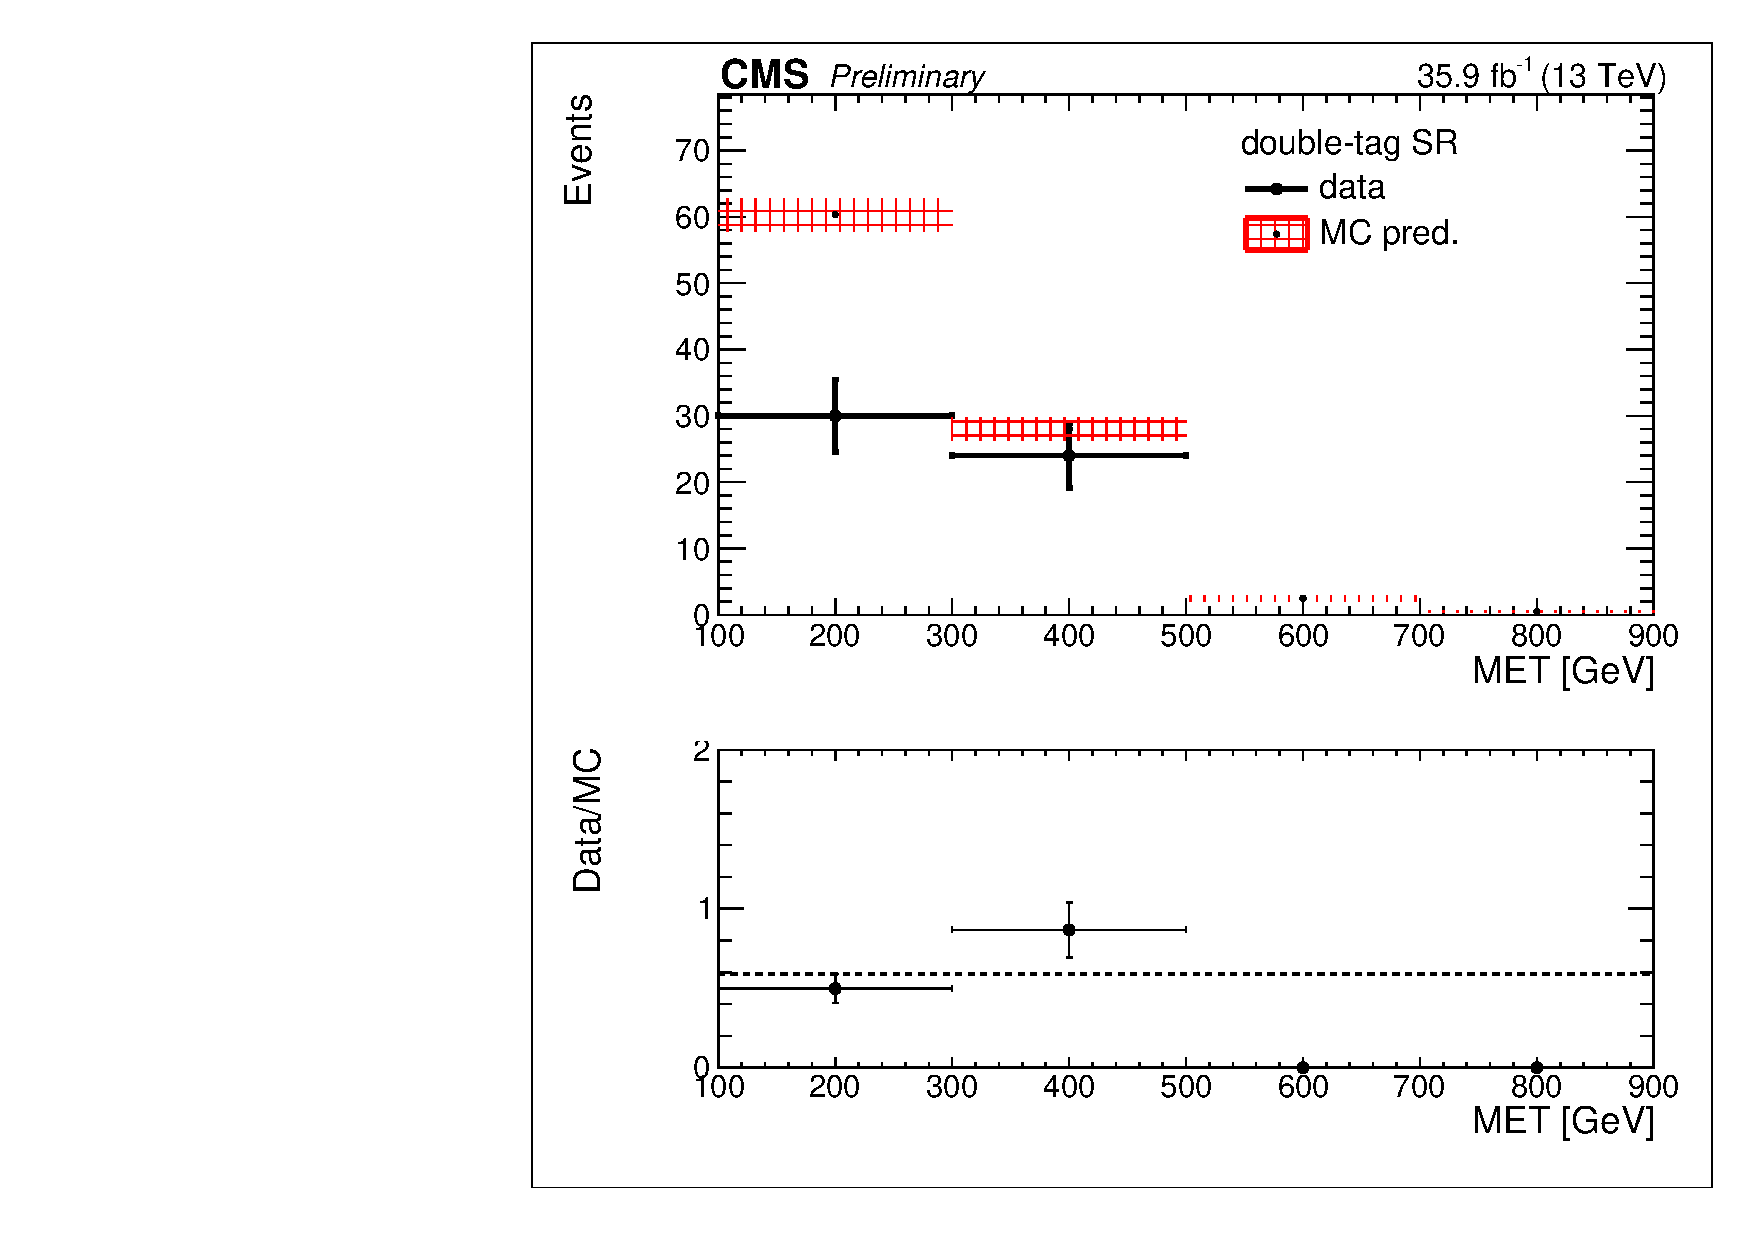
\includegraphics[trim={5px 5px 5px 5px},clip,width=0.425\linewidth]{figs/ABCDscaleFactors_MET_double-tagSR_lowDeltaPhi_singleLep.pdf}\\
\caption
[Signal and sideband yields in the single lepton control region.]
{Signal and sideband yields in the single lepton control region. The hashed red band denotes the prediction from simulation; the solid black points denote the observed yields in data. The Data/ ratio in the lower panel of each plot represents the scale factor for that bin. The low-$\Delta\phi$ requirement has been removed to improve statistics.}
\label{fig:closuresinglelep}
\end{figure}

\begin{figure}
 \centering
 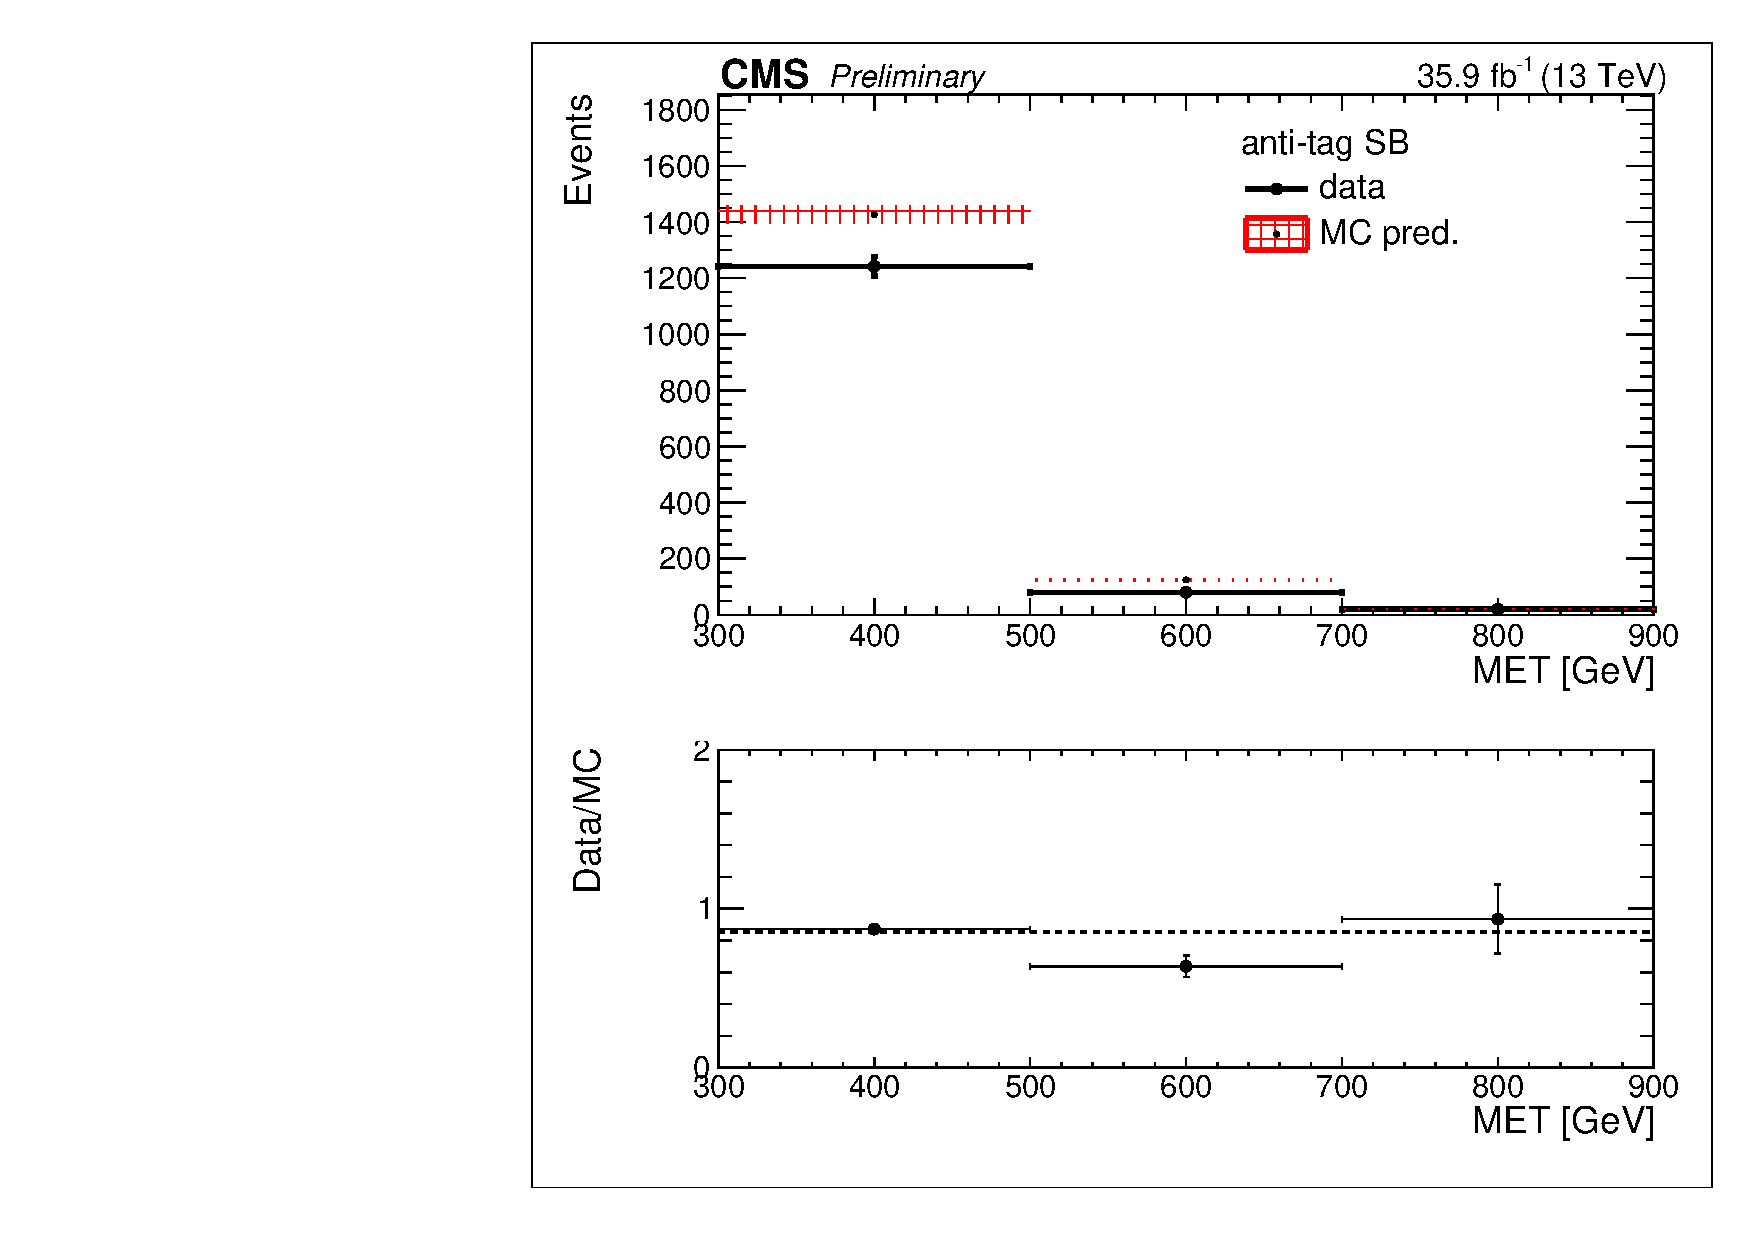
\includegraphics[trim={5px 5px 5px 5px},clip,width=0.425\linewidth]{figs/ABCDscaleFactors_MET_antitagSB_lowDphi.pdf}
 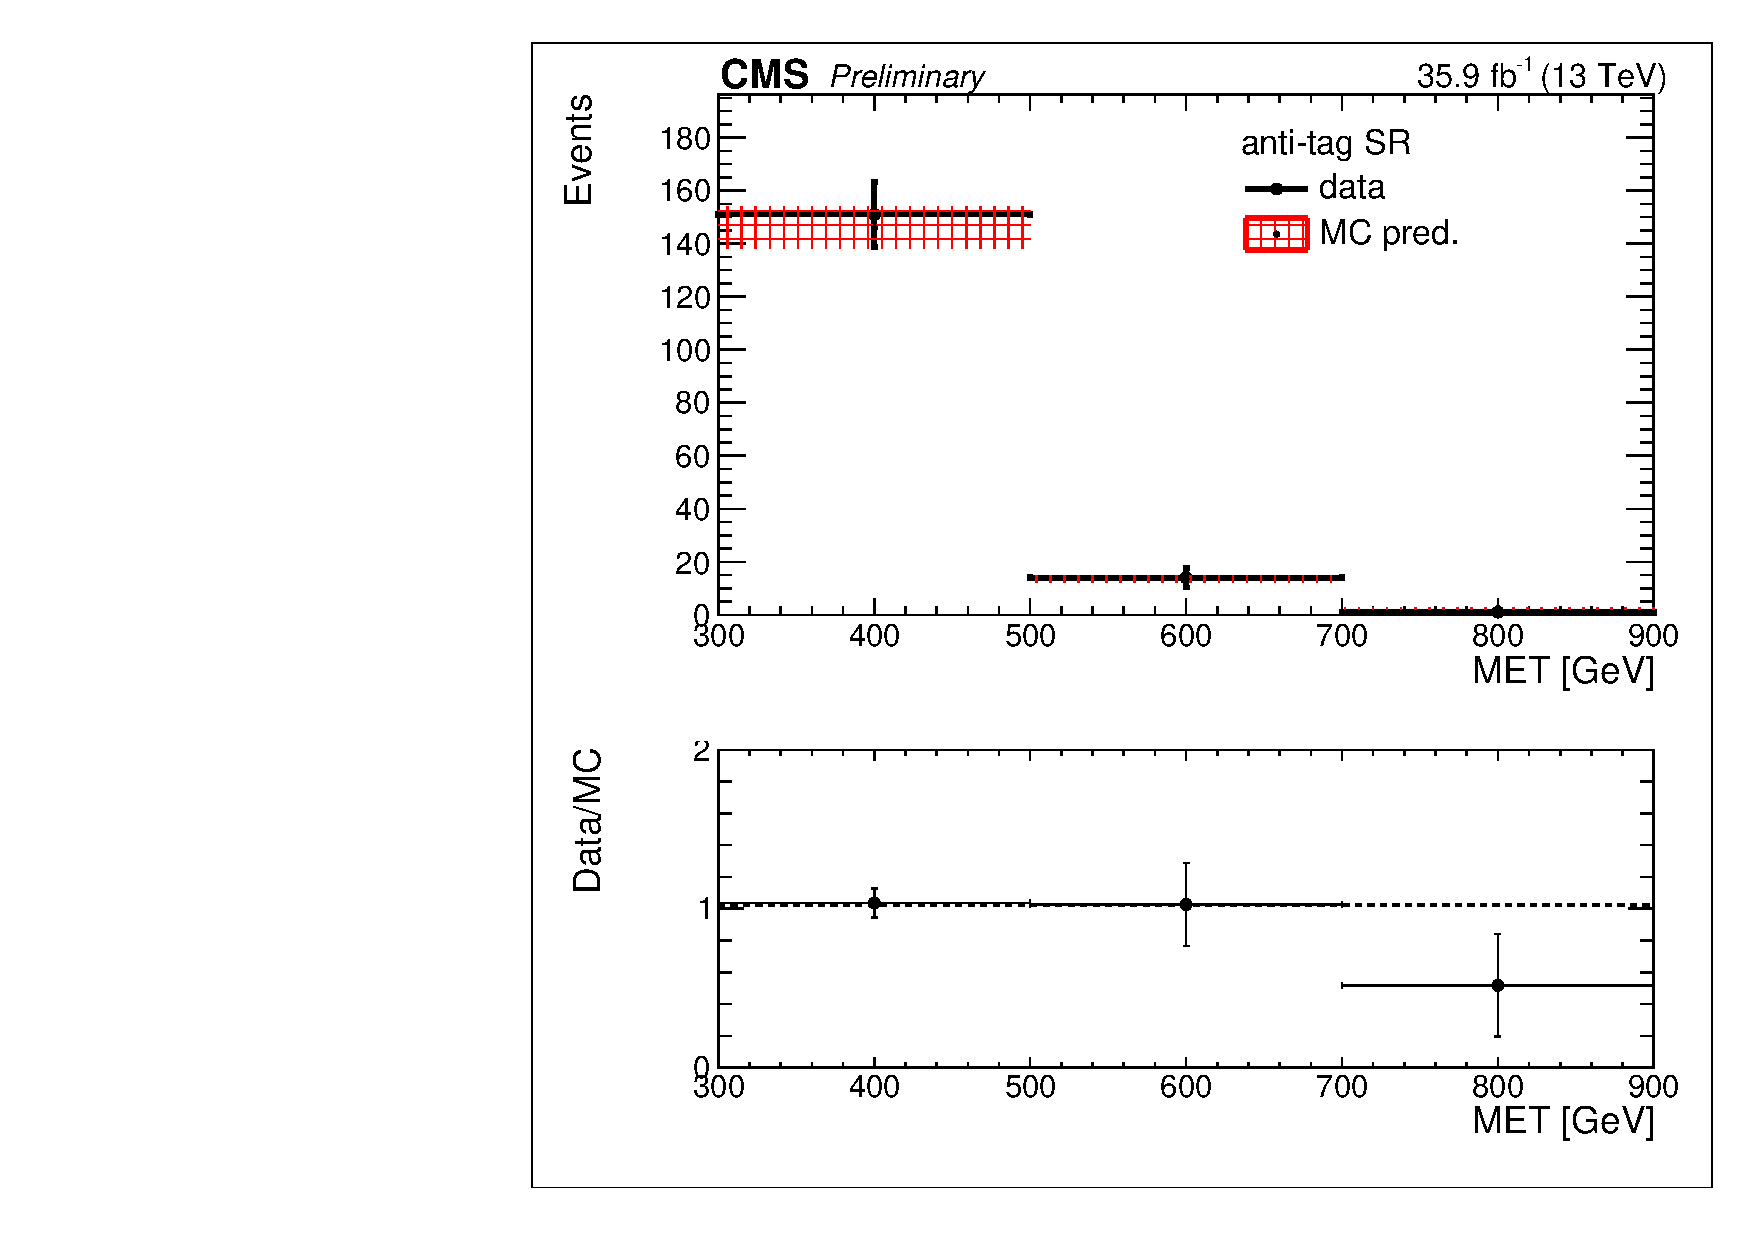
\includegraphics[trim={5px 5px 5px 5px},clip,width=0.425\linewidth]{figs/ABCDscaleFactors_MET_antitagSR_lowDphi.pdf}\\
 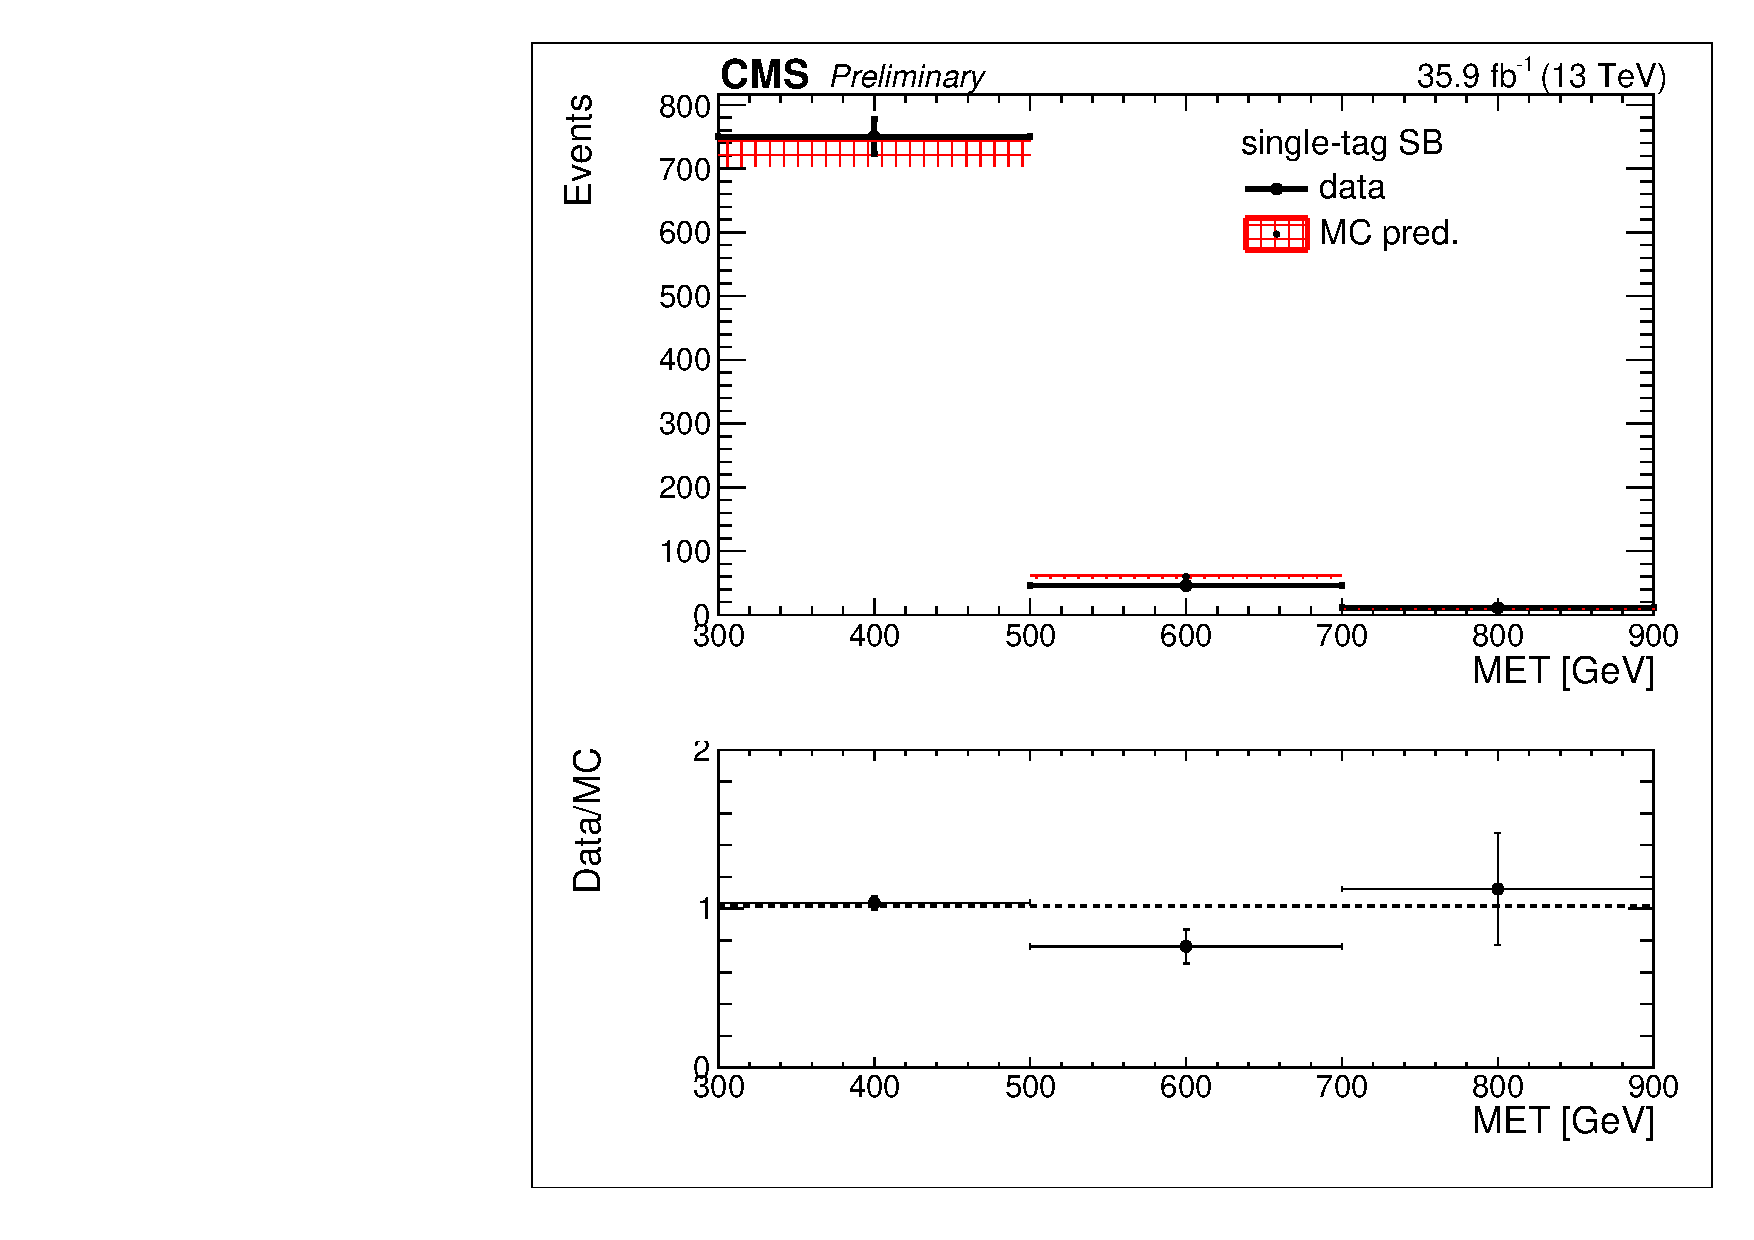
\includegraphics[trim={5px 5px 5px 5px},clip,width=0.425\linewidth]{figs/ABCDscaleFactors_MET_single-tagSB_lowDphi.pdf}
 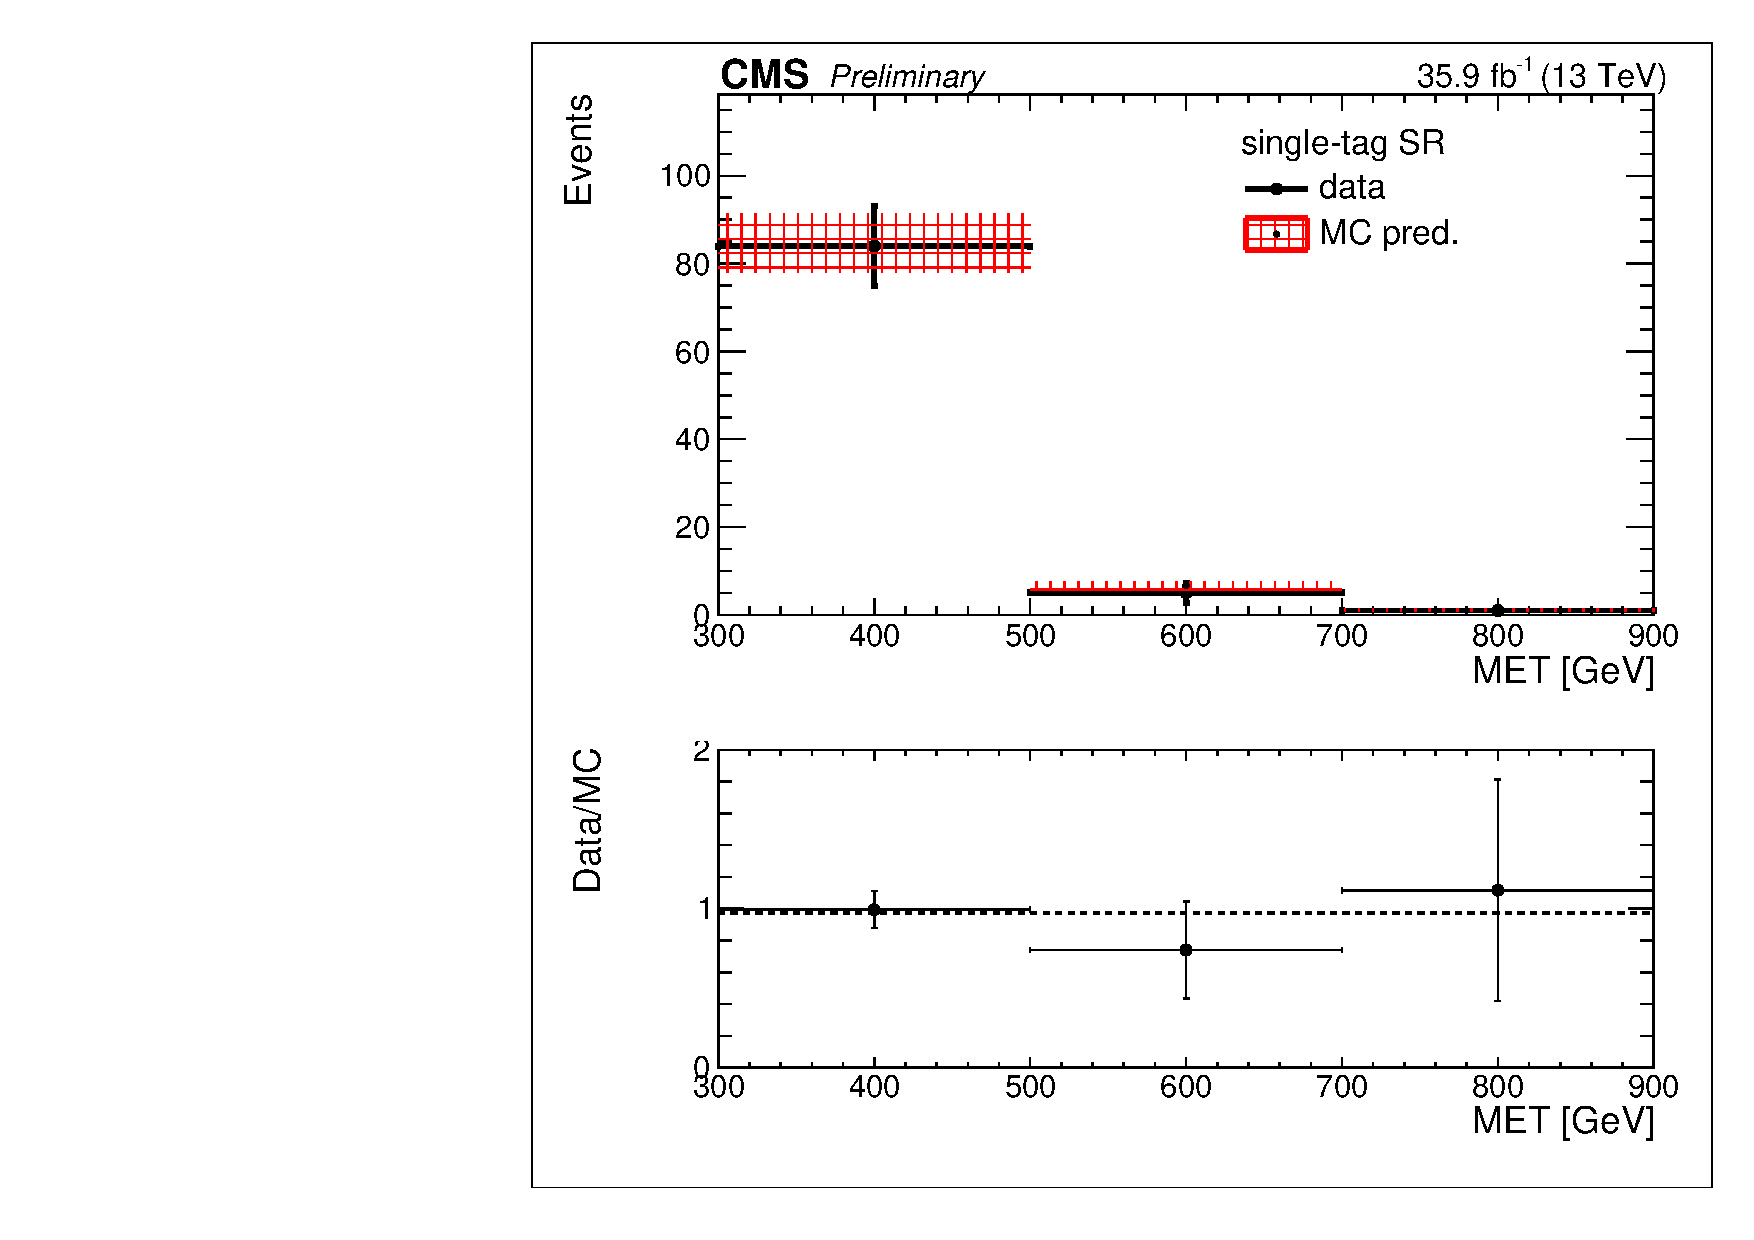
\includegraphics[trim={5px 5px 5px 5px},clip,width=0.425\linewidth]{figs/ABCDscaleFactors_MET_single-tagSR_lowDphi.pdf}\\
 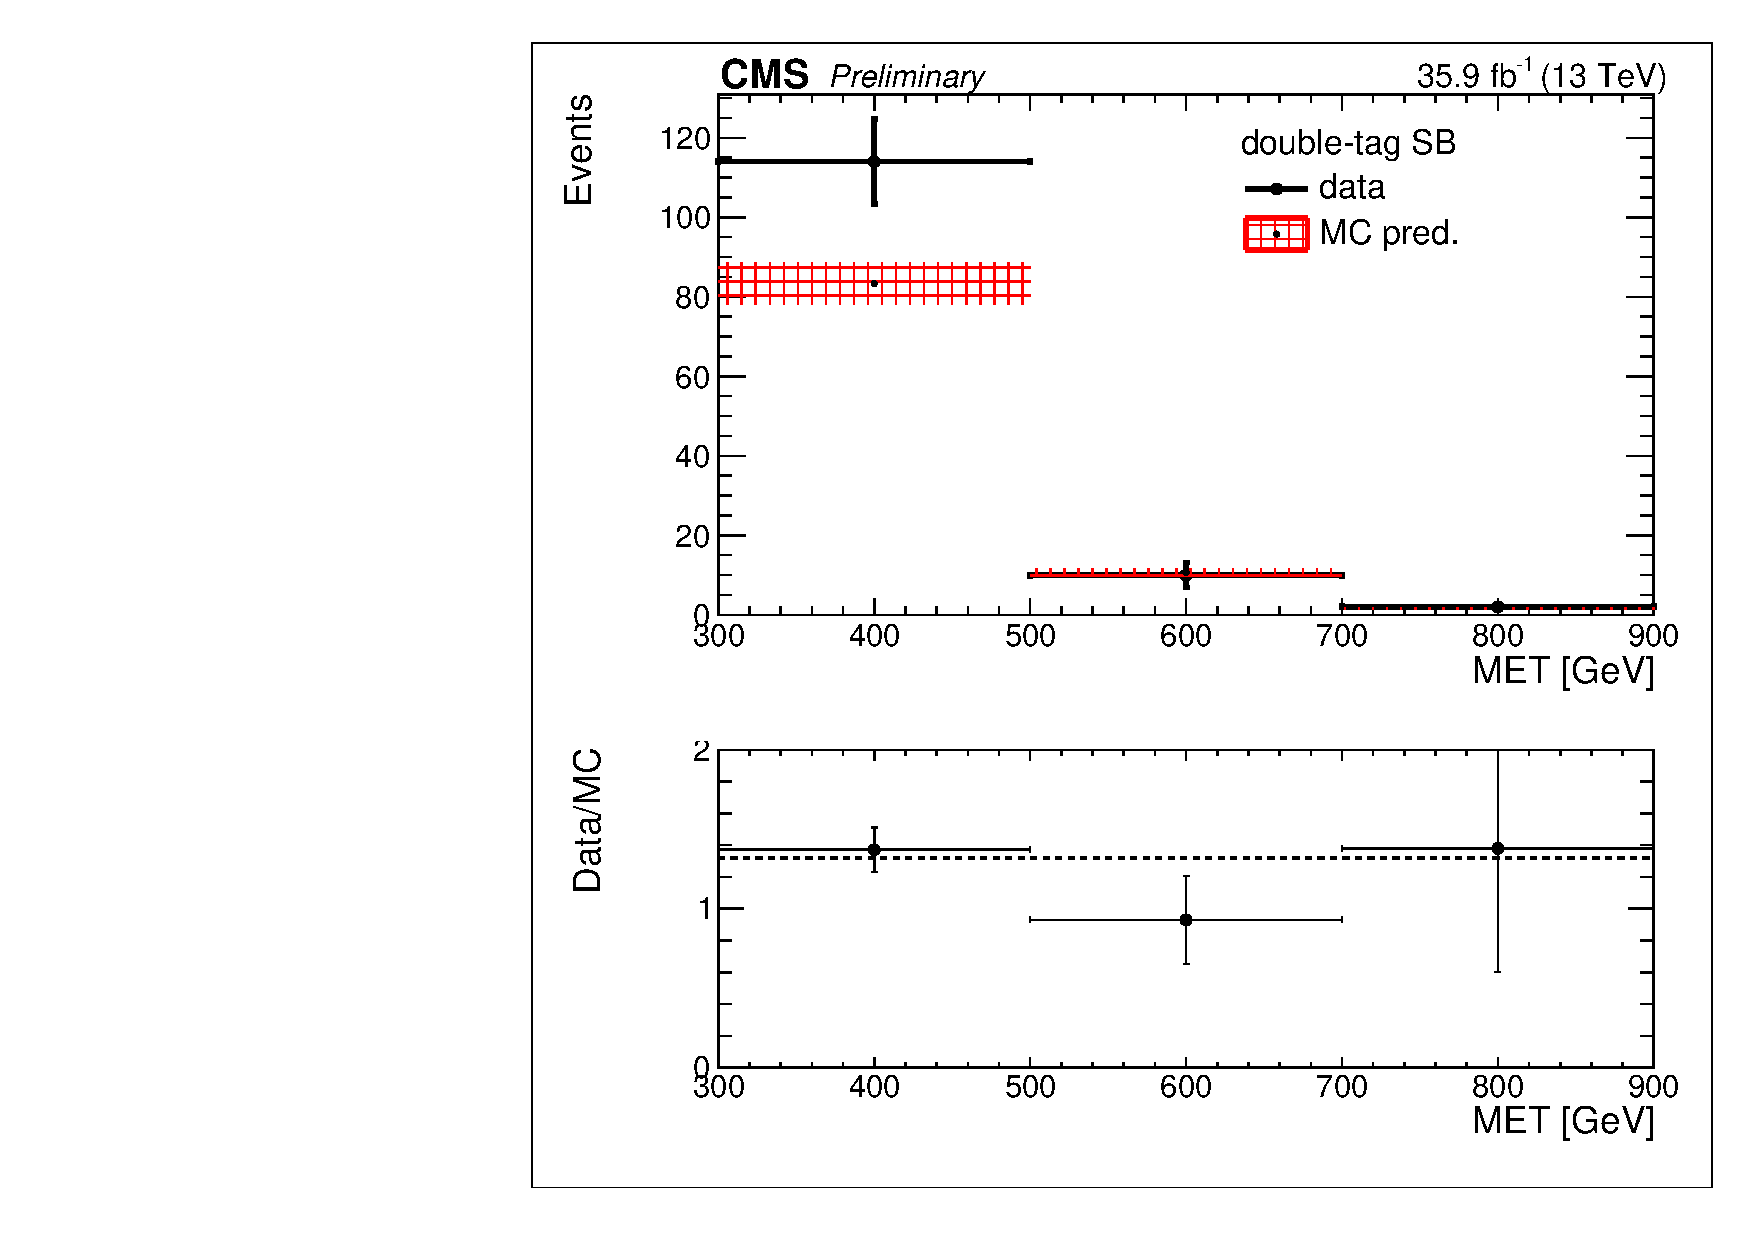
\includegraphics[trim={5px 5px 5px 5px},clip,width=0.425\linewidth]{figs/ABCDscaleFactors_MET_double-tagSB_lowDphi.pdf}
 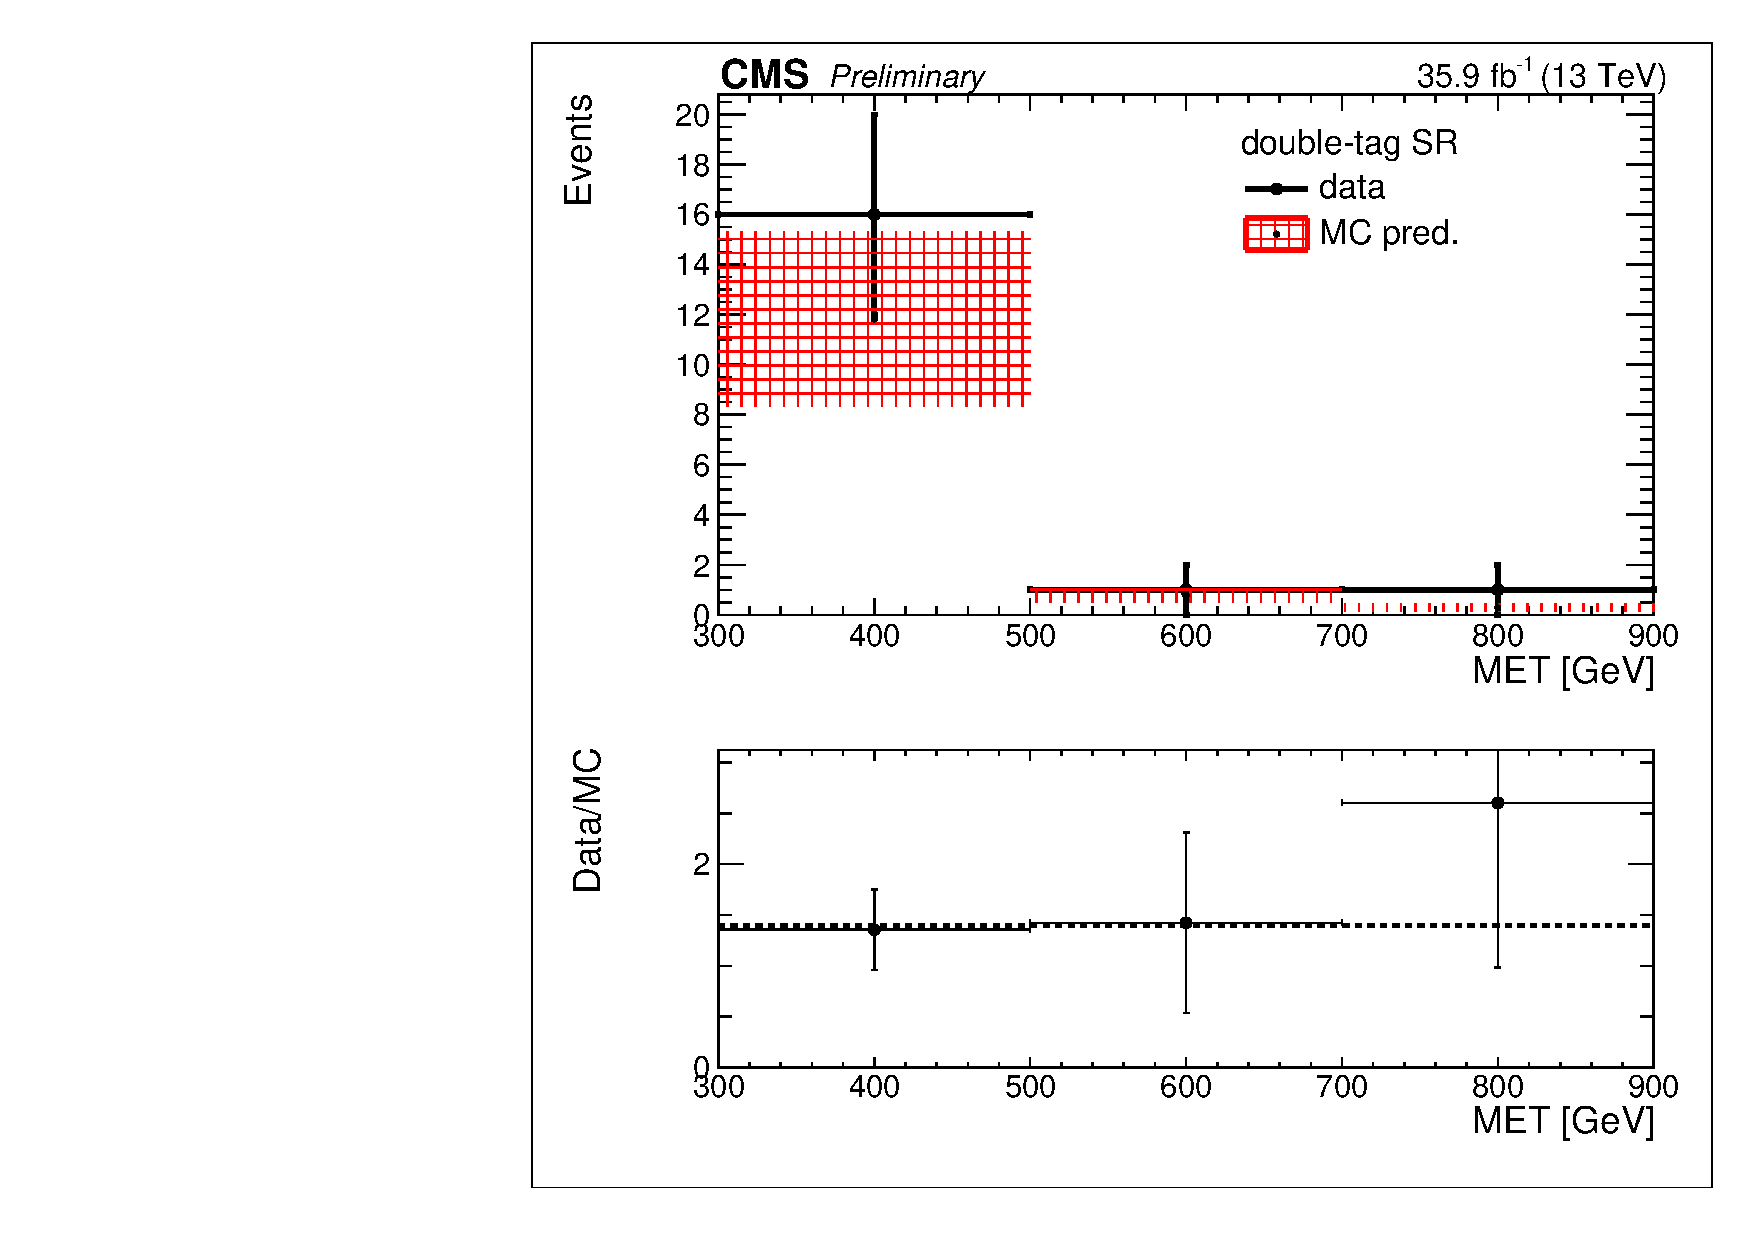
\includegraphics[trim={5px 5px 5px 5px},clip,width=0.425\linewidth]{figs/ABCDscaleFactors_MET_double-tagSR_lowDphi.pdf}\\
 \caption
 [Signal and sideband yields in the the low-$\Delta\phi$ control region.]
 {Signal and sideband yields in the the low-$\Delta\phi$ control region.The hashed red band denotes the prediction from simulation; the solid black points denote the observed yields in data. The Data/ ratio in the lower panel of each plot represents the scale factor for that bin. }
\label{fig:closurelowdphi}
\end{figure}

\begin{table}
\centering
\caption{Summary of the control region scale-factors integrated over \ptmiss.}
\label{tab:ScaleFactorVR}
\begin{tabular}{c|c|c|c|c|c}
\hline \hline
\multicolumn{6}{c}{Low $\Delta\phi$}\\
\hline \hline
$A^{1H}_{SF}$ & $A^{2H}_{SF}$ & $C_{SF}$ & $B^{1}_{SF}$ & $B^{2}_{SF}$ & $D_{SF}$  \\ \hline
   $1.1 \pm 0.33$ &$0.85 \pm 0.12$&  $0.93 \pm 0.1$ & $0.88 \pm 0.04$ & $1.2 \pm 0.16$  & $0.71 \pm 0.027$ \\ \hline
\hline \hline
\multicolumn{6}{c}{Single Lepton}\\
\hline \hline
$A^{1H}_{SF}$ & $A^{2H}_{SF}$ & $C_{SF}$ & $B^{1}_{SF}$ & $B^{2}_{SF}$ & $D_{SF}$  \\ \hline
   %$0.63 \pm 0.069$ & $0.64 \pm 0.15$  & \MET dependent &   $0.65 \pm 0.1$ & $0.71 \pm 0.059$  & \MET dependent\\ \hline
   %$0.64 \pm 0.033$ & $0.68 \pm 0.068$  & \MET dependent &   $0.63 \pm 0.011$ & $0.72 \pm 0.023$  & \MET dependent\\ \hline
   $0.61\pm 0.04$ & $0.59\pm0.08$ & \ptmiss dependent &  $0.59\pm 0.016$ & $0.71\pm 0.04$  & \ptmiss dependent\\ \hline
\hline \hline
\multicolumn{6}{c}{Photon}\\
\hline \hline
$A^{1H}_{SF}$ & $A^{2H}_{SF}$ & $C_{SF}$ & $B^{1}_{SF}$ & $B^{2}_{SF}$ & $D_{SF}$ \\ \hline
   $0.61 \pm 0.088$ & $0.75 \pm 0.29$ & $0.5 \pm 0.07$ & $0.98 \pm 0.094$ & $2.58 \pm 0.63$ & $0.71 \pm 0.035$\\ \hline
\end{tabular}
\end{table}

\begin{table}
\caption{Single lepton control region scale-factors in the anti-tag sideband region.}
\label{tab:ScaleFactorMET}
\centering
\begin{tabular}{|c|c|c|}
\hline\hline
\multicolumn{3}{c}{Single Lepton $C_{SF}$}\\
\hline
\ptmiss [300, 500] & [500, 700] & [700, $\infty$]\\
$0.47\pm0.05$ & $0.54\pm0.15$ & $0.18\pm 0.1$ \\  \hline\hline
\multicolumn{3}{c}{Single Lepton $D_{SF}$}\\
\hline
$0.49\pm0.02$ & $0.40\pm0.05$ & $0.35\pm 0.08$ \\  
\hline \hline
\end{tabular}
\end{table}

The scale factors are then applied to the  samples to give yields which better reflect data. The \ptmiss distributions for the signal regions and expectations from the ABCD background prediction are seen in Figure~\ref{fig:MCclosuresf} (the data-corrected version of Figure~\ref{fig:MCclosure}). The improved value of $\kappa$ is seen in the lower panel of each plot. The modified values of the  yields in the signal region (seen in the calculation of $\kappa$) are seen in Tables~\ref{tab:CorrSignal} ~and~\ref{tab:CorrControl}. Since most of the scale factors are less than one the background decreases in Figure~\ref{fig:MCclosure} relative to Figure~\ref{fig:MCclosuresf} but still preserves the normalization so that $\kappa$ is statistically compatible with unity. A distribution of $\kappa$ is derived by throwing gaussian toys for each of the scale factors, the final results being summarized in Table~\ref{tab:TotalKappa}.

\begin{table}
\caption{The $\kappa$ factor computed by throwing Gaussian toys for the scale factors.}
\label{tab:TotalKappa}
\centering
\begin{tabular}{c|c|c}
\hline \hline
& 1-Higgs Tag & 2-Higgs Tag\\
\hline \hline
\ptmiss &\multicolumn{2}{c}{$\kappa$} \\  \hline
% $\MET[300,500]$ & $1.03 \pm 0.15$ & $0.82 \pm 0.19$ \\ \hline
% $\MET[500,700]$ & $1.03 \pm 0.22$ & $0.53 \pm 0.17$ \\ \hline
% $\MET>700$ &  $0.83 \pm 0.18$ & $0.61 \pm 0.30$ \\ \hline
[300, 500 GeV] & $0.98 \pm 0.11$ & $0.73 \pm 0.14$ \\ \hline
[500, 700 GeV] & $0.86 \pm 0.16$ & $0.43 \pm 0.12$ \\ \hline
[700, $\infty$ GeV] &  $0.86 \pm 0.17$ & $0.62 \pm 0.30$ \\ \hline
\hline
\end{tabular}
\end{table}

\begin{figure}
\centering
\begin{subfigure}[b]{0.425\textwidth}
\centering
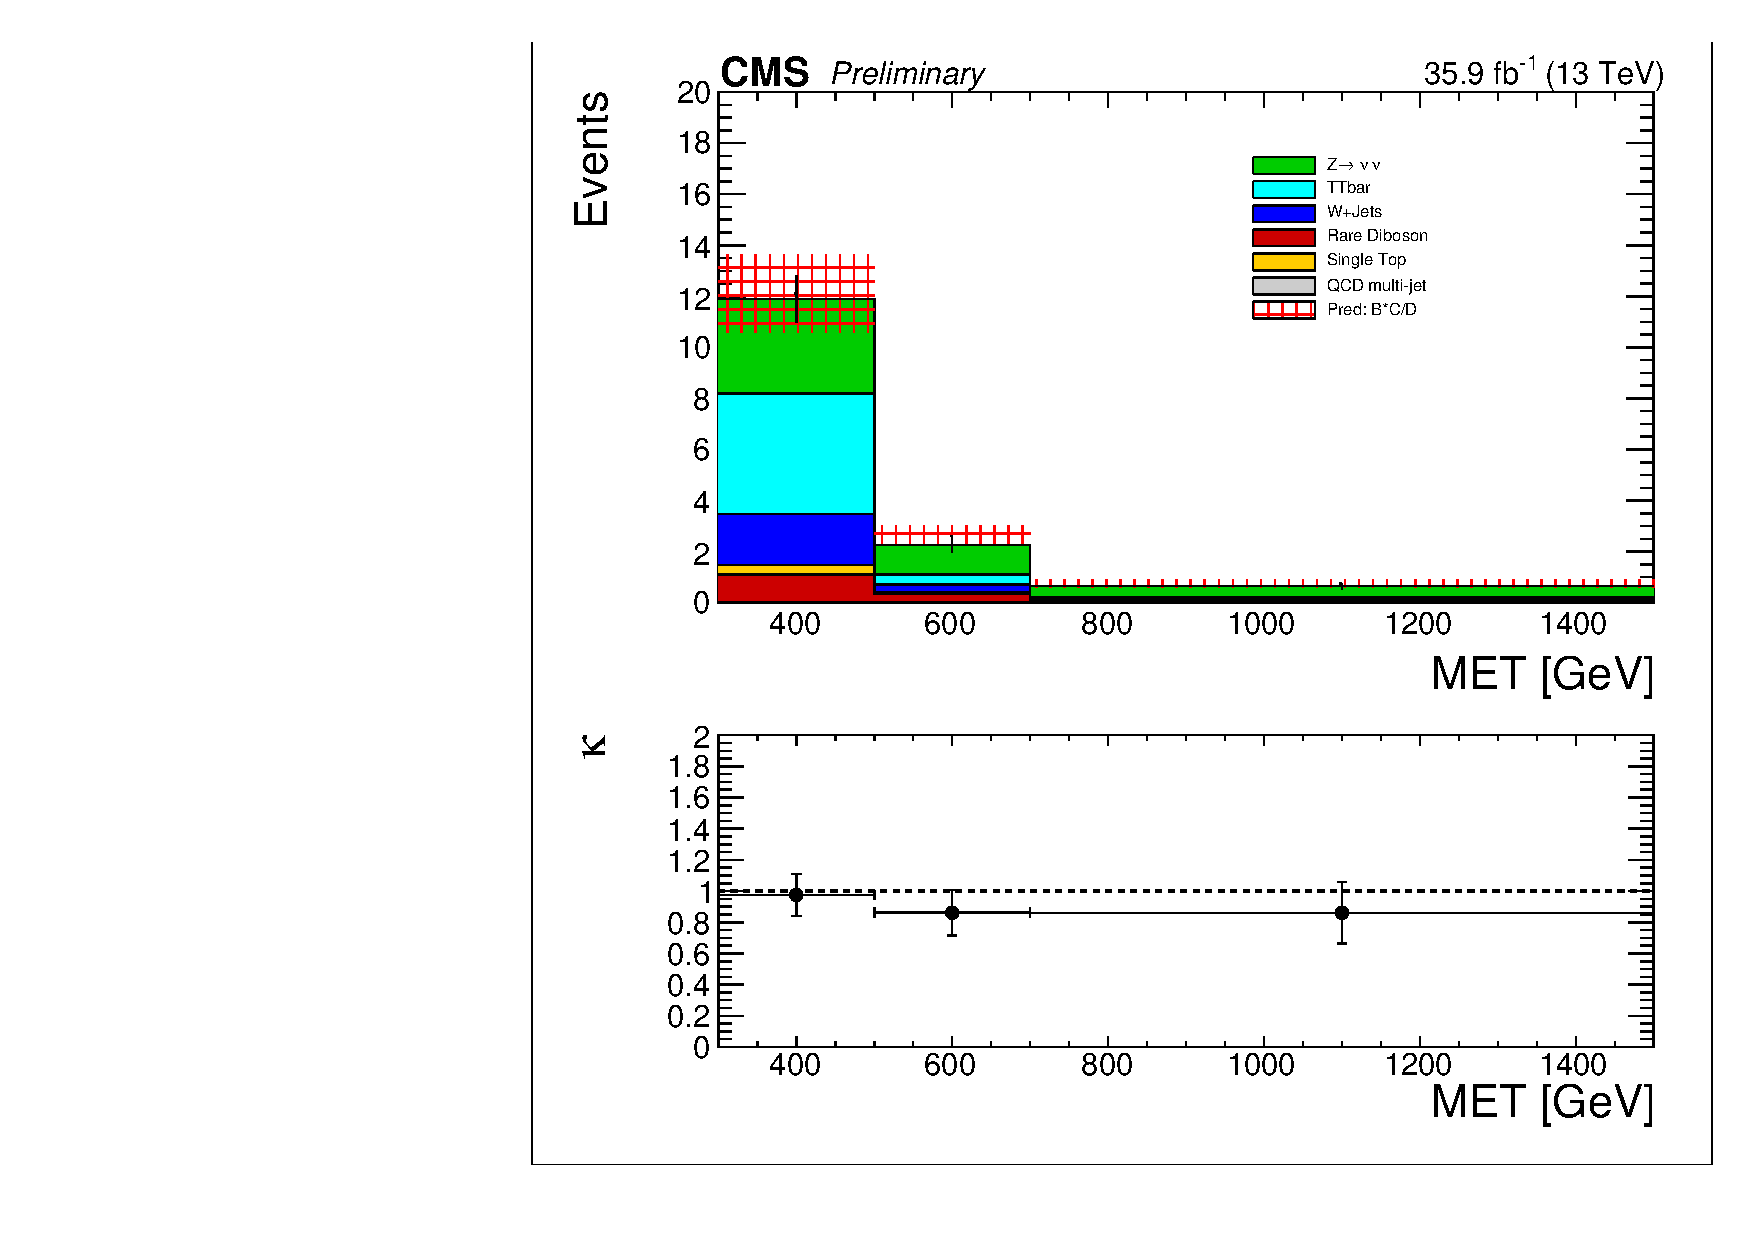
\includegraphics[trim={5px 5px 5px 5px},clip,width=0.95\textwidth]{figs/MCclosureSF_singleHiggsRegionTotal.pdf}
\caption{The single Higgs tag region (A$_{1}$).}
\end{subfigure}
\begin{subfigure}[b]{0.425\textwidth}
\centering
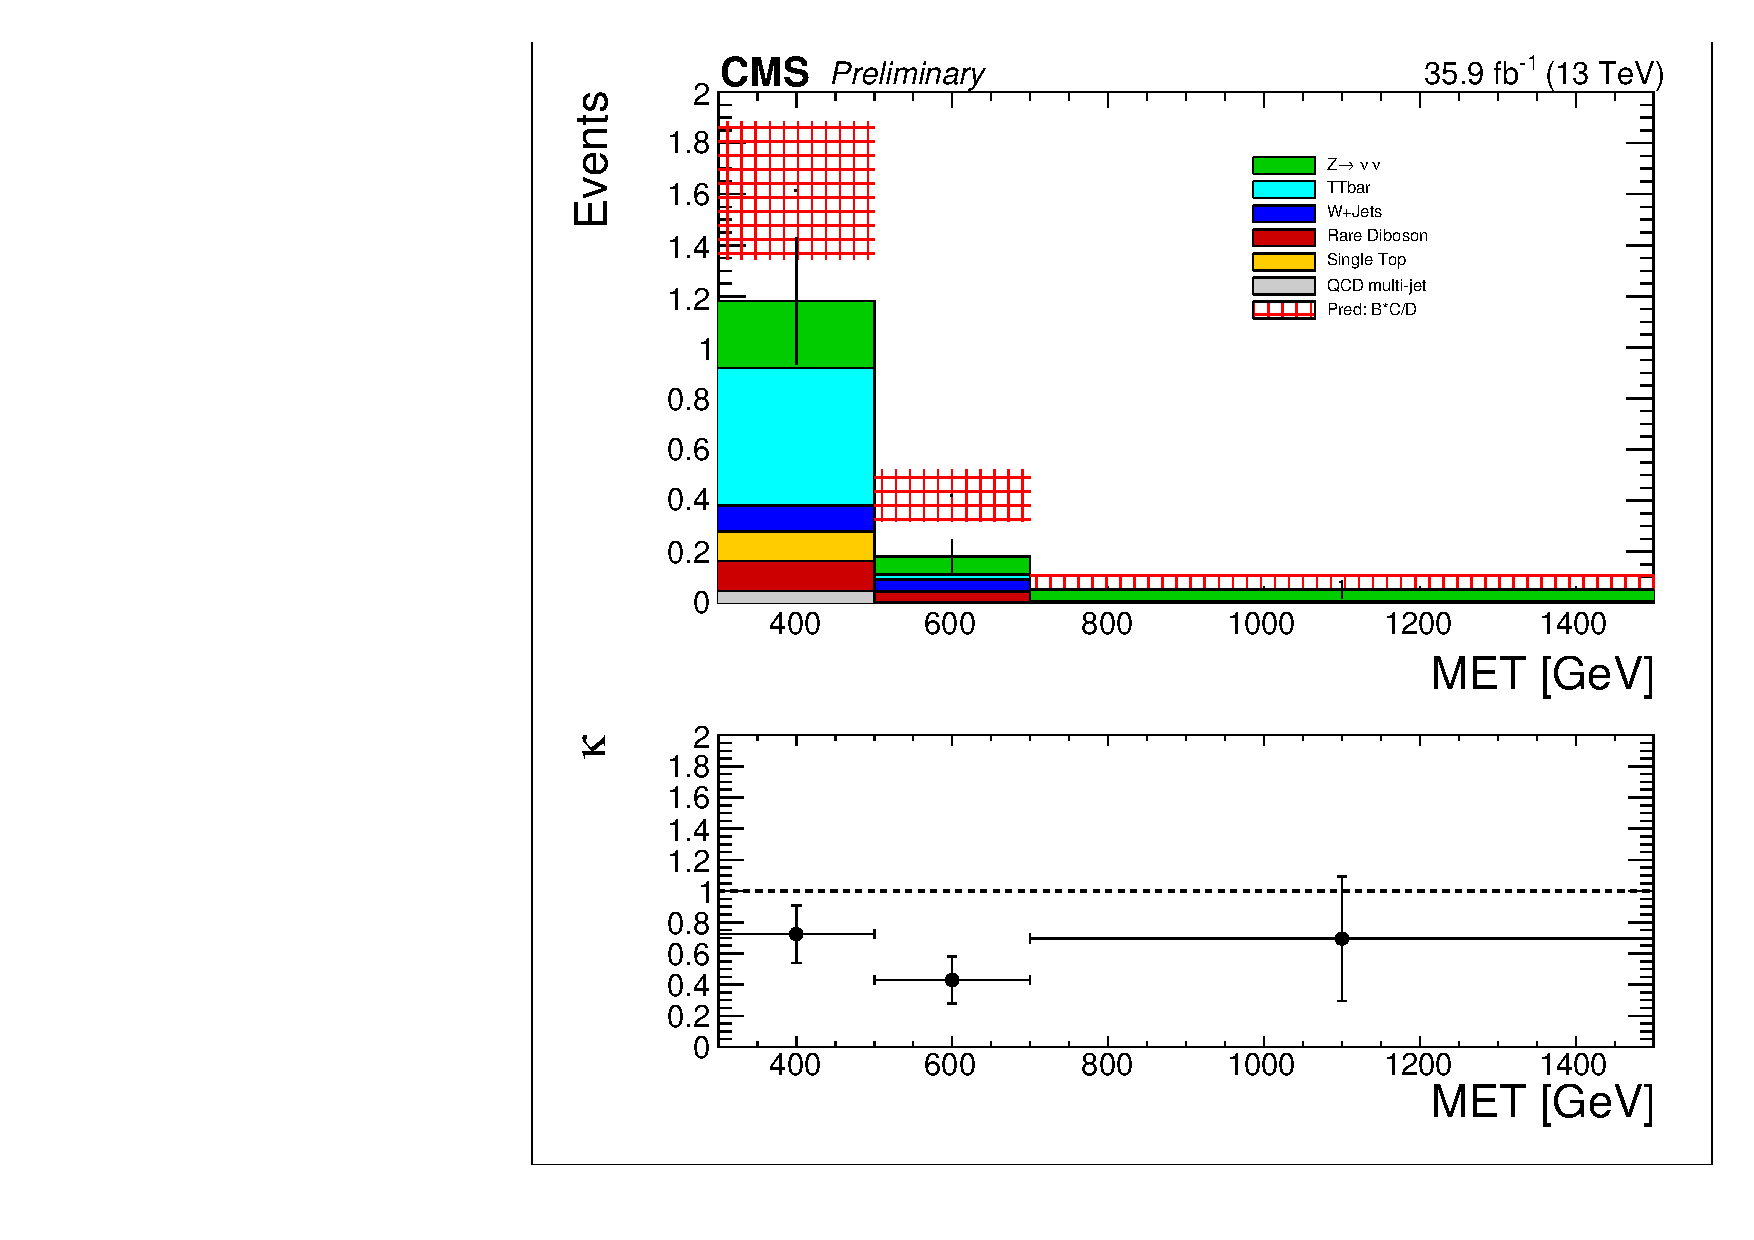
\includegraphics[trim={5px 5px 5px 5px},clip,width=0.95\textwidth]{figs/MCclosureSF_doubleHiggsRegionTotal.pdf} 
\caption{The double Higgs tag region (A$_{2}$).}
\end{subfigure}
\caption{Signal region \ptmiss distributions using scale-factor corrected simulation.}
\label{fig:MCclosuresf}
\end{figure}

\begin{landscape}
\begin{table}
\centering
\caption{Corrected  yields in the signal regions. $\kappa$ = AD / BC}
\begin{tabular}{c|c|c|c|c|c|c|c|}
\hline \hline
\ptmiss &  Z+Jets  & W+Jets & TTbar & QCD & Rare & Total  & Data \\ \hline \hline
\multicolumn{8}{c}{Region: $A^{1H}$}  \\ \hline \hline
$[300,500]$ GeV & 3.76 $\pm$ 0.54 & 2.05 $\pm$ 0.30 & 4.87 $\pm$ 0.72& 0 $\pm$ 0 & 1.48 $\pm$ 0.40 & 12.17 $\pm$ 1.03 &   15\\ \hline
$[500,700]$ GeV & 1.18 $\pm$ 0.21 & 0.33 $\pm$ 0.08 & 0.40$\pm$ 0.12& 0 $\pm$ 0 & 0.39$\pm$ 0.16 &   2.30 $\pm$ 0.29 & 2
\\ \hline 
$>700$ GeV & 0.43 $\pm$ 0.10 & 0.053$\pm$ 0.025& 0.046 $\pm$ 0.01& 0 $\pm$ 0 & 0.13 $\pm$ 0.053&   0.66$\pm$ 0.12& 1
\\ \hline
\multicolumn{8}{c}{Region: $A^{2H}$}  \\ \hline \hline
$[300,500]$ GeV & 0.26 $\pm$ 0.12 & 0.11 $\pm$ 0.05 & 0.58$\pm$ 0.21& 0.045$\pm$ 0.05 & 0.23$\pm$ 0.12   & 1.24 $\pm$ 0.28 & 1  \\ \hline
$[500,700]$ GeV & 0.07 $\pm$ 0.045 & 0.049 $\pm$ 0.031 & 0.022 $\pm$ 0.0098 & 0 $\pm$ 0 & 0.045 $\pm$ 0.039 &   0.19 $\pm$ 0.068 & 0\\  \hline
$>700$ GeV  & 0.044 $\pm$ 0.032& 0.005$\pm$ 0.005 & 0 $\pm$ 0 & 0 $\pm$ 0 & 0.002 $\pm$ 0.016  & 0.051 $\pm$ 0.036 &  0\\  \hline 
\end{tabular}
\end{table}
\begin{table}
\centering
\caption{Corrected  yields in the sideband regions. $\kappa$ = AD / BC} 
\label{tab:CorrSignal}

\begin{tabular}{c|c|c|c|c|c|c|c|}
\hline \hline
\ptmiss &  Z+Jets  & W+Jets & TTbar & QCD & Rare & Total  & Data \\
\hline \hline
\multicolumn{8}{c}{Region: $C$}  \\ \hline \hline
$[300,500]$ GeV & 17.66 $\pm$ 2.52 & 8.23 $\pm$ 1.44 & 3.87 $\pm$ 0.73 & 0.81 $\pm$ 0.49& 2.78 $\pm$ 1.142   & 33.36 $\pm$ 3.24 & 44 \\ \hline
$[500,700]$ GeV & 5.20$\pm$ 0.77& 0.57 $\pm$ 0.27 & 0.22 $\pm$ 0.11 & 0 $\pm$ 0 & 0.63 $\pm$ 0.16   & 6.63 $\pm$ 0.84 & 12
\\ \hline 
$>700$ GeV & 2.48 $\pm$ 0.39& 0.12 $\pm$ 0.12 & 0.028$\pm$ 0.031 & 0 $\pm$ 0 & 0.14 $\pm$ 0.06   & 2.76 $\pm$ 0.41 & 4
\\ \hline
\multicolumn{8}{c}{Region: $B^{1H}$}  \\ \hline \hline
$[300,500]$ GeV & 42.13 $\pm$ 4.17& 15.61 $\pm$ 10.15 & 30.99 $\pm$ 20.15 & 1.57 $\pm$ 0.54 & 12.16 $\pm$ 1.37   & 102.47 $\pm$ 23.00 & 112  \\ \hline
$[500,700]$ GeV & 12.05 $\pm$ 1.28 & 2.74 $\pm$ 1.79 & 3.04 $\pm$ 2.00 & 0 $\pm$ 0 & 2.55 $\pm$ 0.43   & 20.37 $\pm$ 3.00 & 20\\  \hline
$>700$ GeV  &5.92 $\pm$ 0.69& 0.67 $\pm$ 0.61& 0.49$\pm$ 0.46 & 0 $\pm$ 0 & 1.93 $\pm$ 0.72   & 9.01 $\pm$ 1.25 & 5  \\  \hline  
\multicolumn{8}{c}{Region: $B^{2H}$}  \\ \hline \hline
$[300,500]$ GeV & 5.51 $\pm$ 1.47 & 0.73 $\pm$ 0.44 & 4.46 $\pm$ 2.65 & 0.33 $\pm$ 0.23 & 2.06 $\pm$ 0.32 & 13.09 $\pm$ 3.09 & 13 
\\ \hline
$[500,700]$ GeV & 1.80 $\pm$ 0.56 & 0.17 $\pm$ 0.11 & 0.59 $\pm$ 0.39 & 0 $\pm$ 0 & 0.62 $\pm$ 0.23 & 3.17 $\pm$ 0.73 & 1 \\ \hline
$>700$ GeV  & 0.67 $\pm$ 0.27 & 0.0084 $\pm$ 0.009& 0.035 $\pm$ 0.031& 0 $\pm$ 0 & 0.23 $\pm$ 0.073   & 0.94 $\pm$ 0.28 & 1  \\  \hline  
\multicolumn{8}{c}{Region: $D$}  \\ \hline \hline
$[300,500]$ GeV & 164.82$\pm$ 8.31 & 61.24 $\pm$ 3.70 & 33.20 $\pm$ 2.16 & 8.50 $\pm$ 2.73 & 20.64 $\pm$ 1.78   & 288.41 $\pm$ 9.90 & 273  \\ \hline
$[500,700]$ GeV & 47.37 $\pm$ 2.52 & 6.36 $\pm$ 1.39 & 2.37 $\pm$ 0.55 & 0 $\pm$ 0 & 4.42$\pm$ 1.46 &   60.51 $\pm$ 3.27 & 60\\  \hline
$>700$ GeV  & 26.79 $\pm$ 1.50 & 0.99 $\pm$ 0.53 & 0.16 $\pm$ 0.086 & 0 $\pm$ 0 & 3.48 $\pm$ 1.01  & 31.42 $\pm$ 1.88& 28  \\  \hline  
\end{tabular}
\label{tab:CorrControl}
\end{table}
\end{landscape}

\subsection{Sideband Yields \& Predictions}

We have studied the background estimation technique in data and found the results to be acceptable. We then calculated $\kappa$, the correction to the ABCD prediction, using scale factors from data to best correct the normalization of the MC components. We can now use the observed yields in the sideband regions to form the background prediction via the ABCD method. Figure~\ref{fig:UnblindCR} shows the sideband yields in both data and the scale factor corrected MC - we see that the two agree within statistical errors. Table~\ref{tab:tab} tabulates the data yields alongside the full background prediction including $\kappa$.

\begin{figure}
\centering
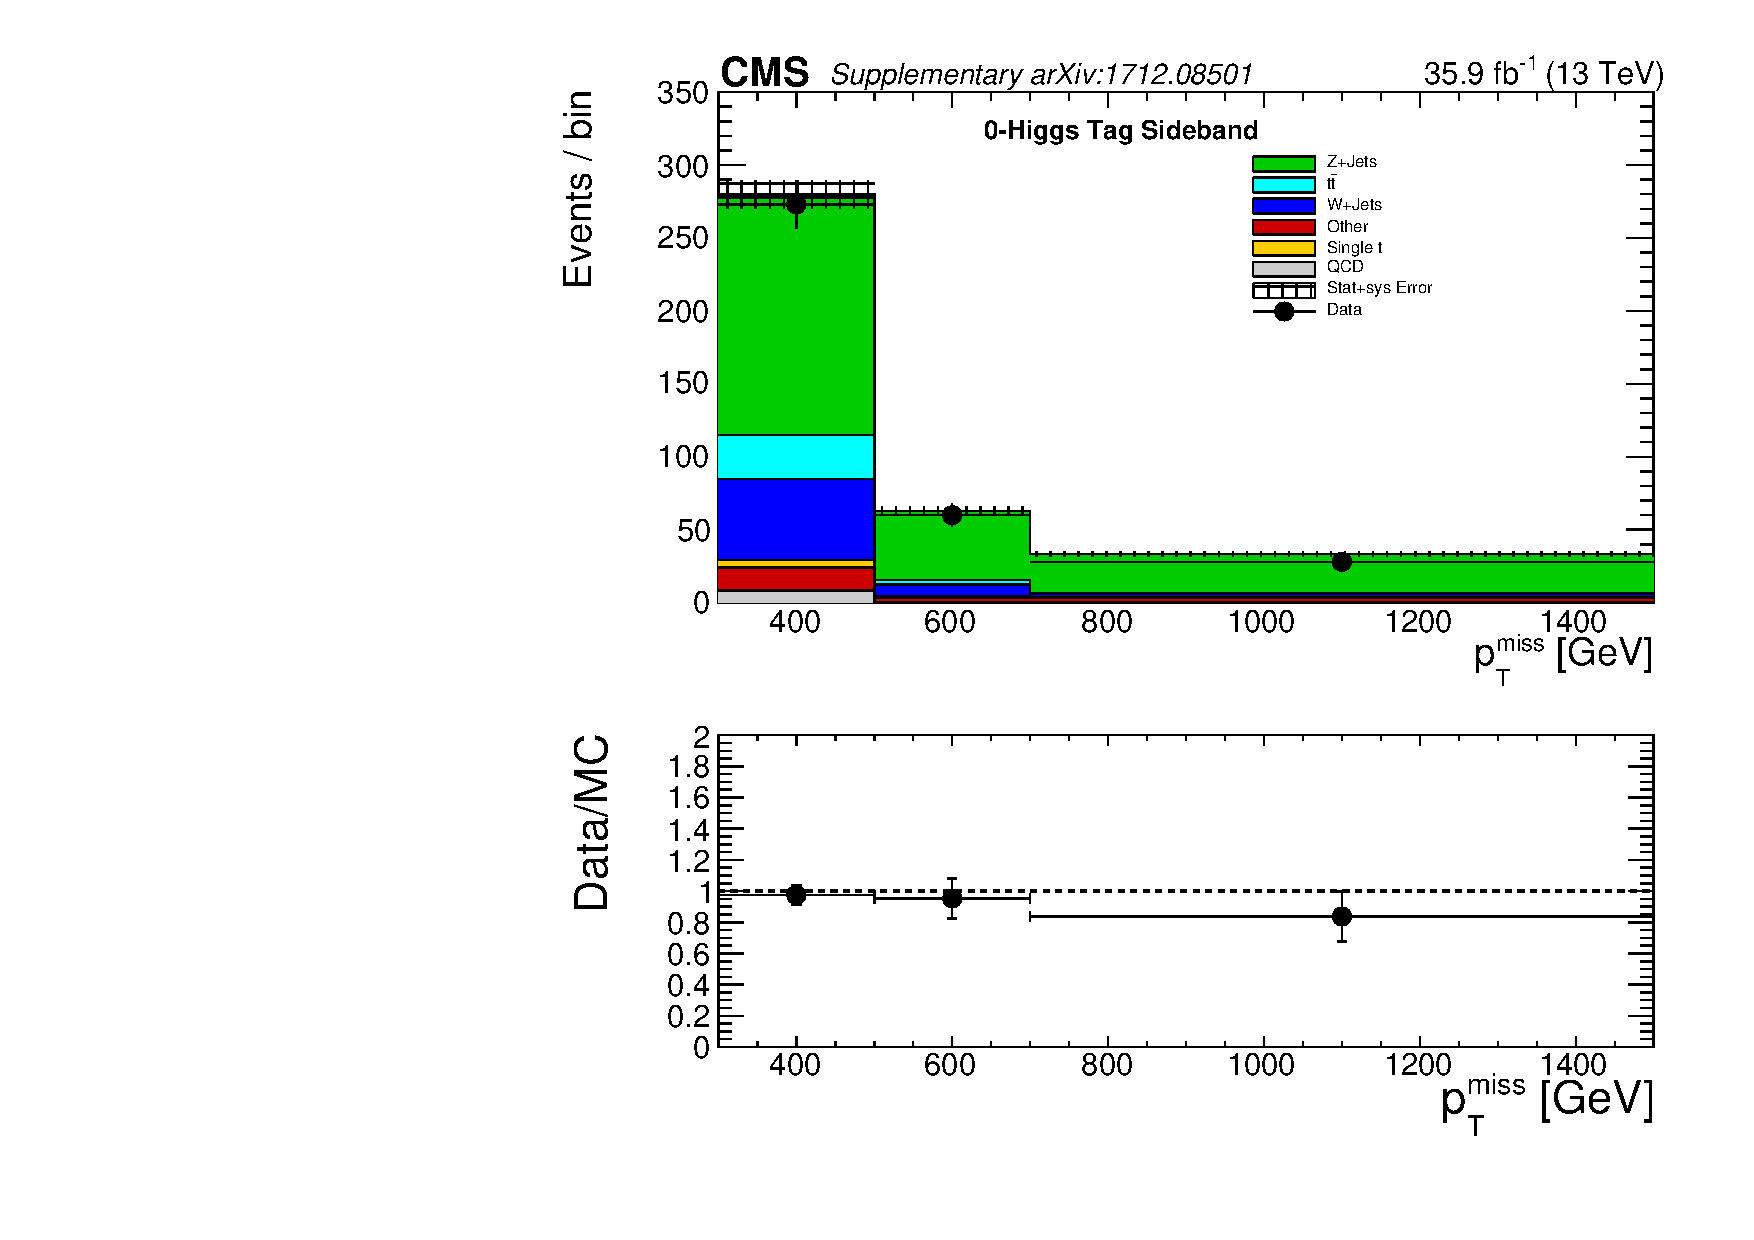
\includegraphics[trim={5px 5px 5px 5px},clip,width=0.425\linewidth]{figs/Unblinding_antitagSB.pdf}
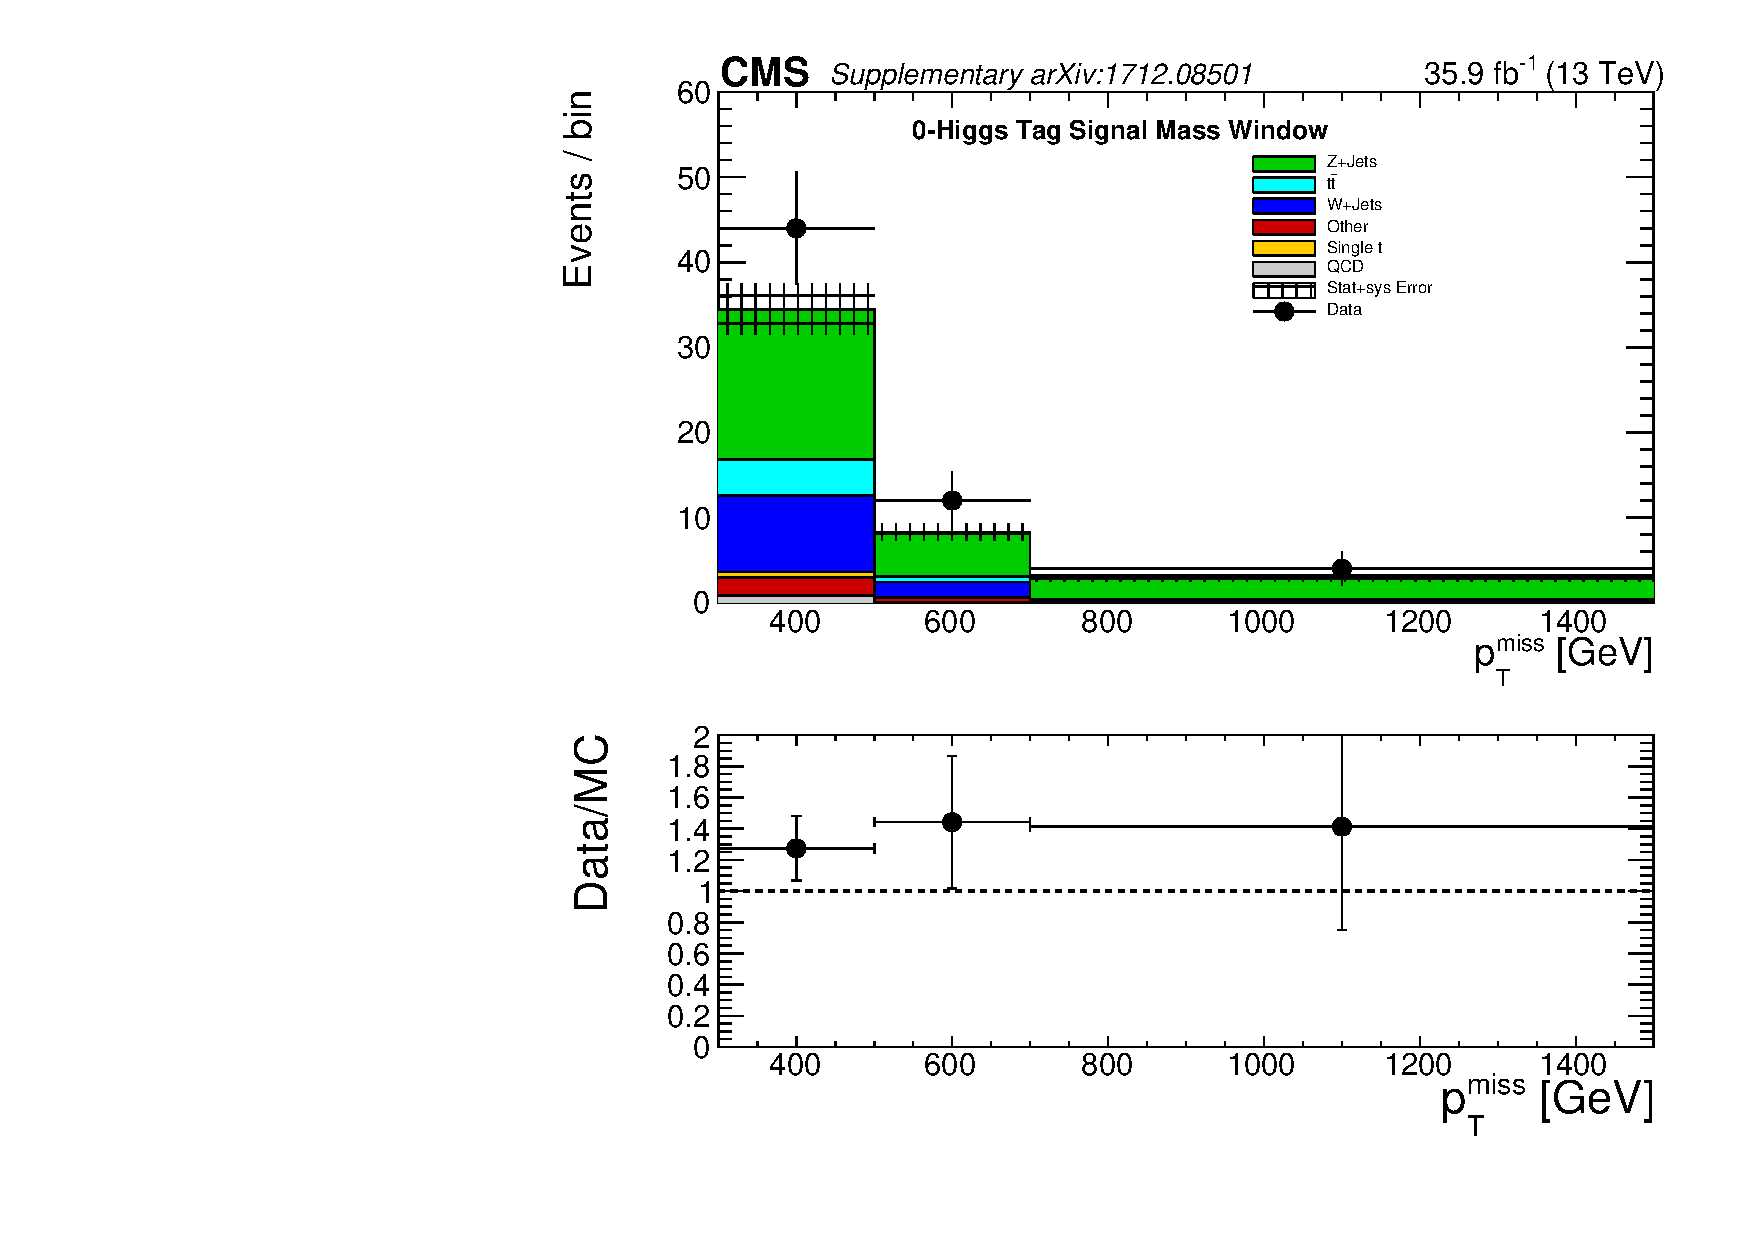
\includegraphics[trim={5px 5px 5px 5px},clip,width=0.425\linewidth]{figs/Unblinding_antitagSR.pdf}\\
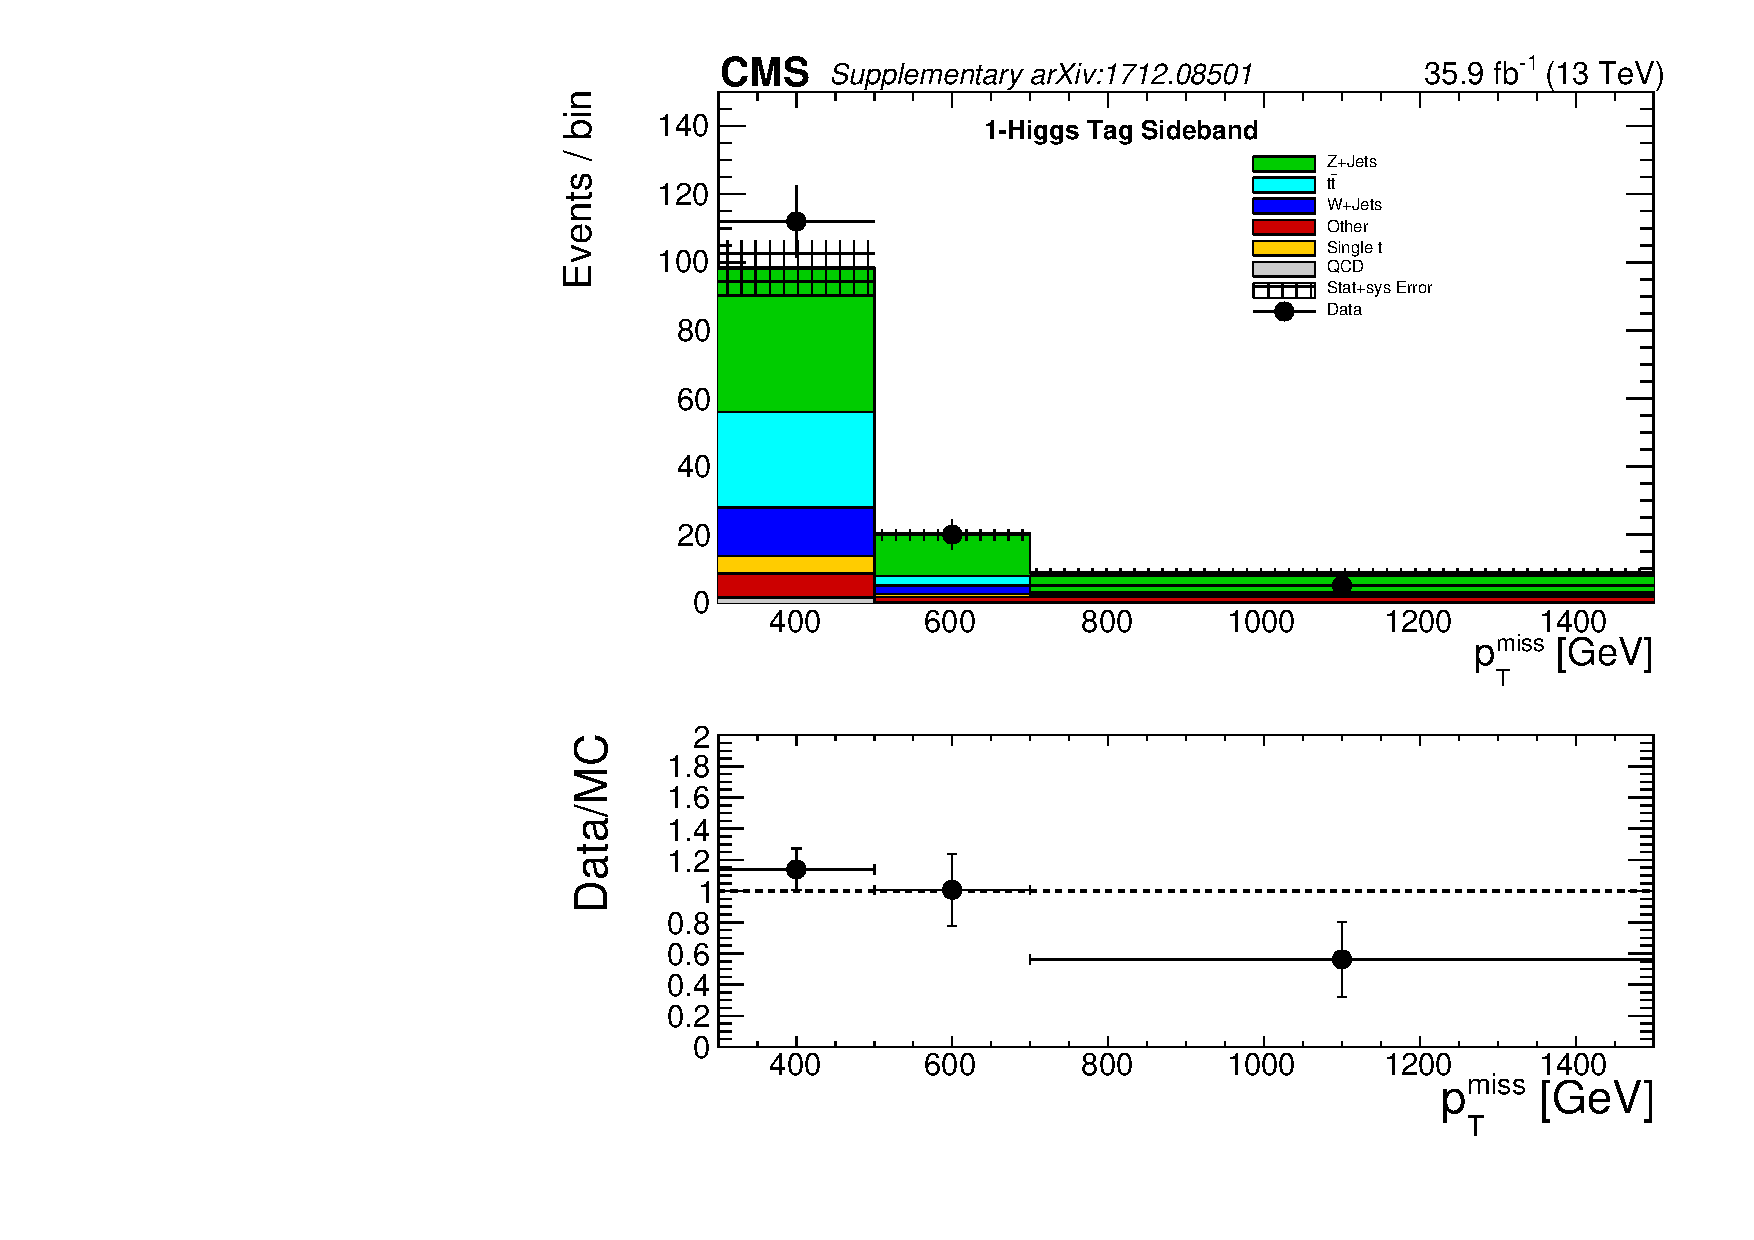
\includegraphics[trim={5px 5px 5px 5px},clip,width=0.425\linewidth]{figs/Unblinding_tagSB.pdf}
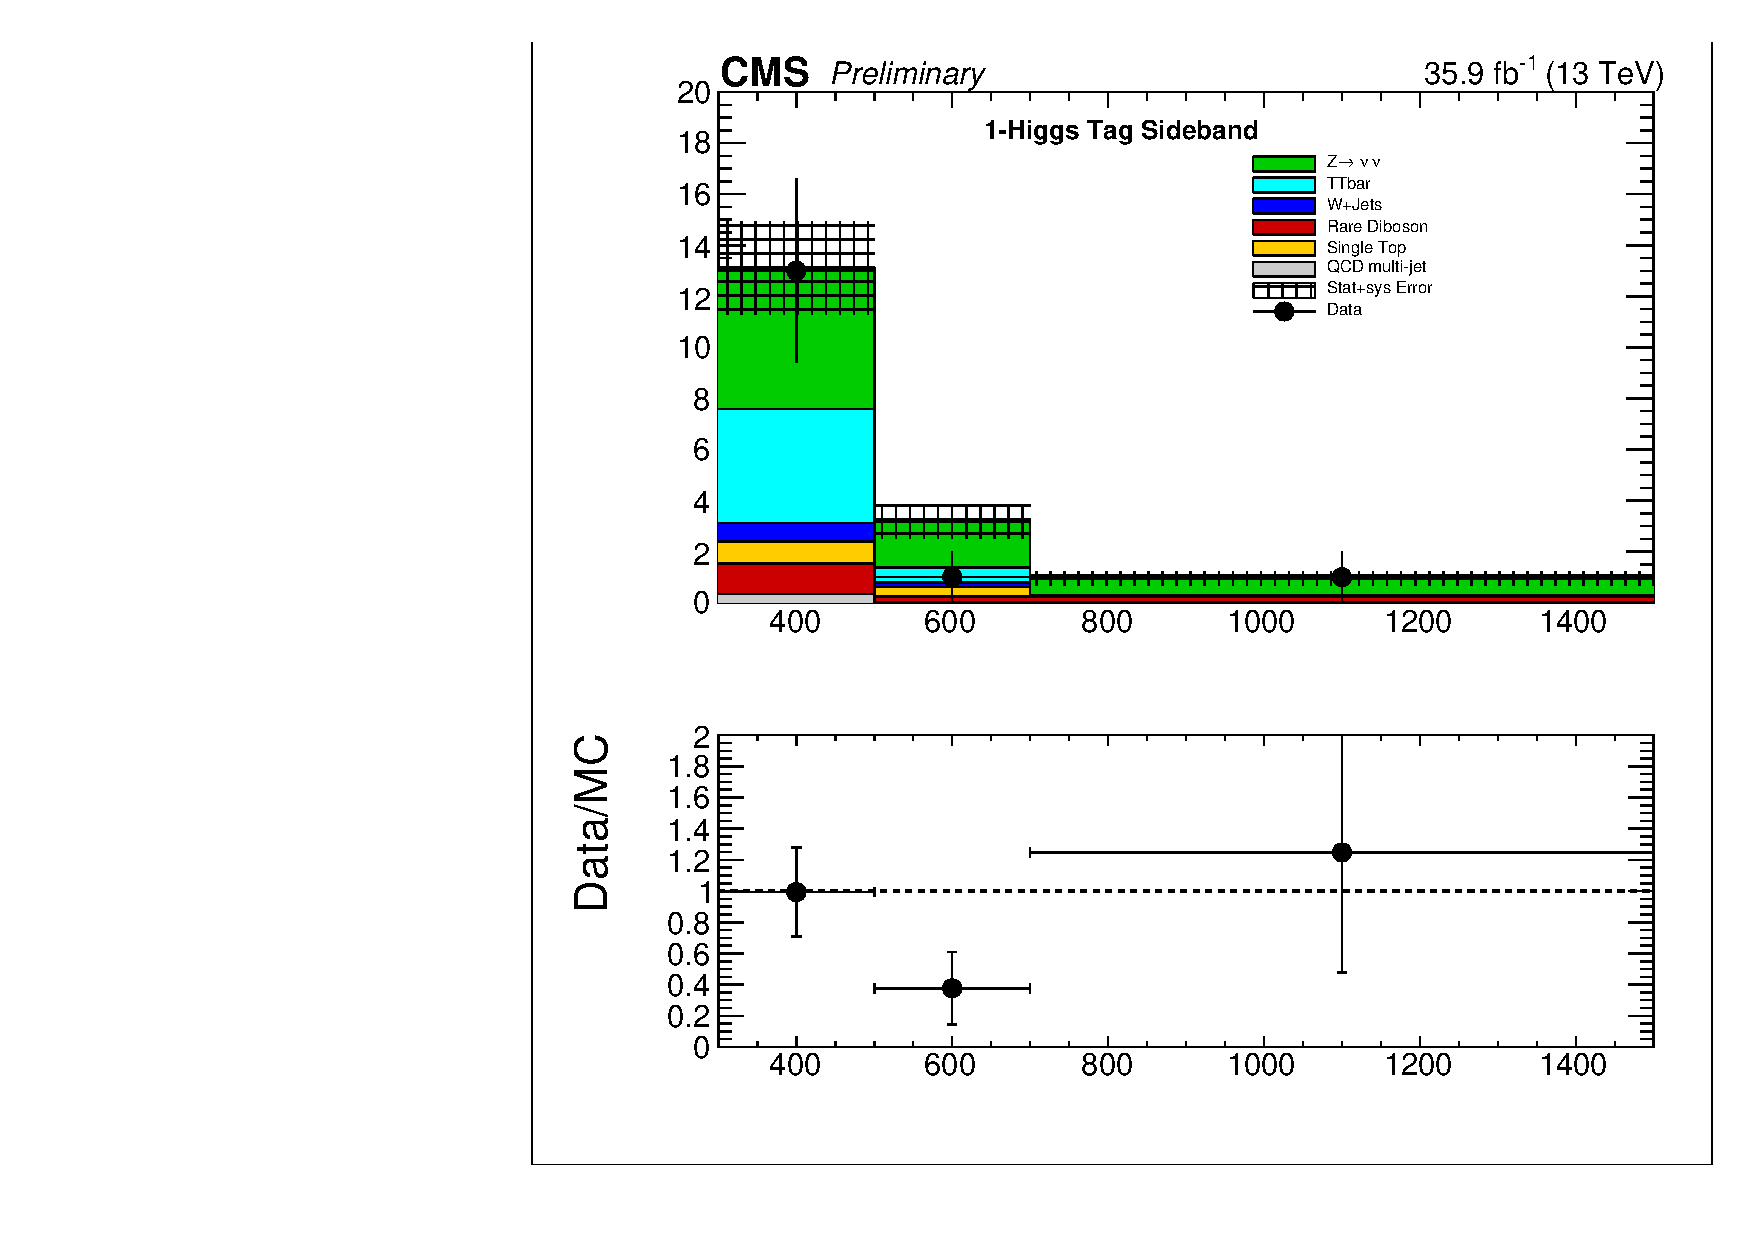
\includegraphics[trim={5px 5px 5px 5px},clip,width=0.425\linewidth]{figs/Unblinding_doubletagSB.pdf}\\
\caption
[Sideband region \ptmiss distributions of data and scale-factor corrected simulation.]{Sideband region \ptmiss distributions comparing data and scale-factor corrected simulation. The hashed red distribution denote the prediction from simulation; the solid points denote the observed yields in data.}
\label{fig:UnblindCR}
\end{figure}

\begin{table}
\centering
\caption{
Sideband region yields, $\kappa$, and background predictions for the 6 signal bins.
}
\begin{tabular}{lllllll}
\hline
\hline
$N_{\mathrm{H}}$ & $p_{T}^{\mathrm{miss}}$ (GeV) & B & C & D & $\kappa$  & $\kappa \cdot B \cdot C / D$ \\
\hline
$A_{1}$ & [300, 500 GeV]      & 112 & 44  & 273 & 0.98 $\pm$ 0.11 & 17.7 $\pm$ 3.8\\
$A_{1}$ & [500, 700 GeV]      & 20   & 12  & 60   & 0.86 $\pm$ 0.16 & 3.4  $\pm$ 1.5\\
$A_{1}$ & [700, $\infty$ GeV] & 5    & 4    & 28   & 0.86 $\pm$ 0.17 & 0.61 $\pm$ 0.45\\
$A_{2}$ & [300, 500 GeV]      & 13   & 44  & 273 & 0.73 $\pm$ 0.14 & 1.52 $\pm$ 0.57\\
$A_{2}$ & [500, 700 GeV]      & 1     & 12  & 60   & 0.43 $\pm$ 0.12 & 0.09 $\pm$ 0.08\\
$A_{2}$ & [700, $\infty$ GeV] & 1     & 4     & 28   & 0.62 $\pm$ 0.30 & 0.09$^{+0.11}_{-0.09}$\\
\hline
\hline
\end{tabular}
\label{tab:tab}
\end{table}

\section{Signal Systematics}
\label{sec:signalsys}
We consider a variety of systematic uncertainties on the signal efficiency and distribution. Some are common to more 
inclusive SUSY analyses \cite{RA2b:Moriond} and there are additional systematics related to $b\bar{b}$ tagging efficiency and 
the effect of the pruned mass scale and resolution on the signal efficiency.  
\begin{itemize}
\item {\bf Luminosity:} The recommendation for the 2016 dataset is currently a flat uncertainty of 2.5\%.
\item {\bf Isolated track veto:} A flat uncertainty of 2\% is assigned to the signal samples to account for any data/ differences based on the study from the 2015 analysis \cite{RA2b:Moriond}.
\item {\bf  statistics:} The sign fal  sample statistical uncertainty is generally 2-4\% .
\item {\bf Trigger efficiency:} The effect of the uncertainty on the signal yield is about 2\%.
\item {\bf Pileup reweighting:} The sensitivity to the pileup distribution was studied for various benchmark signal models by comparing events with $n_{\textrm{vtx}} < 20$ (low PU) or $n_{\textrm{vtx}} \geq 20$ (high PU). Accordingly, no pileup reweighting is applied to the signal  samples and no associated uncertainty is assessed.
\item {\bf ISR:} An ISR correction is derived from tt events, with a selection requiring two lep-
tons (electrons or muons) and two b-tagged jets, implying that any other jets in the
event arise from ISR. The correction factors are 1.000, 0.920, 0.821, 0.715, 0.662, 0.561,
0.511 for NISR = 0, 1, 2, 3, 4, 5, 6+. The corrections are applied to the simulated signal jet
samples with an additional normalization factor, typically ∼1.15 (depending on the signal model), to ensure the overall cross section of the sample remains constant. The systematic uncertainty in these corrections is chosen to be half of the deviation from unity for each correction factor. The effect on the yield ranges from $0.0–1\%$, with the largest effect at high \ptmiss.
\item {\bf Scales:} The uncertainty is calculated using the envelope of the weights from varying the renormalization and factorization scales, $\mu_{R}$ and $\mu_{F}$,by a factor of 2 \cite{Cacciari:2003fi, Catani:2003zt}. The effect on the yield of is less than 0.1\%.
\item {\bf Jet Energy Corrections:} The jet energy corrections (JECs) are varied using the $p_{T}$-
and $\eta$-dependent jet energy scale uncertainties from the official database.
These variations are propagated into the various jet-dependent variables, including: $H_{T}$, MET, $\Delta\phi(\textrm{MET},j_{i})$.
The overall effect is less than 1\%.
\item {\bf Jet Energy Resolution:} The jet momenta in the  samples are smeared to match the jet energy resolution in data. The smearing factors are varied according to the uncertainties on the jet energy resolution measurements.
These variations are propagated into the various jet-dependent variables, including: $H_{T}$, MET, $\Delta\phi(\textrm{MET},j_{i})$.
The overall effect ranges from 0.01\%.
\item {\bf PDFs:} The LHC4PDF prescription for the uncertainty on the total cross section is included as $\pm 1$ sigma bands in the results plots. No
additional uncertainty is considered for the uncertainty in the acceptance due to PDFs, as per SUSY group recommendation.
\end{itemize}
The above signal systematics are applied as an uncertainty on the signal normalization. These uncertainties are in general small. The main signal systematics 
come from the AK8 Jet Double-b tagging efficiency data/ scale factors and the uncertainty on the pruned mass resolution.
The AK8 Jet Double-b tagging efficiency has an uncertainty which is propagated to the signal efficiency. This uncertainty is applied 
as a shape uncertainty across the Higgs tag regions and the anti-tag region. Also the pruned jet mass scale and resolution uncertainties are 
propogated to the final signal efficiency using POG recommendations. The pruned mass scale factor is derived using W-jets in semi-leptonic \ttbar and extrapolating to the H mass. This uncertainty is assigned a shape uncertainty on the signal mass window and the sideband. \\
\begin{itemize}
\item A data/ scale-factor is derived from double-muon tag data selected with HLT Trigger \texttt{HLT\_BTagMu\_AK8Jet300\_Mu5\_v} and muon enriched QCD Monte-Carlo. The scale factors have mainly a statistical error along with a smaller set of systematic errors due to shape systematics, Jet-Energy scale uncertainty, Pile-up corrections, uncertainty on the number of tracks, uncertainty of b-fragmentation and  c-fragmentation, and the uncertainty on $K_{s}$ and $\Lambda$ fraction. 
\item The pruned mass scale-factor is derived by comparing the efficiency to select W-jets in data and  within a mass window of $\left[65,85\right]$ GeV.  The fit for the gaussian resolution of the W-mass peak is shown in Figure~\ref{fig:WMassPeak} and the fit results are shown in Table~\ref{tab:WMassFit}. The mass scale between  and data is consistent though  predicts a narrower mass resolution compared to data. The jet mass in each event is smeared to mimic the pruned jet mass resolution in data and an uncertainty is assigned based on the ratio of efficiencies between the smeared and un-smeared cases~\cite{CMS_AN_2016-215}.
\end{itemize} 

The summary of the signal systematics and their effect on the signal yields is shown in Table~\ref{tab:SignalSystSummary}. The dominant effect is from the mass resolution uncertainty.
%\item The pruned mass scale-factor is found to be consistent with 1.0 for the pruned mass-scale with an uncertainty based on the Jet-Energy scale uncertainty: $\sqrt{JES^2 + 0.02^2}$. The pruned jet mass-resolution scale-factor is found to $7\%$ with an uncertainty of $\sqrt{JER^2+0.103^2}$

\begin{figure}
\begin{center}
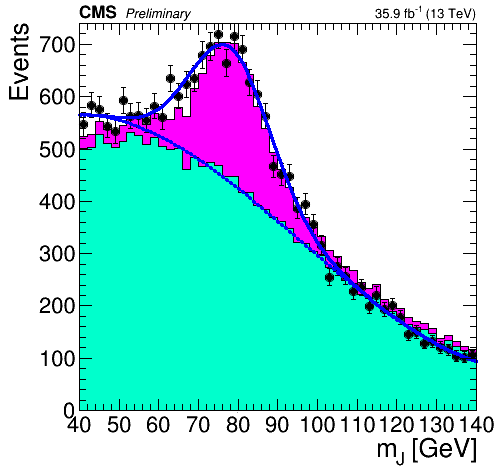
\includegraphics[width=0.5\linewidth]{figs/WMassPeakDataMC.png}
\end{center}
\caption
[Pruned jet mass in semi-leptonic \ttbar events.]
{Pruned jet mass in semi-leptonic \ttbar events. The mass peak for the W-jets is used to derive the mass resolution uncertainty.}
\label{fig:WMassPeak}
\end{figure}

\begin{table}
\caption{Fit results for W-mass resolution in data and simulation.}
\label{tab:WMassFit}
\centering
%\hline\hline
\begin{tabular}{c||c|c}
\hline
\hline
% & \multicolumn{1}{c}{Data} & \multicolumn{1}{c}{$t\bar{t}$}\\
 & Data & $t\bar{t}$\\
\hline
Mean & 78.2$\pm$0.46 & 78.4$\pm$0.35\\
Sigma & 10.10$\pm$0.67 & 7.23$\pm$0.48\\
\hline
\hline
\end{tabular}
\end{table}

\begin{table}
\centering
\begin{tabular}{c|c}
\hline \hline
\multicolumn{2}{c}{Unc. on Normalization} \\  \hline
\hline \hline
Systematic & \% Effect on yields\\ \hline
Luminosity & 2.6\% \\ \hline
Trigger Eff. & 2.0\% \\ \hline
Iso. Track Veto & 2\%\\ \hline
ISR modeling & 0.01\% \\ \hline
PDF Scale & 0.1\% \\ \hline
JEC & 1\% \\ \hline
JER & 0.01\% \\ \hline
 Stat & 1-4\% \\ \hline
\multicolumn{2}{c}{Shape Unc.} \\  \hline
Double-b SF & 6\% \\ \hline
Mass Resolution &1-15\% \\ \hline
\hline
\end{tabular}
\caption{
    Summary of signal shape and normalization uncertainties. 
}
\label{tab:SignalSystSummary}
\end{table}

\section{Observed Yields in the Signal Regions}
\label{sec:results}

The observed yields, along with the background predictions, are seen in Table~\ref{tab:DataPred}. Our signal region yields are consistent with the background expectation. Additionally, Table~\ref{tab:DataPred} shows the expected signal yields for two model points corresponding to gluino $\tilde{g}$ masses of 2000 or 1800 GeV; the mass of the neutralino $\tilde{\chi}_{1}^{0}$ is fixed at 1 GeV; the mass splitting between the gluino $\tilde{g}$ and neutralino $\tilde{\chi}_{2}^{0}$ is fixed at 50 GeV.

\begin{figure}
\centering
\begin{subfigure}[b]{0.425\textwidth}
\centering
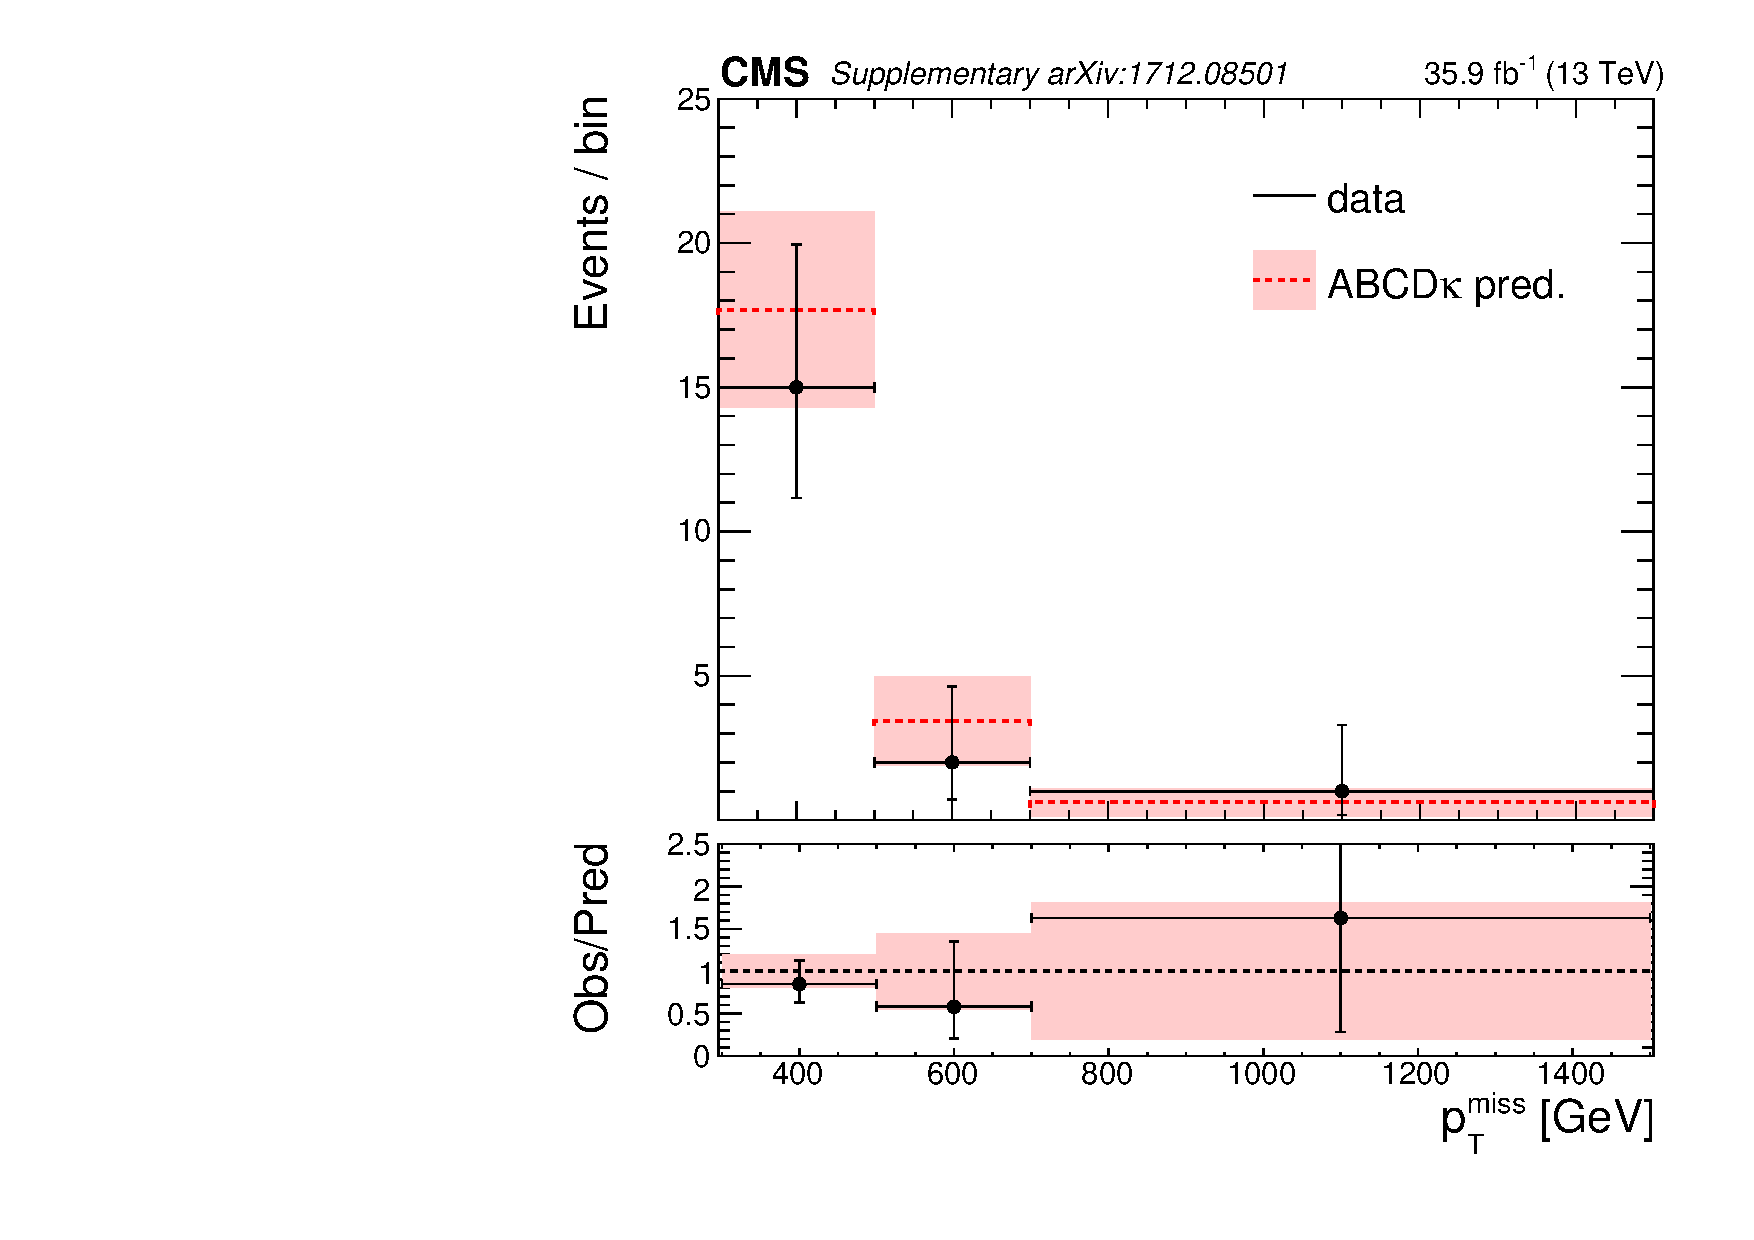
\includegraphics[trim={5px 5px 5px 5px},clip,width=0.95\textwidth]{figs/CMS-SUS-17-006_Figure-aux_004.pdf}
\caption{The single Higgs tag region (A$_{1}$).}
\end{subfigure}
\begin{subfigure}[b]{0.425\textwidth}
\centering
\includegraphics[trim={5px 5px 5px 5px},clip,width=0.95\textwidth]{figs/CMS-SUS-17-006_Figure-aux_005.pdf} 
\caption{The double Higgs tag region (A$_{2}$).}
\end{subfigure}
\caption{Observed yields in the signal regions.}
\label{fig:datayields}
\end{figure}

\begin{table}
\caption[Yields and predicted background in the signal regions.]{Yields and predicted background in the signal regions. Columns 2, 3, and 4 form the background prediction. Obs. represents the observed yields in data. The last two columns represent the expected yields from two model points (the gluino mass is in parenthesis).}
\label{tab:DataPred}
\centering
\begin{tabular}{l|c|c|c|c||c|c|}
\hline \hline
\ptmiss & $B \cdot C / D$ & $\kappa$ & $\kappa \cdot B \cdot C / D$ & Obs. & T5HH(2000) & T5HZ(1800) \\
\hline \hline
\multicolumn{7}{c}{1-Higgs Tag} \\ \hline \hline
[300, 500 GeV]      & $18.05 \pm 3.39$  & $0.98 \pm 0.11$ & $17.68 \pm 3.85$ & 15 & 0.24 & 0.75  \\ \hline
[500, 700 GeV]      & $4 \pm 1.54$ & $0.86 \pm 0.16$ & $3.44\pm 1.47$ &  2  & 0.32 & 0.98 \\\hline
[700, $\infty$ GeV] &  $0.71 \pm 0.50$  &  $0.86 \pm 0.17$ & $0.61\pm 0.45$ &  1 & 2.13 & 4.34\\\hline \hline
\multicolumn{7}{c}{2-Higgs Tag} \\  \hline \hline
[300, 500 GeV]       &   $2.09 \pm 0.67$  & $0.73 \pm 0.14$ & $1.52 \pm 0.57$ & 1 & 0.17 & 0.35\\ \hline
[500, 700 GeV]       & $ 0.2 \pm 0.20$ & $0.43 \pm 0.12$ &$0.09^{+0.08}_{-0.08}$ & 0 & 0.23 & 0.44\\ \hline
[700, $\infty$ GeV] & $0.14 \pm 0.16$ & $0.62 \pm 0.30$ & $0.09^{+0.11}_{-0.09}$ & 0 & 1.36 & 1.98\\ \hline
\hline
\end{tabular}
\end{table}

A visual representation of the one event in the double-H tagged signal bin is seen in Figure~\ref{fig:fireworks}. The purple line represents \ptmiss=426 GeV. The three yellow cones represent the AK8 jets labeled with $p_{T}$.  Note the two additional objects not satisfying our object definition but still plotted in the representation a) the additional low-$p_{T}$ and low mass AK8 jet b) the $p_{T}$=18 GeV muon (red line) suffers from poor reconstruction properties.

\begin{figure}
\centering
\begin{subfigure}[b]{0.4\textwidth}
\includegraphics[width=\textwidth]{figs/fireworks_ak8barrel.png}
\end{subfigure}
\begin{subfigure}[b]{0.4\textwidth}
\includegraphics[width=\textwidth]{figs/fireworks_ak8rhophi.png}
\end{subfigure}
\caption{The single event in the $A_{2}$ region.}
\label{fig:fireworks}
\end{figure}

\section{Exclusion Curves \& Mass Limits}

Interpreting our results in the context of the T5HH or T5ZH models, the absence of signal allows us to place lower limits on the cross section of gluino $\tilde{g}$ pair production. For the statistical treatment, we use a profile-likelihood to combine the observed yields, expected background, and expected signal in all analysis bins to calculate a 95\% upper limit on the signal cross section. The ABCD background estimation is explicitly coded in the likelihood, allowing the correlations in the estimations to be taken into account. The likelihood function can be expressed as:

\begin{equation}
\mathcal{L}=\prod_{i \in A, B, C, D}\mathrm{Poisson}\left(n_i \vert bkg_i + r\cdot sig_i\right) \times \prod^{nuisances}_j \mathrm{Constraints}\left(\theta_j , \hat{\theta}_j\right)
\end{equation}

where the regions are modeled by Poisson distributions, n$_{i}$, $bkg_{i}$, and $sig_{i}$ represent the yield, expected background, and  expected signal in bin i. The constraints term encode the nuisance parameters $\theta_{j}$: $\kappa$ is modeled by a normal distribution, and the signal systematics are modeled as log-normal. The term $\hat{\theta}_{j}$ represents the profiled minima of $\theta_{j}$. 

The expected and observed limits are then calculated based on approximations of the profile likelihood ratio using the CLs criterion to place upper limits at the $95\%$ confidence level on the production cross section, as seen in Figure~\ref{fig:brazil}. The allowed regions lie below the red and blue lines. Calculations of the gluino pair production cross section \cite{ggcs}, seen in the black line, allow us to rule out gluinos with mass lower than 2010 and 1825 GeV for the T5HH and T5ZH models, respectively. The weaker limit for the T5ZH model is due to the smaller branching fraction of the Z boson to b-quarks and our choice of signal mass window not being optimal for Z reconstruction.

\begin{figure}
\centering
\begin{subfigure}[b]{0.49\textwidth}
\includegraphics[width=\textwidth]{figs/brazilT5HHResults.pdf}
\caption{T5HH}
\end{subfigure}
\begin{subfigure}[b]{0.49\textwidth}
\includegraphics[width=\textwidth]{figs/brazilT5HZResults.pdf}
\caption{T5ZH}
\end{subfigure}
\caption{Observed and expected limits on the gluino cross section.}
\label{fig:brazil}
\end{figure}
